\documentclass[a4paper,11pt,twoside]{report}
% KOMPILOWAĆ ZA POMOCĄ pdfLaTeXa

% -------------- Kodowanie znaków, język polski -------------
\usepackage[utf8]{inputenc}
\usepackage[MeX]{polski}
\usepackage[T1]{fontenc}
\usepackage[english,polish]{babel}

% -------------- Pakiety matematyczne i techniczne -------------
\usepackage{amsmath,amsfonts,amssymb,amsthm,latexsym}
\usepackage[final]{pdfpages}
\usepackage{commath}
\usepackage{graphicx}
\usepackage{booktabs}
\usepackage{array}
\usepackage{longtable}
\usepackage{float}
\usepackage{caption}
\usepackage{subcaption}
\usepackage{enumitem}
\usepackage{csquotes}
\usepackage[hidelinks]{hyperref}
\usepackage{bbm}

% -------------- Bibliografia -------------
\usepackage[backend=biber,style=numeric,sorting=nyt,maxbibnames=99]{biblatex}
\addbibresource{bib/bibliografia.bib}

% -------------- Marginesy, akapity, interlinia ------------------
\usepackage[inner=30mm,outer=20mm,bindingoffset=10mm,top=25mm,bottom=25mm]{geometry}
\linespread{1.15}
\allowdisplaybreaks
\setlength{\headheight}{14pt}
\usepackage{indentfirst}
\setlength{\parindent}{5mm}

% -------------- Ścieżki do rysunków ------------------
\graphicspath{{figures/}}

% -------------- Żywa pagina ------------------------
\usepackage{fancyhdr}
\pagestyle{fancy}
\fancyhf{}
\fancyfoot[LE,RO]{\thepage}
\fancyhead[LO]{\sc \nouppercase{\rightmark}}
\fancyhead[RE]{\sc \leftmark}
\renewcommand{\chaptermark}[1]{\markboth{\thechapter.\ #1}{}}
\renewcommand{\headrulewidth}{0pt}

\fancypagestyle{plain}{%
  \fancyhf{}%
  \fancyfoot[LE,RO]{\thepage}%
  \renewcommand{\headrulewidth}{0pt}%
  \renewcommand{\footrulewidth}{0.0pt}%
}

% -------------- Nagłówki rozdziałów ---------------------
\usepackage{titlesec}

\titleformat{\chapter}
  {\sffamily\bfseries\fontsize{14}{16}\selectfont}
  {\thechapter.}
  {1ex}
  {}

\titleformat{\section}
  {\sffamily\bfseries\fontsize{13}{15}\selectfont}
  {\thesection.}
  {1ex}
  {}

\titleformat{\subsection}
  {\sffamily\bfseries\fontsize{12}{14}\selectfont}
  {\thesubsection.}
  {1ex}
  {}

% -------------- Spis treści ---------------------------
\makeatletter
\def\cleardoublepage{\clearpage\if@twoside
\ifodd\c@page\else\hbox{}\thispagestyle{empty}\newpage
\if@twocolumn\hbox{}\newpage\fi\fi\fi}
\makeatother

\usepackage{etoolbox}
\makeatletter
\patchcmd{\l@chapter}
  {\hfil}
  {\leaders\hbox{\normalfont$\m@th\mkern \@dotsep mu\hbox{.}\mkern \@dotsep mu$}\hfill}
  {}{}
\makeatother

\usepackage{titletoc}
\makeatletter
\titlecontents{chapter}[0pt]{}{\bfseries \thecontentslabel.\quad}{\bfseries}{\bfseries\leaders\hbox{\normalfont$\m@th\mkern \@dotsep mu\hbox{.}\mkern \@dotsep mu$}\hfill\contentspage}
\titlecontents{section}[1em]{}{\thecontentslabel.\quad}{}{\leaders\hbox{\normalfont$\m@th\mkern \@dotsep mu\hbox{.}\mkern \@dotsep mu$}\hfill\contentspage}
\titlecontents{subsection}[2em]{}{\thecontentslabel.\quad}{}{\leaders\hbox{\normalfont$\m@th\mkern \@dotsep mu\hbox{.}\mkern \@dotsep mu$}\hfill\contentspage}
\makeatother

% -------------- Spisy tabel i rysunków ----------------------
\renewcommand*{\thetable}{\arabic{chapter}.\arabic{table}}
\renewcommand*{\thefigure}{\arabic{chapter}.\arabic{figure}}

% -------------- Definicje, twierdzenia ----------------------
\makeatletter
\newtheoremstyle{definition}{3ex}{3ex}{\upshape}{}{\bfseries}{.}{.5em}{\thmname{#1}\thmnumber{ #2}\thmnote{ (#3)}}
\makeatother
\theoremstyle{definition}
\newtheorem{theorem}{Twierdzenie}[chapter]
\newtheorem{lemma}[theorem]{Lemat}
\newtheorem{example}[theorem]{Przykład}
\newtheorem{proposition}[theorem]{Stwierdzenie}
\newtheorem{corollary}[theorem]{Wniosek}
\newtheorem{definition}[theorem]{Definicja}
\newtheorem{remark}[theorem]{Uwaga}

% -------------- Dane pracy ------------------
\newcommand{\tytul}{Wpływ postaci funkcji pewności na jakość rekomendacji gier w modelu implicit ALS}
\renewcommand{\title}{The impact of confidence functions on game recommendation quality in implicit ALS}
\newcommand{\type}{licencjacka}
\newcommand{\supervisor}{dr inż. Robert Małysz}

% -------------- Makra pomocnicze ------------------
\newcommand{\playtime}{\texttt{playtime\_forever}}
\newcommand{\confidence}{\emph{confidence}}
\newcommand{\ndcg}{NDCG@10}
\newcommand{\sourcecaption}[1]{\caption*{\footnotesize Źródło: #1}}

\begin{document}
\sloppy
\raggedbottom


\includepdf[pages=-]{titlepage-pl}

\null\thispagestyle{empty}\newpage

% ---------------------------- ABSTRAKTY -----------------------------
\chapter*{Streszczenie}
\addcontentsline{toc}{chapter}{Streszczenie}

\noindent\textbf{Tytuł pracy:} Wpływ funkcji pewności na jakość rekomendacji gier w~modelu implicit ALS

\vspace{0.8em}

Praca poświęcona jest analizie wpływu funkcji pewności na jakość rekomendacji generowanych przez model implicit ALS. W metodzie zaproponowanej przez Hu, Korena i Volinsky'ego obserwacje wchodzą do modelu z wagami wyznaczanymi jako funkcja intensywności interakcji użytkownika z obiektem, przy czym wybór tej funkcji bywa w praktyce badawczej przyjmowany jako założenie, bez weryfikacji jego zasadności. Celem pracy było zbadanie, w~jakim stopniu sposób przekształcenia tego sygnału przekłada się na jakość rekomendacji, oraz zestawienie jego znaczenia z~wpływem wyboru samej klasy modelu.

Badanie przeprowadzono na rzeczywistych danych z~platformy Steam, obejmujących biblioteki gier użytkowników wraz z~zarejestrowanym łącznym czasem rozgrywki. Porównano pięć wariantów funkcji pewności: liniową, logarytmiczną, logarytmiczną z~saturacją, logarytmiczną z~przesunięciem oraz stałą, całkowicie pomijającą czas gry. Warianty zestawiono z~modelem Bayesian Personalized Ranking oraz z~rekomendacjami opartymi na popularności, a~hiperparametry każdego z~modeli dostrojono niezależnie w~procesie optymalizacji bayesowskiej. Jakość rekomendacji oceniono przy użyciu miar trafności rankingu oraz miar wykraczających poza trafność: pokrycia katalogu, różnorodności wewnątrzlistowej i~obciążenia popularnością. Przeprowadzono również analizę stabilności wyników, testy istotności statystycznej wraz z~oceną wielkości efektu oraz analizę wrażliwości na parametry funkcji pewności.

Uzyskane wyniki wskazują, że w badanym zbiorze monotoniczne różnicowanie wag pewności według czasu gry nie przynosi poprawy jakości rekomendacji. Najwyższą trafność osiągnął wariant o stałej funkcji pewności, przewyższając pod względem metryki \ndcg{} wariant logarytmiczny o 6,2\%, a liniowy o 8,1\%. Jednocześnie różnica dzieląca modele implicit ALS od modelu BPR okazała się znacznie większa niż cały rozstęp obserwowany wewnątrz rodziny implicit ALS, przy czym model BPR uzyskał ponad dwukrotnie wyższe pokrycie katalogu. Wybór klasy modelu przesądza zatem przede wszystkim o bilansie między poszczególnymi wymiarami jakości rekomendacji.

Płynie stąd wniosek, że w~badanym zbiorze sam fakt posiadania tytułu okazał się wystarczającym sygnałem preferencji, by dorównać przekształceniom uwzględniającym czas gry. Wynik wskazuje, że w~rozważanych postaciach przekształceń nie udało się tej informacji wykorzystać w~sposób przekładający się na poprawę jakości rekomendacji, jednak nie przesądza o~braku informacyjności czasu gry. Wnioski te odnoszą się do konkretnej definicji sygnału, jaką jest łączny czas gry akumulowany przez cały okres posiadania tytułu.

\vspace{1em}
\noindent\textbf{Słowa kluczowe:} systemy rekomendacyjne, niejawna informacja zwrotna, faktoryzacja macierzy, implicit ALS, funkcja pewności, platforma Steam
\null\thispagestyle{empty}\newpage

\selectlanguage{english}
\chapter*{Abstract}
\addcontentsline{toc}{chapter}{Abstract}

\noindent\textbf{Title:} The influence of confidence function on the quality of game recommendations in the implicit ALS model

\vspace{0.8em}

This thesis investigates the impact of confidence function design on the quality of recommendations generated by the implicit ALS model. In the method proposed by Hu, Koren, and Volinsky, observations enter the model with weights determined as a function of the intensity of user--item interactions, yet this choice is often treated as an implicit assumption. The thesis examines how transformations of interaction intensity affect recommendation quality and compares their impact with that of the model class.

The study was conducted on real-world data from the Steam platform, comprising users' game libraries together with the recorded cumulative playtime for each title. Five confidence function variants were compared: linear, logarithmic, logarithmic with saturation, logarithmic with offset, and a constant function that ignores playtime entirely. These were evaluated alongside the Bayesian Personalized Ranking model and a popularity-based recommender, with hyperparameters tuned independently using Bayesian optimization. Recommendation quality was assessed using ranking accuracy metrics as well as beyond-accuracy measures: catalog coverage, intra-list diversity, and popularity bias. The study also covered result stability, statistical significance testing with effect size estimation, and sensitivity to the confidence function parameters.

The results indicate that, for the dataset studied, monotonic weighting of confidence according to playtime does not improve recommendation quality. The variant with the constant confidence function achieved the highest accuracy, outperforming the logarithmic variant by 6.2\% and the linear variant by 8.1\% in terms of \ndcg{}. At the same time, the gap separating the implicit ALS models from the BPR model proved considerably larger than the entire range of differences observed within the implicit ALS family, while the BPR model achieved more than twice the catalog coverage. The choice of the model class therefore determines primarily the trade-off between the different dimensions of recommendation quality.

The results suggest that, in the analyzed dataset, the mere fact of owning a game was a sufficiently strong preference signal to match the performance of transformations that incorporated playtime. This indicates that, for the transformation variants considered, playtime information could not be leveraged in a way that improved recommendation quality. However, this does not imply that playtime itself lacks informative value. These conclusions apply specifically to the definition of the signal used in this study, namely the cumulative playtime accumulated over the entire period of game ownership.

\vspace{1em}
\noindent\textbf{Keywords:} recommender systems, implicit feedback, matrix factorization, implicit ALS, confidence function, Steam platform
\selectlanguage{polish}
\null\thispagestyle{empty}\newpage

% ------------------- Spis treści ---------------------
\pagestyle{empty}
\tableofcontents
\thispagestyle{empty}

\cleardoublepage

% -------------- Zasadnicza część pracy --------------------
\pagestyle{fancy}

\chapter{Wstęp}

Systemy rekomendacyjne stanowią dziś nieodłączny element serwisów internetowych. Pośredniczą w wyborze filmów, muzyki, książek i produktów, a wraz ze wzrostem liczby dostępnych pozycji ich rola systematycznie rośnie: w katalogach liczących setki tysięcy elementów samodzielne odnalezienie treści odpowiadających preferencjom użytkownika przestaje być wykonalne. Mimo powszechności tych systemów mechanizmy stojące za generowanymi przez nie rekomendacjami pozostają dla większości odbiorców nieprzejrzyste, podobnie jak ograniczenia, którym podlegają.

W pracy dyplomowej przedstawiono wybrane algorytmy rekomendacyjne o ugruntowanej pozycji w literaturze, charakteryzujące się przy tym stosunkowo przejrzystą interpretacją. Szczególną uwagę poświęcono metodom filtracji kolaboratywnej przeznaczonym dla niejawnej informacji zwrotnej, które w zastosowaniach praktycznych stanowią przypadek dominujący~\cite{aggarwal2016recommender}. Omówiono również metody oceny jakości rekomendacji, obejmujące zarówno miary trafności rankingu, jak i miary wykraczające poza trafność.

\section{Motywacja i problem badawczy}

W metodzie implicit ALS zaproponowanej przez Hu, Korena i Volinsky'ego~\cite{hu2008implicit} obserwacje wchodzą do modelu z wagami pewności, wyznaczanymi jako funkcja intensywności interakcji użytkownika z obiektem. Wybór postaci tej funkcji bezpośrednio określa, w jakim stopniu model różnicuje obserwacje o różnej intensywności, a tym samym wpływa na to, czego model uczy się z danych. W~praktyce badawczej wybór ten bywa jednak przyjmowany jako założenie, bez weryfikacji jego zasadności. W~pracach wykorzystujących implicit ALS na danych platformy Steam~\cite{cheuque2019steam,bayram2021game} stosowana jest domyślna postać liniowa, a~analiza wpływu przyjętego przekształcenia sygnału pozostaje poza zakresem rozważań.

Problem ten pogłębiają dwie dodatkowe okoliczności. Po pierwsze, dane wejściowe poddawane bywają daleko idącej filtracji, motywowanej dążeniem do zwiększenia gęstości macierzy interakcji~\cite{cheuque2019steam}. Zabiegi takie zawężają populację do najbardziej aktywnych użytkowników i najpopularniejszych obiektów, przez co uzyskane wyniki trudno odnieść do warunków rzeczywistych. Po drugie, w literaturze modyfikacje istniejących algorytmów ustępują miejsca propozycjom nowych architektur, mimo że starannie dostrojone metody klasyczne pozostają konkurencyjne wobec rozwiązań znacznie bardziej złożonych~\cite{dacrema2019progress,rendle2020neural}.

\section{Cel, zakres i pytania badawcze}

Celem pracy jest zbadanie wpływu postaci funkcji pewności na jakość rekomendacji generowanych przez model implicit ALS oraz określenie, w jakim stopniu sposób ważenia obserwacji decyduje o jakości rekomendacji w porównaniu z wyborem klasy modelu.

Zakres pracy objął formalne wprowadzenie algorytmów implicit ALS oraz Bayesian Personalized Ranking, a także metod oceny rekomendacji typu top-$N$. Zdefiniowano miary trafności rankingu oraz miary wykraczające poza trafność. Następnie przeprowadzono eksperymenty na rzeczywistych danych pochodzących z platformy Steam, obejmujących biblioteki gier użytkowników wraz z łącznym zarejestrowanym czasem rozgrywki. Porównano ze sobą pięć wariantów funkcji pewności w modelu implicit ALS, zestawiając je z modelem Bayesian Personalized Ranking oraz z rekomendacjami opartymi na popularności, a następnie przeanalizowano kompromisy, jakie niosą ze sobą poszczególne rozwiązania.

Sformułowano następujące pytania badawcze:

\begin{itemize}
    \item[\textbf{PB1.}] Czy sposób przekształcenia czasu gry na wagi pewności wpływa na jakość rekomendacji modelu implicit ALS?

    \item[\textbf{PB2.}] Czy różnicowanie wag pewności według czasu gry przewyższa wariant o stałej wadze, niezależnej od intensywności interakcji?

    \item[\textbf{PB3.}] W jaki sposób wybór funkcji pewności przekłada się na miary wykraczające poza trafność, takie jak pokrycie katalogu, różnorodność wewnątrzlistową i obciążenie popularnością, oraz czy występuje kompromis między trafnością a tymi miarami?

    \item[\textbf{PB4.}] Czy o jakości rekomendacji decyduje w większym stopniu sposób ważenia obserwacji, czy klasa modelu i postać funkcji celu?
\end{itemize}

\section{Struktura pracy}

Praca została podzielona na siedem rozdziałów. Rozdziały drugi i trzeci stanowią wprowadzenie teoretyczne niezbędne do zrozumienia działania analizowanych modeli oraz metod ich oceny: omówiono w nich model Funk SVD jako punkt wyjścia dla faktoryzacji macierzy, następnie implicit ALS oraz Bayesian Personalized Ranking, a w dalszej kolejności miary precyzji, pełności, NDCG, pokrycia katalogu, różnorodności wewnątrzlistowej oraz różnicy w popularności rekomendacji.

Kolejne rozdziały poświęcono części empirycznej. Rozdział czwarty zawiera analizę eksploracyjną wykorzystanego zbioru danych wraz z omówieniem wyzwań, jakie ze sobą niesie. Rozdział piąty opisuje przyjętą metodologię badania, rozdział szósty przedstawia uzyskane wyniki wraz z ich interpretacją, natomiast rozdział siódmy zawiera podsumowanie, odpowiedzi na postawione pytania badawcze oraz wnioski końcowe.
\chapter{Podstawy teoretyczne systemów rekomendacyjnych}

\section{Zadanie rekomendacji Top-N}
\label{sec:top_n_formulation}
% Tutaj opisz:
% - Definicję problemu (zbior uzytkowników, obiektów)
% - Czym jest macierz interakcji
% - Dlaczego w praktyce stosuje się ranking zamiast predykcji konkretnych ocen (np. RMSE vs Precision@K)

Niech $\mathcal{U} = \{u_1, u_2, \dots, u_m\}$ oznacza zbiór $m$ użytkowników w systemie, a $\mathcal{I} = \{i_1, i_2, \dots, i_n\}$ zbiór $n$ dostępnych obiektów.

Relacje zachodzące pomiędzy użytkownikami a obiektami reprezentowane są za pomocą macierzy obserwacji $\mathbf{R} \in \mathbb{R}^{m \times n}$. Pojedynczy element tej macierzy, oznaczany jako $r_{ui}$, reprezentuje zarejestrowaną aktywność użytkownika $u \in \mathcal{U}$ wobec obiektu $i \in \mathcal{I}$. W zależności od specyfiki przetwarzanych danych, $r_{ui}$ może przyjmować wartości z określonej wcześniej skali (np. ocena w skali 1--5) lub wartości nieograniczone (np. liczba zakupionych produktów, czas odtwarzania danego utworu). Istotną w praktyce cechą macierzy $\mathbf{R}$ jest wysoki stopień rzadkości rozumiany jako odsetek niezaobserwowanych interakcji. Jest to efekt przytłaczającej liczby dostępnych obiektów powodującej, że pojedynczy użytkownik wchodzi w interakcję jedynie z niewielkim ułamkiem całego asortymentu.

Wczesne sformułowania problemu rekomendacyjnego, oparte na danych jawnych (ang. \textit{explicit feedback}), sprowadzały zadanie do predykcji ocen, gdzie celem algorytmu było odwzorowanie znanych wartości macierzy $\mathbf{R}$ \cite{aggarwal2016recommender}. Jakość takich modeli oceniano za pomocą miar błędu opartych na odchyleniu przewidywanej wartości od rzeczywistej oceny, takich jak błąd średniokwadratowy:

\begin{equation}
    \text{RMSE} = \sqrt{\frac{1}{|\mathcal{K}|} \sum_{(u,i) \in \mathcal{K}} \left(r_{ui} - \hat{r}_{ui}\right)^2},
\end{equation}

lub średni błąd bezwzględny:

\begin{equation}
    \text{MAE} = \frac{1}{|\mathcal{K}|} \sum_{(u,i) \in \mathcal{K}} \left|r_{ui} - \hat{r}_{ui}\right|.
\end{equation}

gdzie $\mathcal{K}$ oznacza zbiór znanych par $(u,i)$, dla których zarejestrowano obserwacje $r_{ui}$.

W praktycznych zastosowaniach predykcja dokładnej wartości oceny okazała się jednak niewystarczająca \cite{cremonesi2010performance}. Z perspektywy użytkownika istotna jest kolejność rekomendowanych obiektów, a nie dokładna wartość $\hat{r}_{ui}$. Dodatkowo niska wartość RMSE i MAE nie gwarantuje wysokiej trafności, ponieważ model może precyzyjnie przewidywać oceny mało atrakcyjnych obiektów, jednocześnie popełniając błędy przy wyznaczaniu najlepiej dopasowanych rekomendacji. Z tego powodu współcześnie problem jest formułowany jako zadanie rekomendacji Top-$N$. Celem algorytmu jest wygenerowanie dla danego użytkownika $u$ spersonalizowanej oraz uporządkowanej listy $N$ obiektów z zestawu pozycji dotąd przez niego niezaobserwowanych:

\begin{equation}
    \text{Top-}N(u) = \left( i_1^{(u)}, i_2^{(u)}, \dots, i_N^{(u)} \right) \quad \text{gdzie} \quad i_k^{(u)} \in \mathcal{I} \setminus \mathcal{I}_u,
\end{equation}

gdzie $\mathcal{I}_u$ oznacza zbiór obiektów, z którymi użytkownik $u$ wszedł w interakcję. Lista ta jest sortowana według malejącej przewidywanej wartości $\hat{r}_{ui}$ będącej miarą użyteczności obiektu $i$ dla użytkownika $u$. W tak sformułowanym zadaniu ocena jakości algorytmów opiera się na miarach rankingowych opartych na pozycji obiektu na liście, takich jak precyzja na poziomie $K$ ($\text{Precision}@K$), pełność ($\text{Recall}@K$) czy znormalizowany zdyskontowany zysk skumulowany ($\text{NDCG}@K$).

\section{Klasyczna faktoryzacja macierzy dla danych jawnych}

\subsection{Model Funk SVD i funkcja celu}

Modele iALS oraz BPR porównywane w pracy należą do rodziny modeli opartych na czynnikach ukrytych. Wykorzystują one metody faktoryzacji macierzy, które zostały spopularyzowane przez Simona Funka w ramach konkursu \textit{Netflix Prize}~\cite{funk2006netflix}. Podejście to zakłada, że relacje pomiędzy użytkownikami i obiektami mogą być modelowane poprzez ich reprezentacje w przestrzeni czynników ukrytych o wymiarze $f \ll \min(n,m)$. W przeciwieństwie do metod opartych na treści, wymagających jawnego zdefiniowania cech opisujących użytkowników oraz obiekty, faktoryzacja macierzy umożliwia automatyczne uczenie reprezentacji na podstawie historii interakcji. Dzięki temu ogranicza zależność od ręcznie projektowanych cech specyficznych dla danej domeny i pozwala stosować jednolity schemat modelowania w różnych dziedzinach. Szczegółowy opis modelu Funk SVD oraz wynikającej z niego funkcji celu przedstawiono na podstawie pracy \cite{koren2009matrix}.

Macierz obserwacji $\mathbf{R} \in \mathbb{R}^{m \times n}$ jest aproksymowana poprzez iloczyn dwóch macierzy niskiego rzędu: macierzy reprezentacji użytkowników $\mathbf{X} \in \mathbb{R}^{m \times f}$ oraz macierzy reprezentacji obiektów $\mathbf{Y} \in \mathbb{R}^{n \times f}$. Wiersz $\mathbf{x}_u \in \mathbb{R}^f$ macierzy $\mathbf{X}$ określa stopień zainteresowania użytkownika $u$ poszczególnymi cechami ukrytymi, natomiast wiersz $\mathbf{y}_i \in \mathbb{R}^f$ macierzy $\mathbf{Y}$ opisuje obiekt $i$ pod kątem tych samych cech. W najprostszym wariancie modelu prognozowana wartość oceny $\hat{r}_{ui}$ wyznaczana jest jako iloczyn skalarny odpowiadających im wektorów:

\begin{equation}    
    \hat{r}_{ui} = \mathbf{x}_u^T \mathbf{y}_i = \sum_{k=1}^{f} x_{uk} y_{ik}
\end{equation}

W praktyce model ten rozszerza się o wyrazy wolne, które odpowiadają za systematyczne odchylenia takie jak ogólny poziom oceniania w systemie, tendencja konkretnego użytkownika do dawania wyższych/niższych ocen oraz średnia ocena danego obiektu:

\begin{equation}
    \hat{r}_{ui} = \mu + b_u + b_i + \mathbf{x}_u^T \mathbf{y}_i,
\end{equation}

gdzie $\mu \in \mathbb{R}$ oznacza średnią ocenę ze wszystkich obserwacji w zbiorze treningowym, $b_u \in \mathbb{R}$ jest odchyleniem użytkownika $u$, a $b_i \in \mathbb{R}$ odchyleniem obiektu $i$ od $\mu$. Należy podkreślić, że odchylenia nie są wyznaczane wprost jako średnie empiryczne, lecz estymowane łącznie z pozostałymi parametrami w procesie optymalizacji.

Parametry modelu są dobierane na podstawie minimalizacji funkcji straty zdefiniowanej na zbiorze zaobserwowanych ocen $\mathcal{K} = \{(u, i) : r_{ui} \neq \text{null}\}$. Jako podstawowe kryterium dopasowania stosuje się błąd średniokwadratowy. Ze względu na wysoki stopień rzadkości macierzy $\mathbf{R}$ oraz dużą liczbę parametrów ($m \times f + n \times f + m + n$), model bezpośrednio optymalizowany pod kątem minimalizacji błędu na danych treningowych wykazuje silną tendencję do przeuczenia. Aby temu zapobiec, do funkcji celu wprowadza się człony regularyzacyjne oparte na normie $L_2$. Karzą one wysokie wartości współczynników w wektorach $\mathbf{x}_u$ oraz $\mathbf{y}_i$, a także w wyrazach wolnych $b_u, b_i$. Zapobiega to dominacji pojedynczych cech i zmniejsza wariancję modelu. Ostateczna funkcja celu $\mathcal{L}$ przyjmuje postać:

\begin{equation}
\begin{aligned}
\mathcal{L}(\mathbf{X}, \mathbf{Y}, \mathbf{b})
={}&
\sum_{(u,i) \in \mathcal{K}}
\left( r_{ui} - \mu - b_u - b_i - \mathbf{x}_u^T \mathbf{y}_i \right)^2 \\
&+
\lambda \left(
\sum_{u} \|\mathbf{x}_u\|_2^2
+
\sum_{i} \|\mathbf{y}_i\|_2^2
+
\sum_{u} b_u^2
+
\sum_{i} b_i^2
\right),
\end{aligned}
\end{equation}

gdzie parametr regularyzacji $\lambda \ge 0$ kontroluje siłę kary za złożoność modelu. Celem procesu optymalizacji jest znalezienie macierzy $\mathbf{X}$ i $\mathbf{Y}$ oraz wektorów $\mathbf{b}$, które minimalizują wartość $\mathcal{L}$.

\subsection{Ograniczenia tradycyjnego podejścia dla niejawnej informacji zwrotnej}

Tradycyjne metody faktoryzacji macierzy, takie jak Funk SVD, zostały zaprojektowane z myślą o przetwarzaniu jawnej informacji zwrotnej, opartej na ocenach w skali punktowej. W rzeczywistych systemach produkcyjnych stosowanie tego podejścia wiąże się jednak z istotnymi ograniczeniami. Niektórzy użytkownicy rzadko decydują się na pozostawienie opinii, co utrudnia modelowi dobranie dla nich trafnych rekomendacji. Co więcej, wiele platform nie posiada mechanizmu oceniania, co uniemożliwia działanie klasycznych algorytmów. W konsekwencji uzasadnione staje się wykorzystanie modeli opartych na niejawnej informacji zwrotnej (ang. \textit{implicit feedback}), której przykładami są liczba kliknięć, zarejestrowany czas interakcji pomiędzy użytkownikiem a obiektem czy historia zakupów.

Bezpośrednie zastosowanie klasycznych algorytmów faktoryzacji macierzy do danych niejawnych prowadzi do problemów, wynikających z różnic między typami sygnałów, wskazanych w~pracy~\cite{hu2008implicit}:

\begin{enumerate}
    \item \textbf{Brak bezpośrednich sygnałów negatywnych oraz dwuznaczność braku interakcji:} W przypadku danych jawnych niska ocena jednoznacznie wskazuje na negatywną preferencję użytkownika. Natomiast niejawna informacja zwrotna dostarcza wyłącznie sygnałów pozytywnych. Długie lub częste interakcje świadczą o zainteresowaniu danym obiektem, przy założeniu, że zarejestrowana aktywność została wygenerowana przez zaangażowanego użytkownika. W praktyce założenie to nie zawsze jest spełnione, czego przykładem jest tzw. idling, czyli utrzymywanie gry uruchomionej bez faktycznego udziału użytkownika, stosowane zarówno przez właścicieli kont, jak i~przez automaty gromadzące zbywalne przedmioty~\cite{grayson2019bots}. Brak interakcji ($r_{ui}=0$) lub interakcje o niewielkiej intensywności mają charakter niejednoznaczny. Mogą one wynikać zarówno z braku zainteresowania obiektem, jak i z faktu, że użytkownik nie wiedział o jego istnieniu.
    
    \item \textbf{Problem ignorowania wartości zerowych:} Funkcja celu w Funk SVD optymalizowana jest wyłącznie na zbiorze zaobserwowanych ocen $\mathcal{K}$, całkowicie ignorując pozycje niezaobserwowane. Traktowanie wszystkich brakujących wartości jako obserwacji o wartości $r_{ui}=0$ prowadziłoby do zdominowania procesu uczenia przez niezaobserwowane interakcje, których liczba wielokrotnie przewyższa liczbę rzeczywistych obserwacji ze względu na wysoką rzadkość macierzy $\mathbf{R}$. Jednocześnie przypisanie im takiej samej wagi jak obserwowanym interakcjom byłoby nieuzasadnione, ponieważ brak interakcji nie oznacza jednoznacznie negatywnej preferencji użytkownika. Z kolei całkowite pominięcie tych wartości powoduje, że model nie wykorzystuje informacji zawartej w niezaobserwowanych interakcjach podczas procesu uczenia.
    
    \item \textbf{Różnica między preferencją a wartością obserwacji:} W modelu Funk SVD każda obserwowana wartość $r_{ui}$ wpływa na funkcję celu proporcjonalnie do swojej wartości. W przypadku danych niejawnych liczba interakcji nie odzwierciedla jednak bezpośrednio stopnia preferencji użytkownika. Model nie zawiera mechanizmu pozwalającego oddzielić długość interakcji od preferencji, co sprawia, że obserwacje o dużych wartościach dominują proces uczenia.
\end{enumerate}

Powyższe ograniczenia wymusiły opracowanie dedykowanych modeli dla danych niejawnych. Najważniejsze z nich to implicit ALS (ang. \textit{implicit Alternating Least Squares}), wprowadzający model oparty na rozdzieleniu sygnału preferencji oraz poziomu pewności przypisanego obserwacji, oraz model BPR (ang. \textit{Bayesian Personalized Ranking}), który formułuje problem rekomendacji jako zadanie optymalizacji rankingu. Szczegółowy opis obu modeli przedstawiono w kolejnych podrozdziałach.

\section{Implicit Alternating Least Squares (iALS)}

\subsection{Struktura preferencji i funkcja celu}

W przeciwieństwie do modeli przeznaczonych dla jawnej informacji zwrotnej, algorytm \textit{Implicit Alternating Least Squares} (iALS), zaproponowany przez Hu, Korena i Volinsky'ego \cite{hu2008implicit}, rozdziela zarejestrowaną aktywność $r_{ui}$ na dwie zmienne: binarną preferencję $p_{ui}$ oraz ciągłą wagę pewności $c_{ui}$ (ang. \textit{confidence}).

W oryginalnym sformułowaniu preferencję $p_{ui}$ zdefiniowano jako zmienną binarną informującą o tym, czy użytkownik $u$ wszedł w interakcję z obiektem $i$:
\begin{equation}
    p_{ui} = 
    \begin{cases} 
      1 & \text{dla } r_{ui} > 0, \\
      0 & \text{dla } r_{ui} = 0.
    \end{cases}
\end{equation}

W niniejszej pracy przyjęto odmienną definicję dostosowaną do specyfiki zbioru danych platformy Steam. Zmienna $p_{ui}$ przyjmuje wartość $1$, jeśli użytkownik $u$ posiada daną grę w swojej bibliotece, a $0$ w przeciwnym wypadku. Oznacza to, że gracz posiadający tytuł w bibliotece, lecz nieposiadający dla niego jeszcze zarejestrowanego czasu gry ($r_{ui} = 0$), nadal ma przypisaną preferencję $p_{ui} = 1$. Rozwiązanie to odbiega od praktyki przyjmowanej w~pracach wykorzystujących ten sam zbiór danych~\cite{bunga2021implicit,cheuque2019steam}, w~których interakcje bez zarejestrowanego czasu gry są usuwane.

Ponieważ zmienna $p_{ui}$ nie uwzględnia intensywności interakcji, do modelu wprowadza się zmienną $c_{ui}$ (w dalszej części pracy określaną jako waga pewności). Zwiększa ona swoją wartość wraz ze wzrostem $r_{ui}$, sygnalizując wyższą pewność algorytmu co do prawdziwości przypisanej preferencji. W pracy Hu i in.~\cite{hu2008implicit} podstawowa metoda wyznaczania $c_{ui}$ ma postać:

\begin{equation}
    c_{ui} = 1 + \alpha r_{ui},
\end{equation}
gdzie $\alpha$ stanowi hiperparametr kontrolujący tempo wzrostu wagi pewności.

Warto zaznaczyć, że sposób przekształcenia surowych sygnałów $r_{ui}$ w wagę $c_{ui}$ określa, w jakim stopniu model różnicuje obserwacje o różnej intensywności. Skala wpływu tego wyboru na jakość rekomendacji stanowi
główny przedmiot analiz w dalszej części pracy.

Model iALS wyznacza wektory cech ukrytych $\mathbf{x}_u \in \mathbb{R}^f$ oraz $\mathbf{y}_i \in \mathbb{R}^f$ poprzez minimalizację ważonej funkcji straty kwadratowej. W przeciwieństwie do modelu Funk SVD, który optymalizuje parametry jedynie na podstawie obserwowanych ocen, implicit ALS uwzględnia wszystkie pary użytkownik--obiekt obejmujące zarówno zaobserwowane, jak i niezaobserwowane interakcje. Jednocześnie każdej parze przypisywana jest waga pewności $c_{ui}$, która określa znaczenie danej pary podczas procesu uczenia.

Formalnie funkcja celu implicit ALS przyjmuje postać:
\begin{equation}
    \mathcal{L}_{\text{iALS}}(\mathbf{X}, \mathbf{Y}) = \sum_{u=1}^{m} \sum_{i=1}^{n} c_{ui} \left( p_{ui} - \mathbf{x}_u^T     \mathbf{y}_i \right)^2 + \lambda \left( \sum_{u=1}^{m} \|\mathbf{x}_u\|_2^2 + \sum_{i=1}^{n} \|\mathbf{y}_i\|_2^2 \right),
\end{equation}
gdzie $\lambda$ jest parametrem odpowiedzialnym za regularyzację.

\subsection{Optymalizacja metodą naprzemiennych najmniejszych kwadratów}

Przedstawione poniżej wyprowadzenie oraz analizę złożoności obliczeniowej opracowano na podstawie pracy~\cite{hu2008implicit}.

Ze względu na występowanie $m \times n$ par użytkownik--obiekt w funkcji straty modelu iALS, jej minimalizacja stanowi duże wyzwanie obliczeniowe. W szczególności uwzględnienie niezaobserwowanych interakcji w standardowym podejściu opartym na stochastycznym spadku po gradiencie wiązałoby się z koniecznością przetwarzania bardzo dużej liczby par użytkownik--obiekt. Z tego powodu stosuje się metodę naprzemiennych najmniejszych kwadratów jako standardową metodę optymalizacji~\cite{hu2008implicit}.

Funkcja celu $\mathcal{L}_{\text{iALS}}(\mathbf{X}, \mathbf{Y})$ nie jest globalnie wypukła względem obu macierzy $\mathbf{X}$ oraz $\mathbf{Y}$ jednocześnie. Sytuacja ulega jednak zmianie, gdy jedną z macierzy traktuje się jako stałą. Gdy macierz $\mathbf{Y}$ traktowana jest jako stała, funkcja straty staje się kwadratowa względem każdego wektora reprezentacji użytkownika $\mathbf{x}_u$ niezależnie. Hesjan tego podproblemu wynosi $2\left(\mathbf{Y}^T\mathbf{C}^u\mathbf{Y} + \lambda\mathbf{I}\right)$ i dla $c_{ui} > 0$ oraz $\lambda > 0$ jest dodatnio określony, co przesądza o ścisłej wypukłości podproblemu. Analogicznie, przy ustalonej macierzy $\mathbf{X}$, funkcja staje się wypukła względem każdego wektora reprezentacji obiektu $\mathbf{y}_i$. Własność ta umożliwia analityczne rozwiązanie problemu jako ciągu niezależnych problemów najmniejszych kwadratów.

Algorytm działa iteracyjnie, naprzemiennie wyznaczając optymalne reprezentacje użytkowników przy stałych reprezentacjach obiektów, a następnie optymalne reprezentacje obiektów przy stałych reprezentacjach użytkowników. Aby wyprowadzić wzór aktualizacji dla użytkownika $u$, rozpatruje się część funkcji straty zależną od wektora $\mathbf{x}_u$:
\begin{equation}
    \mathcal{L}_u = \sum_{i=1}^{n} c_{ui} \left( p_{ui} - \mathbf{x}_u^T \mathbf{y}_i \right)^2 + \lambda \|\mathbf{x}_u\|_2^2.
\end{equation}
Różniczkując powyższe wyrażenie względem wektora $\mathbf{x}_u$, otrzymuje się gradient:
\begin{equation}
    \frac{\partial \mathcal{L}_u}{\partial \mathbf{x}_u} = -2 \sum_{i=1}^{n} c_{ui} \left( p_{ui} - \mathbf{x}_u^T \mathbf{y}_i \right) \mathbf{y}_i + 2 \lambda \mathbf{x}_u.
\end{equation}
Po zapisaniu powyższego wyrażenia w postaci macierzowej przyjmuje ono formę:
\begin{equation}
    \frac{\partial \mathcal{L}_u}{\partial \mathbf{x}_u} = -2 \mathbf{Y}^T \mathbf{C}^u \left( \mathbf{p}^u - \mathbf{Y} \mathbf{x}_u \right) + 2 \lambda \mathbf{x}_u,
\end{equation}
gdzie $\mathbf{C}^u \in \mathbb{R}^{n \times n}$ jest macierzą diagonalną, w której element $(i,i)$ wynosi $c_{ui}$, a $\mathbf{p}^u \in \mathbb{R}^n$ jest wektorem binarnych preferencji użytkownika $u$. Przyrównując tak wyznaczony gradient do wektora zerowego:
\begin{equation}
    -2 \mathbf{Y}^T \mathbf{C}^u \mathbf{p}^u + 2 \mathbf{Y}^T \mathbf{C}^u \mathbf{Y} \mathbf{x}_u + 2 \lambda \mathbf{x}_u = \mathbf{0},
\end{equation}
oraz grupując wyrażenia względem $\mathbf{x}_u$:
\begin{equation}
    \left( \mathbf{Y}^T \mathbf{C}^u \mathbf{Y} + \lambda \mathbf{I}_f \right) \mathbf{x}_u = \mathbf{Y}^T \mathbf{C}^u \mathbf{p}^u,
    \label{eq:ials_user_update}
\end{equation}
uzyskuje się analityczne rozwiązanie na optymalny wektor $\mathbf{x}_u$:
\begin{equation}
    \mathbf{x}_u = \left( \mathbf{Y}^T \mathbf{C}^u \mathbf{Y} + \lambda \mathbf{I}_f \right)^{-1} \mathbf{Y}^T \mathbf{C}^u \mathbf{p}^u,
\end{equation}
gdzie $\mathbf{I}_f \in \mathbb{R}^{f \times f}$ oznacza macierz jednostkową.

Przeprowadzając analogiczne wyprowadzenie dla obiektu $i$, wyznacza się gradient części funkcji straty zależnej od wektora $\mathbf{y}_i$:
\begin{equation}
    \frac{\partial \mathcal{L}_i}{\partial \mathbf{y}_i} = -2 \mathbf{X}^T \mathbf{C}^i \left( \mathbf{p}^i - \mathbf{X} \mathbf{y}_i \right) + 2 \lambda \mathbf{y}_i,
\end{equation}
gdzie $\mathbf{C}^i \in \mathbb{R}^{m \times m}$ jest macierzą diagonalną z wartościami $c_{ui}$ na przekątnej, a $\mathbf{p}^i \in \mathbb{R}^m$ reprezentuje preferencje wszystkich użytkowników wobec obiektu $i$. Przyrównanie tego gradientu do wektora zerowego daje wzór aktualizacji wektora $\mathbf{y}_i$:
\begin{equation}
    \mathbf{y}_i = \left( \mathbf{X}^T \mathbf{C}^i \mathbf{X} + \lambda \mathbf{I}_f \right)^{-1} \mathbf{X}^T \mathbf{C}^i \mathbf{p}^i.
\end{equation}

Ze względu na to, że każdy krok naprzemiennej optymalizacji stanowi dokładne rozwiązanie wypukłego podproblemu, funkcja straty $\mathcal{L}_{\text{iALS}}$ charakteryzuje się własnością monotonicznego spadku w każdej iteracji:
\begin{equation}
    \mathcal{L}_{\text{iALS}}(\mathbf{X}^{(t+1)}, \mathbf{Y}^{(t+1)}) \le \mathcal{L}_{\text{iALS}}(\mathbf{X}^{(t+1)}, \mathbf{Y}^{(t)}) \le \mathcal{L}_{\text{iALS}}(\mathbf{X}^{(t)}, \mathbf{Y}^{(t)}).
\end{equation}
Ponieważ funkcja celu jest ograniczona z dołu, zapewnia to zbieżność ciągu jej wartości. Punkt graniczny procedury jest punktem stacjonarnym, przy czym nie ma gwarancji osiągnięcia minimum globalnego.

Obliczenie składnika $\mathbf{Y}^T \mathbf{C}^u \mathbf{Y}$ podczas aktualizacji $\mathbf{x}_u$ wymagałoby czasu $\mathcal{O}(n \cdot f^2)$ dla każdego użytkownika, co prowadziłoby do nieakceptowalnego kosztu obliczeniowego dla dużych zbiorów danych. Można jednak wykorzystać fakt, że macierz pewności może zostać zapisana jako:
\[
\mathbf{C}^u = \mathbf{I}_n + (\mathbf{C}^u-\mathbf{I}_n),
\]
co pozwala przekształcić iloczyn do postaci:
\begin{equation}
    \mathbf{Y}^T\mathbf{C}^u\mathbf{Y}
    =
    \mathbf{Y}^T\mathbf{Y}
    +
    \mathbf{Y}^T(\mathbf{C}^u-\mathbf{I}_n)\mathbf{Y}.
\end{equation}

Pierwszy składnik $\mathbf{Y}^T\mathbf{Y}$ jest niezależny od użytkownika, dlatego może zostać obliczony jednokrotnie na początku iteracji w czasie $\mathcal{O}(n\cdot f^2)$. Z kolei drugi składnik uwzględnia jedynie te pary użytkownik--obiekt, dla których wartość pewności różni się od wartości domyślnej ($c_{ui} \neq 1$). Po zdefiniowaniu zbioru takich par jako
\[
\mathcal{K}_{\text{conf}}=\{(u,i):c_{ui}\neq1\}
\]
macierz $(\mathbf{C}^u-\mathbf{I}_n)$ pozostaje rzadka, a koszt obliczenia drugiego składnika dla wszystkich użytkowników wynosi $\mathcal{O}(|\mathcal{K}_{\text{conf}}|\cdot f^2)$.

Rozwiązanie układu równań~\eqref{eq:ials_user_update} wymaga wyznaczenia wektora $\mathbf{x}_u$ poprzez rozwiązanie problemu liniowego o wymiarze $f \times f$. Koszt pojedynczej operacji wynosi $\mathcal{O}(f^3)$, a wykonanie jej dla wszystkich $m$ użytkowników prowadzi do składnika $\mathcal{O}(m\cdot f^3)$.

W konsekwencji złożoność aktualizacji całej macierzy użytkowników $\mathbf{X}$ wynosi:
\begin{equation}
    \mathcal{O}\left(
    m\cdot f^3
    +
    |\mathcal{K}_{\text{conf}}|\cdot f^2
    +
    n\cdot f^2
    \right).
\end{equation}

Analogiczna procedura jest stosowana podczas aktualizacji macierzy obiektów $\mathbf{Y}$, której koszt wynosi $\mathcal{O}(n\cdot f^3 + |\mathcal{K}_{\text{conf}}|\cdot f^2 + m\cdot f^2)$. W pełnej iteracji algorytmu iALS oba kroki wykonywane są naprzemiennie.

\section{Bayesian Personalized Ranking (BPR)}

Przedstawione w~tym podrozdziale sformułowanie modelu, wyprowadzenie kryterium optymalizacyjnego oraz algorytm uczenia opracowano na podstawie pracy~\cite{rendle2009bpr}.

\subsection{Podejście oparte na porównywaniu par (pairwise ranking)}

Alternatywą dla minimalizacji błędu odtwarzania macierzy interakcji stosowanej w modelu iALS są metody oparte na maksymalizacji prawdopodobieństwa a posteriori. Szczególnym przypadkiem takich metod, dobrze dopasowanym do problemu rekomendacji z binarną i niejawną informacją zwrotną, jest algorytm Bayesian Personalized Ranking (BPR) zaproponowany przez Rendlego i in.~\cite{rendle2009bpr}. W przeciwieństwie do modeli przewidujących wartość dopasowania dla pojedynczej pary użytkownik--obiekt, BPR formułuje zadanie rekomendacji jako problem porządkowania parowego (ang. \textit{pairwise ranking}), w którym model uczy się prawdopodobieństwa, że użytkownik preferuje zaobserwowany obiekt $i$ względem niezaobserwowanego obiektu $j$. Tym samym brak interakcji nie jest bezpośrednio interpretowany jako negatywny sygnał, lecz wykorzystywany do wyznaczania relacji preferencji pomiędzy parami obiektów.

Dla każdego użytkownika $u \in \mathcal{U}$ tworzy się trójki danych postaci
$(u, i, j)$, gdzie $i \in \mathcal{I}_u^+$ stanowi obiekt, z którym użytkownik
wszedł w~interakcję, natomiast $j \in \mathcal{I} \setminus \mathcal{I}_u^+$
jest obiektem bez zaobserwowanej interakcji. Górny indeks w oznaczeniu
$\mathcal{I}_u^+$ podkreśla, że zbiór ten obejmuje wyłącznie sygnały pozytywne.
Relację między obiektami zapisuje się symbolicznie jako $i >_u j$, co oznacza,
że użytkownik $u$ preferuje obiekt $i$ nad obiektem $j$. Zbiór wszystkich tak
skonstruowanych trójek w~danych treningowych definiuje się jako $D_S$:
\begin{equation}
    D_S = \{ (u, i, j) \mid u \in \mathcal{U} \land i \in \mathcal{I}_u^+
    \land j \in \mathcal{I} \setminus \mathcal{I}_u^+ \}.
\end{equation}

Dla par obiektów, z którymi użytkownik nie wszedł w interakcję (lub wszedł w interakcję z obydwoma), system nie posiada informacji o ich względnej preferencji.

Symbolem $>_u$ oznacza się ukryte uporządkowanie zbioru wszystkich obiektów $\mathcal{I}$ dla użytkownika $u$. Relacja ta reprezentuje rzeczywisty porządek preferencji użytkownika, który jednak nie jest bezpośrednio obserwowany w danych. Aby relacja ta stanowiła poprawny schemat rankingowy, musi spełniać własności relacji porządku całkowitego:
\begin{itemize}
    \item \textbf{Spójność:} $\forall_{i \neq j \in \mathcal{I}} \quad i >_u j \lor j >_u i$,
    \item \textbf{Antysymetria:}\footnote{Zgodnie z~nazewnictwem przyjętym
    w~pracy~\cite{rendle2009bpr}. W~terminologii teorii relacji własność ta
    określana jest ściślej jako asymetria.} $\forall_{i, j \in \mathcal{I}}
    \quad i >_u j \implies \neg(j >_u i)$,
    \item \textbf{Przechodniość:} $\forall_{i, j, k \in \mathcal{I}} \quad
    (i >_u j \land j >_u k) \implies i >_u k$.
\end{itemize}
Spójność zapewnia porównywalność każdej pary obiektów, antysymetria wyklucza sprzeczne wskazania, natomiast przechodniość gwarantuje, że relacja wyznacza jednoznaczny ranking, a nie cykl preferencji.

Do modelowania tak zdefiniowanej relacji porządku wykorzystuje się faktoryzację macierzy. Wynik dopasowania obiektu do użytkownika wyznaczany jest jako iloczyn skalarny odpowiadających im wektorów cech ukrytych $\mathbf{x}_u, \mathbf{y}_i \in \mathbb{R}^f$. Dla odróżnienia od predykcji ocen w modelach dla jawnej informacji zwrotnej wynik ten oznacza się symbolem $\hat{s}_{ui}$. Różnica wyników predykcji dla pary obiektów $i$ oraz $j$ przybiera postać:
\begin{equation}
    \hat{s}_{uij} = \hat{s}_{ui} - \hat{s}_{uj} = \mathbf{x}_u^T \mathbf{y}_i - \mathbf{x}_u^T \mathbf{y}_j = \mathbf{x}_u^T (\mathbf{y}_i - \mathbf{y}_j).
\end{equation}

Wszystkie uczone parametry modelu zawarte w macierzach cech ukrytych użytkowników $\mathbf{X}$ oraz obiektów $\mathbf{Y}$ oznacza się zbiorczo jako wektor parametrów:

\begin{equation}
    \Theta =
    \operatorname{vec}(\mathbf{X},\mathbf{Y}),
\end{equation}

gdzie operator $\operatorname{vec}(\cdot)$ oznacza przekształcenie elementów macierzy do jednego wektora parametrów.

Aby przekształcić ciągłą różnicę predykcji $\hat{s}_{uij} \in (-\infty, +\infty)$ na prawdopodobieństwo tego, że użytkownik $u$ preferuje obiekt $i$ nad $j$, stosuje się funkcję sigmoidalną $\sigma(z) = \frac{1}{1 + e^{-z}}$:
\begin{equation}
    p(i >_u j \mid \Theta) = \sigma(\hat{s}_{uij}) = \frac{1}{1 + e^{-\hat{s}_{uij}}}.
\end{equation}

Warto zauważyć, że zastosowanie funkcji sigmoidalnej $\sigma(z)$ nie tylko sprowadza wartość różnicy predykcji do przedziału $(0, 1)$, ale również gwarantuje zachowanie właściwości antysymetrii relacji preferencji. Ponieważ różnica predykcji jest antysymetryczna ($\hat{s}_{uji} = -\hat{s}_{uij}$), a dla funkcji sigmoidalnej zachodzi tożsamość $1 - \sigma(z) = \sigma(-z)$, model spełnia regułę dopełnienia zdarzeń przeciwnych:
\begin{equation}
    p(j >_u i \mid \Theta) = \sigma(\hat{s}_{uji}) = \sigma(-\hat{s}_{uij}) = 1 - \sigma(\hat{s}_{uij}) = 1 - p(i >_u j \mid \Theta).
\end{equation}

\subsection{Funkcja celu modelu BPR}

Celem uczenia modelu Bayesian Personalized Ranking jest wyznaczenie zestawu parametrów $\Theta$, który maksymalizuje prawdopodobieństwo a posteriori zgodne z zaobserwowanymi w danych preferencjami parowymi. Problem ten formułuje się na podstawie twierdzenia Bayesa jako poszukiwanie maksimum:

\begin{equation}
    p(\Theta \mid D_S) = \frac{p(D_S \mid \Theta) \cdot p(\Theta)}{p(D_S)},
\end{equation}

gdzie $p(D_S \mid \Theta)$ stanowi funkcję wiarogodności zbioru obserwacji przy danych parametrach, a $p(\Theta)$ jest rozkładem a priori parametrów. Ponieważ mianownik nie zależy od optymalizowanych parametrów, problem maksymalizacji prawdopodobieństwa a posteriori sprowadza się do maksymalizacji licznika:

\begin{equation}
    p(\Theta \mid D_S) \propto p(D_S \mid \Theta) \cdot p(\Theta).
\end{equation}

Ze względów stabilności obliczeniowej dokonuje się transformacji powyższego kryterium za pomocą logarytmu naturalnego. Ścisła monotoniczność logarytmu sprawia, że przekształcenie to nie zmienia położenia ekstremów funkcji, a pozwala zamienić iloczyny prawdopodobieństw na sumy i zdefiniować funkcję celu:

\begin{equation}
    \mathcal{L}_{\text{BPR}}(\Theta) = \ln p(\Theta \mid D_S) = \ln p(D_S \mid \Theta) + \ln p(\Theta) + C,
\end{equation}
gdzie $C$ jest nieistotną z punktu widzenia optymalizacji stałą. W odróżnieniu od funkcji straty $\mathcal{L}_{\text{iALS}}$, kryterium $\mathcal{L}_{\text{BPR}}$ podlega maksymalizacji.

\subsubsection{Sformułowanie funkcji wiarogodności}

Przy założeniu, że użytkownicy działają niezależnie od siebie oraz że poszczególne relacje preferencji w~obrębie jednego użytkownika traktowane są jako wzajemnie niezależne, łączną wiarogodność ukrytej struktury preferencji można zapisać jako iloczyn po parach nieuporządkowanych:

\begin{equation}
p(> \mid \Theta)
:= \prod_{u \in \mathcal{U}} p(>_u \mid \Theta)
= \prod_{u \in \mathcal{U}} \prod_{\substack{\{i,j\} \subseteq \mathcal{I} \\ i \neq j}}
p(i >_u j \mid \Theta)^{\mathbf{1}(i >_u j)}
\cdot
\bigl(1 - p(i >_u j \mid \Theta)\bigr)^{\mathbf{1}(\neg(i >_u j))}.
\end{equation}

Zapis ten upraszcza się dzięki własnościom relacji $>_u$. Jest ona spójna i~antysymetryczna, wobec czego dla każdej pary różnych obiektów zachodzą zależności:
\begin{align}
    \neg(i >_u j) &\iff j >_u i, \\
    1 - p(i >_u j \mid \Theta) &= p(j >_u i \mid \Theta).
\end{align}

Dla ustalonej pary $\{i,j\}$ dokładnie jeden z~dwóch wykładników jest równy jedności, a~drugi zeru, przy czym oba czynniki opisują to samo zdarzenie. W~konsekwencji każda para wnosi dokładnie jeden czynnik:

\begin{equation}
p(> \mid \Theta) = \prod_{u \in \mathcal{U}} \prod_{\substack{\{i,j\} \subseteq \mathcal{I},\ i \neq j \\ i >_u j}} p(i >_u j \mid \Theta).
\end{equation}

Indeksowanie po parach nieuporządkowanych jest tu istotne: iloczyn po parach uporządkowanych uwzględniałby każdą relację dwukrotnie, co w~logarytmie wiarogodności dawałoby dwukrotność sumy i~zaburzało proporcję między członem danych a~członem regularyzacyjnym. Relacja $>_u$ nie jest jednak obserwowana bezpośrednio. Ograniczenie iloczynu do zbioru $D_S$, zawierającego wyłącznie trójki o orientacji zgodnej z sygnałem pozytywnym, zapewnia takie jednokrotne zliczanie. Ograniczając iloczyn do tak przyjętych relacji, otrzymuje się:

\begin{equation}
p(D_S \mid \Theta) = \prod_{(u,i,j)\in D_S} p(i >_u j \mid \Theta) = \prod_{(u,i,j)\in D_S} \sigma(\hat{s}_{uij}),
\end{equation}

a~po zlogarytmowaniu:

\begin{equation}
\ln p(D_S \mid \Theta) = \sum_{(u,i,j)\in D_S} \ln \sigma(\hat{s}_{uij}),
\end{equation}

co odpowiada członowi dopasowania w~funkcji celu maksymalizowanej przez BPR. Należy zaznaczyć, że przyjęte założenia mają charakter upraszczający. Założenie o~niezależności relacji parowych pozostaje w sprzeczności z~postulowaną wcześniej przechodniością $>_u$. Ograniczenie iloczynu do zbioru $D_S$ osłabia ten problem, ponieważ wszystkie założone relacje prowadzą od obiektów z~$\mathcal{I}_u^+$ do obiektów spoza tego zbioru i~nie tworzą łańcuchów, w~których przechodniość wymuszałaby dodatkowe zależności. Jednak ze względu na parametryzację opartą na wynikach $\hat{s}_{ui}$ prawdopodobieństwa poszczególnych par pozostają ze sobą powiązane. Faktoryzacja wiarogodności po parach stanowi zatem uproszczenie obliczeniowe, a~nie konsekwencję przyjętych aksjomatów.

\subsubsection{Sformułowanie rozkładu a priori i regularyzacji}

W celu zdefiniowania rozkładu a priori parametrów modelu zakłada się, że wektor wszystkich parametrów $\Theta$ posiada wielowymiarowy rozkład normalny:

\begin{equation}
    \Theta \sim \mathcal{N}(\mathbf{0},\sigma_\Theta^2\mathbf{I}).
\end{equation}

Przy założeniu niezależności poszczególnych zmiennych losowych tworzących wektory cech ukrytych $\mathbf{x}_u$ oraz $\mathbf{y}_i$, gęstość wyraża się jako iloczyn wielowymiarowych rozkładów Gaussa:

\begin{equation}
    p(\Theta) = \prod_{u \in \mathcal{U}} \left( \left(2\pi \sigma_\Theta^2\right)^{-f/2} \exp\left( -\frac{\|\mathbf{x}_u\|_2^2}{2\sigma_\Theta^2} \right) \right) \cdot \prod_{i \in \mathcal{I}} \left( \left(2\pi \sigma_\Theta^2\right)^{-f/2} \exp\left( -\frac{\|\mathbf{y}_i\|_2^2}{2\sigma_\Theta^2} \right) \right).
\end{equation}

Po nałożeniu logarytmu naturalnego i uporządkowaniu składników otrzymujemy:

\begin{equation}
    \ln p(\Theta) = \ln C_\Theta - \frac{1}{2\sigma_\Theta^2} \left( \sum_{u \in \mathcal{U}} \|\mathbf{x}_u\|_2^2 + \sum_{i \in \mathcal{I}} \|\mathbf{y}_i\|_2^2 \right),
\end{equation}
gdzie $C_\Theta$ jest stałą. Przyjmując oznaczenie $\lambda_\Theta = \frac{1}{2\sigma_\Theta^2}$ jako hiperparametr modelu uzyskuje się drugi człon funkcji celu, odpowiedzialny za regularyzację $L_2$:

\begin{equation}
    \ln p(\Theta) = -\lambda_\Theta \left( \sum_{u \in \mathcal{U}} \|\mathbf{x}_u\|_2^2 + \sum_{i \in \mathcal{I}} \|\mathbf{y}_i\|_2^2 \right) + \mathrm{const}.
\end{equation}

\subsubsection{Końcowa postać kryterium}

Połączenie logarytmu funkcji wiarogodności oraz logarytmu rozkładu a priori prowadzi do końcowej postaci kryterium optymalizacyjnego, które podlega maksymalizacji:

\begin{equation}
    \mathcal{L}_{\text{BPR}}(\Theta) = \sum_{(u, i, j) \in D_S} \ln \sigma(\hat{s}_{uij}) - \lambda_\Theta \left( \sum_{u \in \mathcal{U}} \|\mathbf{x}_u\|_2^2 + \sum_{i \in \mathcal{I}} \|\mathbf{y}_i\|_2^2 \right).
\end{equation}

Uwzględniając postać predykcji z faktoryzacji macierzy ($\hat{s}_{uij} = \mathbf{x}_u^T \mathbf{y}_i - \mathbf{x}_u^T \mathbf{y}_j$), kryterium przybiera pełną postać:

\begin{equation}
    \mathcal{L}_{\text{BPR}}(\Theta) = \sum_{(u, i, j) \in D_S} \ln \sigma\left( \mathbf{x}_u^T \mathbf{y}_i - \mathbf{x}_u^T \mathbf{y}_j \right) - \lambda_\Theta \left( \sum_{u \in \mathcal{U}} \|\mathbf{x}_u\|_2^2 + \sum_{i \in \mathcal{I}} \|\mathbf{y}_i\|_2^2 \right).
\end{equation}

\subsection{Optymalizacja z wykorzystaniem LearnBPR}

Wyprowadzone kryterium $\mathcal{L}_{\text{BPR}}(\mathbf{X}, \mathbf{Y})$ nie posiada rozwiązania analitycznego, dlatego jego maksimum wyznacza się metodą iteracyjną, opartą na gradiencie funkcji celu. Naturalnym punktem wyjścia wydaje się algorytm wznoszenia gradientu, w którym w każdej iteracji $t$ aktualizuje się wektor parametrów $\Theta$ zgodnie z regułą:
\begin{equation}
    \Theta_{t+1} = \Theta_t + \eta \nabla_\Theta \mathcal{L}_{\text{BPR}}(\Theta_t),
\end{equation}
gdzie $\eta$ oznacza współczynnik uczenia.

Zastosowanie tej reguły w~postaci pełnej wymaga jednak wyznaczenia gradientu
sumy po wszystkich elementach zbioru treningowego w~każdej iteracji algorytmu,
co dla realistycznych zbiorów danych jest w~praktyce zbyt czasochłonne. Zbiór
$D_S$ zdefiniowany jest jako iloczyn kartezjański par pozytywnych i~negatywnych
dla każdego użytkownika, a~więc jego liczność wynosi:
\begin{equation}
    |D_S| = \sum_{u \in \mathcal{U}} |\mathcal{I}_u^+| \cdot
    \left( |\mathcal{I}| - |\mathcal{I}_u^+| \right),
\end{equation}
co oznacza, że dla typowego użytkownika liczba trójek treningowych jest
w~przybliżeniu liniowa względem rozmiaru całego katalogu obiektów $\mathcal{I}$.

Z tego powodu w pracy Rendlego i in. \cite{rendle2009bpr} zaproponowano algorytm LearnBPR, oparty na stochastycznym wznoszeniu gradientu (ang. \textit{stochastic gradient ascent}) z zastosowaniem próbkowania bootstrapowego. Zamiast obliczać pełny gradient dla całego zbioru $D_{S}$, w każdej iteracji algorytmu losowana jest pojedyncza trójka danych $(u,i,j)$. Procedura ta polega na wyborze z równym prawdopodobieństwem użytkownika $u$, powiązanego z nim obiektu pozytywnego $i \in \mathcal{I}_u^+$ oraz obiektu negatywnego $j \in \mathcal{I} \setminus \mathcal{I}_u^+$. Podejście to pozwala na znaczne obniżenie kosztu obliczeniowego pojedynczej iteracji. Warto zaznaczyć, że w oryginalnym sformułowaniu algorytmu LearnBPR losowanie trójek odbywa się ze zwracaniem i z rozkładu jednostajnego, a nie poprzez sekwencyjne przejście po użytkownikach lub obiektach, jak ma to miejsce w klasycznym stochastycznym wznoszeniu gradientu.

\subsubsection{Wyprowadzenie reguł aktualizacji}

Dla pojedynczego kroku stochastycznego optymalizacji, odpowiadającego wylosowanej trójce $(u,i,j)$, rozważane jest lokalne kryterium ograniczone do występujących w~niej parametrów:
\begin{equation}
    l(u,i,j) = \ln \sigma(\hat{s}_{uij}) - \lambda_\Theta \left( \|\mathbf{x}_u\|_2^2 + \|\mathbf{y}_i\|_2^2 + \|\mathbf{y}_j\|_2^2 \right).
\end{equation}

Ponieważ $\sigma(z) = \frac{1}{1+e^{-z}}$, a jej pochodna spełnia tożsamość $\sigma'(z) = \sigma(z)(1-\sigma(z))$, pochodna logarytmu sigmoidy względem argumentu $z$ wynosi:
\begin{equation}
    \frac{d}{dz} \ln \sigma(z) = \frac{\sigma'(z)}{\sigma(z)} = 1 - \sigma(z) = \sigma(-z).
\end{equation}
Po podstawieniu $z = \hat{s}_{uij}$, otrzymuje się:
\begin{equation}
    \frac{\partial}{\partial \hat{s}_{uij}} \ln \sigma(\hat{s}_{uij}) = \sigma(-\hat{s}_{uij}).
    \label{eq:dsigma}
\end{equation}

Aby wyznaczyć gradienty względem poszczególnych wektorów cech ukrytych, korzysta się z reguły łańcuchowej oraz z jawnej postaci $\hat{s}_{uij} = \mathbf{x}_u^T\mathbf{y}_i - \mathbf{x}_u^T\mathbf{y}_j$, która jest funkcją liniową względem każdego z wektorów $\mathbf{x}_u$, $\mathbf{y}_i$, $\mathbf{y}_j$ z osobna:
\begin{equation}
    \nabla_{\mathbf{x}_u} \hat{s}_{uij} = \mathbf{y}_i - \mathbf{y}_j, \qquad
    \nabla_{\mathbf{y}_i} \hat{s}_{uij} = \mathbf{x}_u, \qquad
    \nabla_{\mathbf{y}_j} \hat{s}_{uij} = -\mathbf{x}_u.
    \label{eq:sgrad}
\end{equation}

Łącząc \eqref{eq:dsigma} i \eqref{eq:sgrad} z pochodną członu regularyzacyjnego ($\nabla_{\mathbf{v}} \|\mathbf{v}\|_2^2 = 2\mathbf{v}$), otrzymuje się pełne gradienty lokalnego kryterium $l(u,i,j)$ względem wszystkich trzech występujących w nim parametrów:
\begin{align}
    \nabla_{\mathbf{x}_u} l(u,i,j) &= \sigma(-\hat{s}_{uij})(\mathbf{y}_i - \mathbf{y}_j) - 2\lambda_\Theta \mathbf{x}_u, \label{eq:gradxu}\\
    \nabla_{\mathbf{y}_i} l(u,i,j) &= \sigma(-\hat{s}_{uij})\,\mathbf{x}_u - 2\lambda_\Theta \mathbf{y}_i, \label{eq:gradyi}\\
    \nabla_{\mathbf{y}_j} l(u,i,j) &= -\sigma(-\hat{s}_{uij})\,\mathbf{x}_u - 2\lambda_\Theta \mathbf{y}_j. \label{eq:gradyj}
\end{align}

\subsubsection{Reguły aktualizacji algorytmu LearnBPR}

Na podstawie wzorów \eqref{eq:gradxu}--\eqref{eq:gradyj} oraz reguły aktualizacji metodą wznoszenia gradientowego dla pojedynczej próbki, algorytm LearnBPR w każdej iteracji losuje ze zwracaniem trójkę $(u,i,j) \sim D_S$ i wykonuje aktualizację trzech wektorów cech ukrytych:
\begin{align}
    \mathbf{x}_u &\leftarrow \mathbf{x}_u + \eta \Big( \sigma(-\hat{s}_{uij})(\mathbf{y}_i - \mathbf{y}_j) - 2\lambda_\Theta \mathbf{x}_u \Big), \\
    \mathbf{y}_i &\leftarrow \mathbf{y}_i + \eta \Big( \sigma(-\hat{s}_{uij})\,\mathbf{x}_u - 2\lambda_\Theta \mathbf{y}_i \Big), \\
    \mathbf{y}_j &\leftarrow \mathbf{y}_j + \eta \Big( -\sigma(-\hat{s}_{uij})\,\mathbf{x}_u - 2\lambda_\Theta \mathbf{y}_j \Big).
\end{align}

Procedurę tę powtarza się iteracyjnie aż do spełnienia kryterium zatrzymania, na przykład osiągnięcia ustalonej liczby iteracji lub stabilizacji wartości funkcji celu na zbiorze walidacyjnym. W odróżnieniu od pełnego gradientu wznoszącego, każda iteracja LearnBPR wymaga nakładu obliczeniowego rzędu $\mathcal{O}(f)$, niezależnego od liczności zbioru $D_S$. Czyni to tę metodę praktyczną w zastosowaniach dla dużych zbiorów danych.
\chapter{Metryki ewaluacyjne}

\section{Ewaluacja rekomendacji Top-N}

Ocena jakości systemów rekomendacyjnych wymaga zastosowania odpowiednio dobranych metryk, które oddają zarówno trafność przewidywań, jak i inne cechy, takie jak obciążenie popularnością, pokrycie katalogu czy różnorodność. Niniejszy rozdział przedstawia metryki ewaluacyjne zastosowane w pracy, wraz z ich definicją i interpretacją.

Niech $\mathcal{U}$ oznacza zbiór wszystkich użytkowników, a $\mathcal{I}$ zbiór wszystkich obiektów w katalogu. W procesie ewaluacji zbiór interakcji każdego użytkownika $u \in \mathcal{U}$ dzieli się na część treningową oraz testową, co pozwala zdefiniować zbiory:
\begin{itemize}
    \item $\mathcal{I}_u^{\text{train}}$ --- zbiór obiektów, z~którymi użytkownik $u$ wszedł w~interakcję w~zbiorze treningowym,
    \item $\mathcal{I}_u^{\text{test}}$ --- zbiór obiektów, z~którymi użytkownik $u$ wszedł w~interakcję w~zbiorze testowym.
\end{itemize}
Wprowadzone tu oznaczenia stanowią uszczegółowienie zbioru $\mathcal{I}_u$
z~podrozdziału~\ref{sec:top_n_formulation}, rozdzielonego na część
wykorzystywaną do uczenia oraz część służącą ocenie.

Jak wskazano w~podrozdziale~\ref{sec:top_n_formulation}, współczesne systemy rekomendacyjne rzadko koncentrują się na predykcji ciągłych wartości ocen, a zamiast tego rozwiązują zadanie rekomendacji Top-$N$ oceniane za pomocą metryk rankingowych~\cite{li2023recent}. Celem algorytmu jest wygenerowanie dla użytkownika $u$ uporządkowanej listy $N$ najbardziej trafnych obiektów ze zbioru pozycji dotąd przez niego niezaobserwowanych:
\begin{equation}
    \text{Top-}N(u) = \left( i_1^{(u)}, i_2^{(u)}, \dots, i_N^{(u)} \right),
\end{equation}
gdzie $i_k^{(u)} \in \mathcal{I} \setminus \mathcal{I}_u^{\text{train}}$ oznacza element listy rekomendacji dla użytkownika $u$, a parametr $N$ określa rozmiar prezentowanej użytkownikowi listy.

Zbiór obiektów rekomendowanych użytkownikowi $u$, pozbawiony informacji o ich kolejności na liście, oznacza się jako $\mathcal{R}_u^N = \{ i_1^{(u)}, i_2^{(u)}, \dots, i_N^{(u)} \}$. Podstawą oceny skuteczności rekomendacji jest część wspólna zbioru pozycji
rekomendowanych $\mathcal{R}_u^N$ oraz zbioru pozycji rzeczywiście istotnych
w~zbiorze testowym $\mathcal{I}_u^{\text{test}}$, której liczność wyznacza
liczbę trafnych rekomendacji:
\begin{equation}
    \text{Hits}_u@N = \left| \mathcal{R}_u^N \cap \mathcal{I}_u^{\text{test}} \right|.
\end{equation}

\section{Metryki trafności rankingu}

Metryki trafności oceniają zdolność systemu rekomendacyjnego do identyfikacji obiektów zawartych w zbiorze testowym. W kontekście rekomendacji Top-$N$ najpopularniejszymi miarami są precyzja ($\text{Precision}@N$), pełność ($\text{Recall}@N$) oraz znormalizowany zdyskontowany zysk skumulowany ($\text{NDCG}@N$)~\cite{jannach2011recommender, aggarwal2016recommender}.

\subsection{Precyzja i Pełność}
\label{subsec:precyzja-pelnosc}

Precyzja na poziomie $N$ określa uśredniony stosunek liczby trafnych rekomendacji do całkowitej liczby obiektów zaprezentowanych na rekomendowanej liście~\cite{jannach2011recommender}:
\begin{equation}
    \text{Precision}@N = \frac{1}{|\mathcal{U}|} \sum_{u \in \mathcal{U}} \frac{\text{Hits}_u@N}{N} = \frac{1}{|\mathcal{U}|} \sum_{u \in \mathcal{U}} \frac{\left| \mathcal{R}_u^N \cap \mathcal{I}_u^{\text{test}} \right|}{N}.
\end{equation}

Pełność na poziomie $N$ mierzy natomiast, jaka część obiektów istotnych dla użytkownika zawartych w zbiorze testowym została uwzględniona na wygenerowanej liście Top-$N$~\cite{jannach2011recommender}:
\begin{equation}
    \text{Recall}@N = \frac{1}{|\mathcal{U}|} \sum_{u \in \mathcal{U}} \frac{\text{Hits}_u@N}{\left| \mathcal{I}_u^{\text{test}} \right|} = \frac{1}{|\mathcal{U}|} \sum_{u \in \mathcal{U}} \frac{\left| \mathcal{R}_u^N \cap \mathcal{I}_u^{\text{test}} \right|}{\left| \mathcal{I}_u^{\text{test}} \right|}.
\end{equation}

W obu przypadkach uśrednienie prowadzone jest po użytkownikach dysponujących
co najmniej jedną interakcją w~zbiorze testowym, co zapewnia dodatniość
mianownika. Mimo szerokiego zastosowania obie przedstawione metryki mają istotne ograniczenia. $\text{Precision}@N$ jest silnie uzależniona od liczby dostępnych interakcji testowych użytkownika. W przypadku gdy $|\mathcal{I}_u^{\text{test}}| < N$, maksymalna teoretyczna wartość precyzji dla takiego użytkownika jest mniejsza niż $1$ i maleje wraz ze wzrostem długości listy $N$. Z kolei $\text{Recall}@N$ monotonicznie rośnie wraz ze wzrostem długości listy $N$, co oznacza, że ustawienie zbyt dużego parametru $N$ może prowadzić do sztucznie wysokich wartości pełności.

\subsection{Znormalizowany zdyskontowany zysk skumulowany}
\label{subsec:ndcg}

W celu wyeliminowania ograniczeń wyżej opisanych miar stosuje się znormalizowany zdyskontowany zysk skumulowany \footnote{W~literaturze funkcjonują dwa warianty tej miary, różniące się postacią funkcji zysku w~liczniku: liniowy, wykorzystany powyżej, oraz wykładniczy, w~którym zysk przyjmuje postać $2^{\mathrm{rel}_k}-1$~\cite{burges2005learning}. Dla rozważanej w niniejszej pracy binarnej oceny oba warianty są równoważne.} ($\text{NDCG}@N$)~\cite{aggarwal2016recommender}. Metryka ta nagradza wyższe pozycje trafnych obiektów na liście poprzez wprowadzenie logarytmicznego czynnika dyskontującego:
\begin{equation}
    \text{DCG}_u@N = \sum_{k=1}^{N} \frac{\mathbf{1}\left( i_k^{(u)} \in \mathcal{I}_u^{\text{test}} \right)}{\log_2(k + 1)}.
\end{equation}


Aby umożliwić porównywanie wyników pomiędzy użytkownikami o różnej liczbie istotnych obiektów, wartość $\text{DCG}_u@N$ normalizuje się poprzez idealną wartość tej metryki ($\text{IDCG}_u@N$), będącą wynikiem dla optymalnego uporządkowania, w którym wszystkie trafne obiekty znajdują się na najwyższych pozycjach listy:
\begin{equation}
    \text{IDCG}_u@N = \sum_{k=1}^{\min\left(N,\, |\mathcal{I}_u^{\text{test}}|\right)} \frac{1}{\log_2(k + 1)}.
\end{equation}

Ostateczna wartość $\text{NDCG}@N$ obliczana jest jako średnia ze znormalizowanych wartości dla wszystkich użytkowników:
\begin{equation}
    \text{NDCG}@N = \frac{1}{|\mathcal{U}|} \sum_{u \in \mathcal{U}} \frac{\text{DCG}_u@N}{\text{IDCG}_u@N}.
\end{equation}

$\text{NDCG}@N$ jest współcześnie jedną z najczęściej stosowanych metryk ewaluacyjnych w analizie rekomendacji rankingowych~\cite{ricci2015recommender,kang2018self,sun2019bert4rec}. Jej kluczową zaletą jest jednoczesne uwzględnienie trafności rekomendacji oraz pozycji obiektu na liście, a także odporność na zróżnicowaną liczbę interakcji testowych poszczególnych użytkowników.

\section{Metryki pokrycia katalogu, popularności i różnorodności}

Maksymalizacja trafności rekomendacji nie jest jedynym kryterium decydującym o sukcesie systemu rekomendacyjnego~\cite{kaminskas2016diversity}. Algorytmy optymalizujące metryki rankingowe mają tendencję do generowania rekomendacji zachowawczych. W~efekcie system może ograniczać się do wąskiego podzbioru katalogu, złożonego z~najpopularniejszych pozycji, bądź oferować listę obiektów bardzo do siebie podobnych. Przykładowo, przedstawienie użytkownikowi listy złożonej wyłącznie z~kolejnych odsłon tej samej serii, mimo wysokiego prawdopodobieństwa ich trafności, ogranicza możliwość odkrywania nowych treści. Z tego powodu ewaluacja systemów rekomendacyjnych wymaga uwzględnienia miar oceniających pokrycie katalogu, obciążenie popularnością oraz różnorodność wygenerowanych rekomendacji.

\subsection{Pokrycie katalogu}

Pokrycie katalogu mierzy odsetek wszystkich dostępnych w systemie obiektów, które zostały zarekomendowane co najmniej jednemu użytkownikowi na liście długości $N$:
\begin{equation}
    \text{Coverage}@N = \frac{\left| \bigcup_{u \in \mathcal{U}} \mathcal{R}_u^N \right|}{|\mathcal{I}|}.
\end{equation}
Niska wartość tej metryki wskazuje na zjawisko, w którym znaczna część asortymentu pozostaje całkowicie niewidoczna dla użytkowników. Jest to szczególnie częste w~zbiorach o~rozkładzie długiego ogona, w~których większość interakcji koncentruje się na niewielkiej liczbie popularnych obiektów.

\subsection{Obciążenie popularnością}

Do oceny stopnia obciążenia systemu popularnością stosuje się metrykę $\Delta\text{GAP}@N$ (ang. \textit{delta group average popularity})~\cite{abdollahpouri2019unfairness}. Wyznacza ona względną różnicę pomiędzy średnią popularnością obiektów występujących na wygenerowanych listach rekomendacji Top-$N$ a średnią popularnością obiektów znajdujących się w~historycznych profilach użytkowników. Jej zdefiniowanie wymaga wcześniejszego wprowadzenia kilku powiązanych pojęć.

Popularność pojedynczego obiektu $i \in \mathcal{I}$ definiuje się jako stosunek liczby użytkowników, którzy weszli z~nim w~interakcję w~zbiorze treningowym, do całkowitej liczby użytkowników:
\begin{equation}
    \text{pop}(i) = \frac{\left| \{ u \in \mathcal{U} \;\mid\; i \in \mathcal{I}_u^{\text{train}} \} \right|}{|\mathcal{U}|}.
\end{equation}

Na podstawie tak zdefiniowanej popularności pojedynczych obiektów wyznacza się średnią popularność rekomendacji ($\text{GAP}_{\text{rec}}@N$) oraz średnią popularność profili użytkowników ($\text{GAP}_{\text{profile}}$):
\begin{equation}
    \text{GAP}_{\text{rec}}@N = \frac{1}{|\mathcal{U}|} \sum_{u \in \mathcal{U}} \frac{1}{N} \sum_{i \in \mathcal{R}_u^N} \text{pop}(i),
\end{equation}

\begin{equation}
    \text{GAP}_{\text{profile}} = \frac{1}{|\mathcal{U}|} \sum_{u \in \mathcal{U}} \frac{1}{\left| \mathcal{I}_u^{\text{train}} \right|} \sum_{i \in \mathcal{I}_u^{\text{train}}} \text{pop}(i).
\end{equation}

Ostateczna wartość wskaźnika $\Delta\text{GAP}@N$ stanowi względną zmianę średniej popularności wygenerowanych rekomendacji w~odniesieniu do dotychczasowych preferencji użytkowników:
\begin{equation}
    \Delta\text{GAP}@N = \frac{\text{GAP}_{\text{rec}}@N - \text{GAP}_{\text{profile}}}{\text{GAP}_{\text{profile}}}.
\end{equation}

Warto zaznaczyć, że w~oryginalnej pracy~\cite{abdollahpouri2019unfairness} wartość $\Delta\text{GAP}@N$ obliczana jest osobno dla zdefiniowanego wcześniej podziału użytkowników na grupy. W~pracy metrykę tę stosuje się w~ujęciu globalnym, obliczając ją dla całego zbioru użytkowników $\mathcal{U}$.

Wartość $\Delta\text{GAP}@N > 0$ oznacza, że średnia popularność rekomendowanych obiektów jest wyższa niż średnia popularność pozycji obecnych w~profilach użytkowników, co wskazuje na tendencję systemu do faworyzowania pozycji popularnych. Wartość $\Delta\text{GAP}@N < 0$ świadczy natomiast o~tym, że algorytm częściej rekomenduje pozycje bardziej niszowe niż te występujące dotychczas w~historii interakcji. Wartość zerowa jest wartością neutralną i~pożądaną, oznacza bowiem zgodność poziomu popularności rekomendacji z~profilem użytkownika. Wartości dodatnie i~ujemne oznaczają odchylenie w~przeciwnych kierunkach, a~ich interpretacja wymaga uwzględnienia pozostałych miar, ponieważ zarówno nadmierne faworyzowanie pozycji popularnych, jak i~systematyczne przesunięcie rekomendacji w~stronę pozycji niszowych mogą obniżać ich użyteczność.

\subsection{Różnorodność wewnątrzlistowa}

Różnorodność wewnątrzlistowa (ang. \textit{Intra-List Diversity}, ILD) mierzy stopień zróżnicowania obiektów znajdujących się na pojedynczej liście Top-$N$. W takim podejściu istotny jest wybór przestrzeni, w której wyznaczane jest podobieństwo pomiędzy obiektami. Naturalnym kandydatem wydają się wektory czynników ukrytych wyuczone przez model, jednak takie podejście uniemożliwia porównywanie wyników pomiędzy modelami. Przestrzeń czynników każdego modelu konstruowana jest niezależnie, jej wymiarowość może się różnić, a wektory ukryte zależą zarówno od algorytmu uczenia, jak i przyjętej regularyzacji. Wartości uzyskane w różnych przestrzeniach nie są z tego powodu porównywalne.

Z tego powodu w pracy podobieństwo obiektów wyznaczane jest na podstawie ich współwystępowania w zbiorze treningowym. Podstawą obliczeń jest binarna macierz preferencji $\mathbf{P} \in \{0, 1\}^{|\mathcal{U}| \times |\mathcal{I}|}$, w~której $p_{ui} = 1$ wtedy i~tylko wtedy, gdy użytkownik $u$ wszedł w interakcję z obiektem $i$. Kolumna $\mathbf{p}_i \in \{0,1\}^{|\mathcal{U}|}$ stanowi wówczas wektor obecności obiektu $i$ w profilach wszystkich użytkowników. Podobieństwo dwóch obiektów definiuje się jako podobieństwo cosinusowe odpowiadających im kolumn, a odpowiadającą mu odległość jako:

\begin{equation}
    d_{\text{cos}}(i, j) = 1 - \frac{\mathbf{p}_i \cdot \mathbf{p}_j}{\|\mathbf{p}_i\|_2 \|\mathbf{p}_j\|_2}.
\end{equation}

Miara ta przyjmuje wartość $0$ dla obiektów obecnych w~profilach dokładnie tych samych użytkowników oraz $1$ dla obiektów, które nie mają ani jednego wspólnego użytkownika. Dla obiektów pozbawionych interakcji w~zbiorze treningowym podobieństwo pozostaje nieokreślone, dlatego przyjmuje się dla nich odległość równą $1$.

Średnia różnorodność dla pojedynczego użytkownika $u$ wyznaczana jest jako uśredniona odległość dla wszystkich unikalnych par obiektów znajdujących się na jego liście rekomendacyjnej Top-$N$:

\begin{equation}
    \label{eq:ild_u}
    \text{ILD}_u@N = \frac{2}{N(N - 1)} \sum_{k=1}^{N-1} \sum_{l=k+1}^{N} d_{\text{cos}}\left( i_k^{(u)}, i_l^{(u)} \right).
\end{equation}

Wzór \eqref{eq:ild_u} stanowi wariant miary różnorodności analizowanej przez Hurleya i Zhanga~\cite{hurley2011novelty}. Ostateczna wartość metryki $\text{ILD}@N$ stanowi średnią arytmetyczną z wartości wyznaczonych dla wszystkich użytkowników:

\begin{equation} 
    \text{ILD}@N = \frac{1}{|\mathcal{U}|} \sum_{u \in \mathcal{U}} \text{ILD}_u@N.
\end{equation}

Wyższa wartość metryki oznacza, że obiekty prezentowane na pojedynczej liście rzadziej występują wspólnie w profilach użytkowników, co ogranicza ryzyko rekomendowania podobnych obiektów. Ponieważ podobieństwo wyznaczane jest we wspólnej dla wszystkich modeli przestrzeni współwystępowania, wartości $\text{ILD}@N$ pozostają bezpośrednio porównywalne pomiędzy modelami różniącymi się zarówno algorytmem uczenia, jak i liczbą czynników ukrytych.

Miara ta stanowi dopełnienie pokrycia katalogu. Podczas gdy pokrycie opisuje
wykorzystanie katalogu w~skali całej bazy użytkowników, różnorodność
wewnątrzlistowa odnosi się do zróżnicowania pojedynczego zestawu rekomendacji.
Obie miary opisują zatem różne aspekty tego samego zjawiska i~mogą przyjmować
rozbieżne wartości: model rekomendujący szeroki wycinek katalogu może
jednocześnie budować listy złożone z~obiektów silnie ze sobą powiązanych,
a~model o~niskim pokryciu może układać listy wewnętrznie zróżnicowane.
Z~tego względu interpretacja obu metryk wymaga ich łącznego rozpatrywania.
%\input{tex/04_przeglad_literatury}
\chapter{Dane i analiza eksploracyjna}
\label{chap:eda}

\section{Źródło i struktura danych}

Dane wykorzystane w pracy pochodzą z publicznie dostępnej kolekcji zbiorów danych zebranych przez zespół Juliana McAuleya~\cite{mcauleySteamData} z Uniwersytetu Kalifornijskiego w San Diego w celu budowy systemów rekomendacyjnych i personalizacji. W szczególności wykorzystano podzbiór zawierający biblioteki gier użytkowników platformy dystrybucji cyfrowej Steam.

Źródłowe dane miały postać pliku JSON, w którym każdy rekord opisywał bibliotekę jednego użytkownika, identyfikowanego przez zmienną \texttt{user\_id}. Dla każdego użytkownika dostępna była lista przypisanych do niego gier wraz z identyfikatorem gry (\texttt{item\_id}), nazwą (\texttt{item\_name}) oraz łącznym czasem rozgrywki (\texttt{playtime\_forever}) w minutach. Dane wejściowe zostały przekształcone do postaci ramki danych, w której pojedynczy wiersz odpowiada unikalnej parze użytkownik--gra.

\section{Dane jako niejawna informacja zwrotna}

Wykorzystane dane nie zawierają jawnych ocen przypisanych przez użytkowników, takich jak wartości liczbowe lub gwiazdki. Jedynymi sygnałami behawioralnymi informującymi o~relacji użytkownika z~grą są jej obecność w~bibliotece oraz łączny czas rozgrywki. Zatem rekomendacje będą oparte na zmiennej \texttt{playtime\_forever}, która pełni rolę miary intensywności relacji między danym użytkownikiem i produktem. Z tego powodu jest to problem rekomendacji na podstawie niejawnej informacji zwrotnej. Warto podkreślić, że jest to silnie zaszumiony sygnał i jego wartość nie odzwierciedla proporcjonalnie zainteresowania danym tytułem~\cite{hu2008implicit}. Stanowi to motywację do badania wpływu przekształceń tej zmiennej na jakość rekomendacji.

\section{Podstawowe statystyki surowego zbioru}

Podstawowe statystyki surowego zbioru zestawiono w~tabeli~\ref{tab:raw_data_basic_stats}. Przed filtracją analizowany zbiór zawierał 5\,153\,209 interakcji, obejmujących 70\,912 użytkowników oraz 10\,978 gier. Wynika stąd, że obserwowana macierz użytkownik--gra była bardzo rzadka: jej gęstość wynosiła około 0{,}00662, co oznacza, że zaobserwowane zostało zaledwie 0{,}662\% wszystkich możliwych interakcji w macierzy. Niska gęstość macierzy jest powszechna w dziedzinie systemów rekomendacyjnych, ponieważ przeciętny użytkownik wchodzi w~interakcję z~niewielkim ułamkiem katalogu liczącego tysiące lub miliony pozycji.

\begin{table}[htbp]
\centering
\caption{Podstawowe statystyki surowego zbioru danych}
\label{tab:raw_data_basic_stats}
\begin{tabular}{lr}
\toprule
Statystyka & \multicolumn{1}{c}{Wartość} \\
\midrule
Liczba interakcji użytkownik--gra & 5\,153\,209 \\
Liczba użytkowników & 70\,912 \\
Liczba gier & 10\,978 \\
Gęstość macierzy & 0{,}00662 \\
\bottomrule
\end{tabular}
\end{table}

\section{Wpływ przygotowania danych na strukturę zbioru}

Przed treningiem i ewaluacją modeli dane zostały poddane filtracji. Szczegółowy opis i uzasadnienie tych decyzji przedstawiono w rozdziale~\ref{chap:metodologia}. W tym podrozdziale omówiono jedynie ich wpływ na rozmiar oraz strukturę finalnego zbioru, zestawiony w~tabeli~\ref{tab:data_preparation_effect}.

\begin{table}[htbp]
\centering
\caption{Wpływ kolejnych etapów przygotowania danych na rozmiar zbioru}
\label{tab:data_preparation_effect}
\begin{tabular}{lrrr}
\toprule
Etap & \multicolumn{1}{c}{Interakcje} & \multicolumn{1}{c}{Użytkownicy} & \multicolumn{1}{c}{Gry} \\
\midrule
Dane surowe & 5\,153\,209 & 70\,912 & 10\,978 \\
Po filtracji gier & 5\,149\,512 & 70\,912 & 9\,198 \\
Po filtracji użytkowników & 5\,132\,610 & 62\,944 & 9\,198 \\
\bottomrule
\end{tabular}
\end{table}

Usunięto 20\,599 interakcji, co odpowiada około 0{,}40\% początkowego zbioru. Jednocześnie liczba użytkowników zmniejszyła się o~7\,968, czyli o~11{,}24\%, a~liczba gier o~1\,780, czyli o~16{,}21\%. Gęstość macierzy użytkownik--gra wzrosła z~0{,}00662 do około 0{,}00887, jednak nadal pozostała bardzo niska. Zatem zbiór po przygotowaniu nadal ma charakter rzadkich danych rekomendacyjnych, ale jest mniej obciążony przypadkami o~małej liczbie interakcji.

Dysproporcja między odsetkiem usuniętych interakcji a~odsetkiem usuniętych obiektów wskazuje, że filtracja objęła przede wszystkim gry występujące u~pojedynczych użytkowników oraz konta o~znikomej historii. Dla takich przypadków wyznaczenie reprezentacji w~przestrzeni czynników ukrytych jest utrudnione. Rekomendacje dla użytkowników o~kilku interakcjach opierałyby się w~praktyce na rozkładzie popularności, a~gry obecne w~pojedynczych bibliotekach miałyby małą szansę pojawić się na listach rekomendacyjnych, obniżając przy tym pokrycie katalogu. Należy jednak zaznaczyć, że filtracja sprowadza zbiór do gęstszej postaci, ułatwiając tym samym zadanie rekomendacyjne. Przyjęte progi mogą zatem wpływać na wartości uzyskiwanych metryk oraz na wnioski płynące z~porównania modeli.

\section{Rozkład czasu gry i interakcje z zerowym czasem gry}

Istotną cechą analizowanego zbioru jest występowanie interakcji, dla których wartość zmiennej \texttt{playtime\_forever} wynosi zero. Oznacza to, że dana gra znajduje się w bibliotece użytkownika, ale nie odnotowano żadnego czasu rozgrywki. Interakcje z~zerowym czasem gry stanowiły 36{,}25\% wszystkich obserwacji w~przygotowanym zbiorze. Usunięcie ich z~analizy zmieniłoby definicję problemu, ponieważ model uczyłby się wyłącznie na podstawie gier faktycznie uruchomionych, pomijając znaczną liczbę obserwacji pozytywnych. Sama obecność gry w~bibliotece stanowi bowiem sygnał behawioralny świadczący o~zainteresowaniu tytułem. W pracy obserwacje z \texttt{playtime\_forever = 0} zostały zachowane jako poprawne interakcje użytkownik--gra. Nie jest to podejście standardowe, ponieważ w~pracach poświęconych danym z~tej platformy rekordy bez zarejestrowanego czasu gry bywają usuwane~\cite{bunga2021implicit, cheuque2019steam}. Świadome odejście od tej praktyki wynika z chęci uniknięcia utraty ponad jednej trzeciej danych oraz zachowania sygnału intencji zakupu, który z punktu widzenia analizy preferencji konsumenckich wciąż niesie ze sobą istotną wartość informacyjną.

Dla interakcji z dodatnim czasem gry rozkład zmiennej \texttt{playtime\_forever} jest silnie prawostronnie skośny. Większość obserwacji koncentruje się przy stosunkowo niskich wartościach, a duże czasy rozgrywki tworzą długi ogon. Na rysunku~\ref{fig:filtered_positive_playtime_hist} przedstawiono histogram dodatnich wartości czasu gry w skali logarytmicznej.

\begin{figure}[htbp]
    \centering
    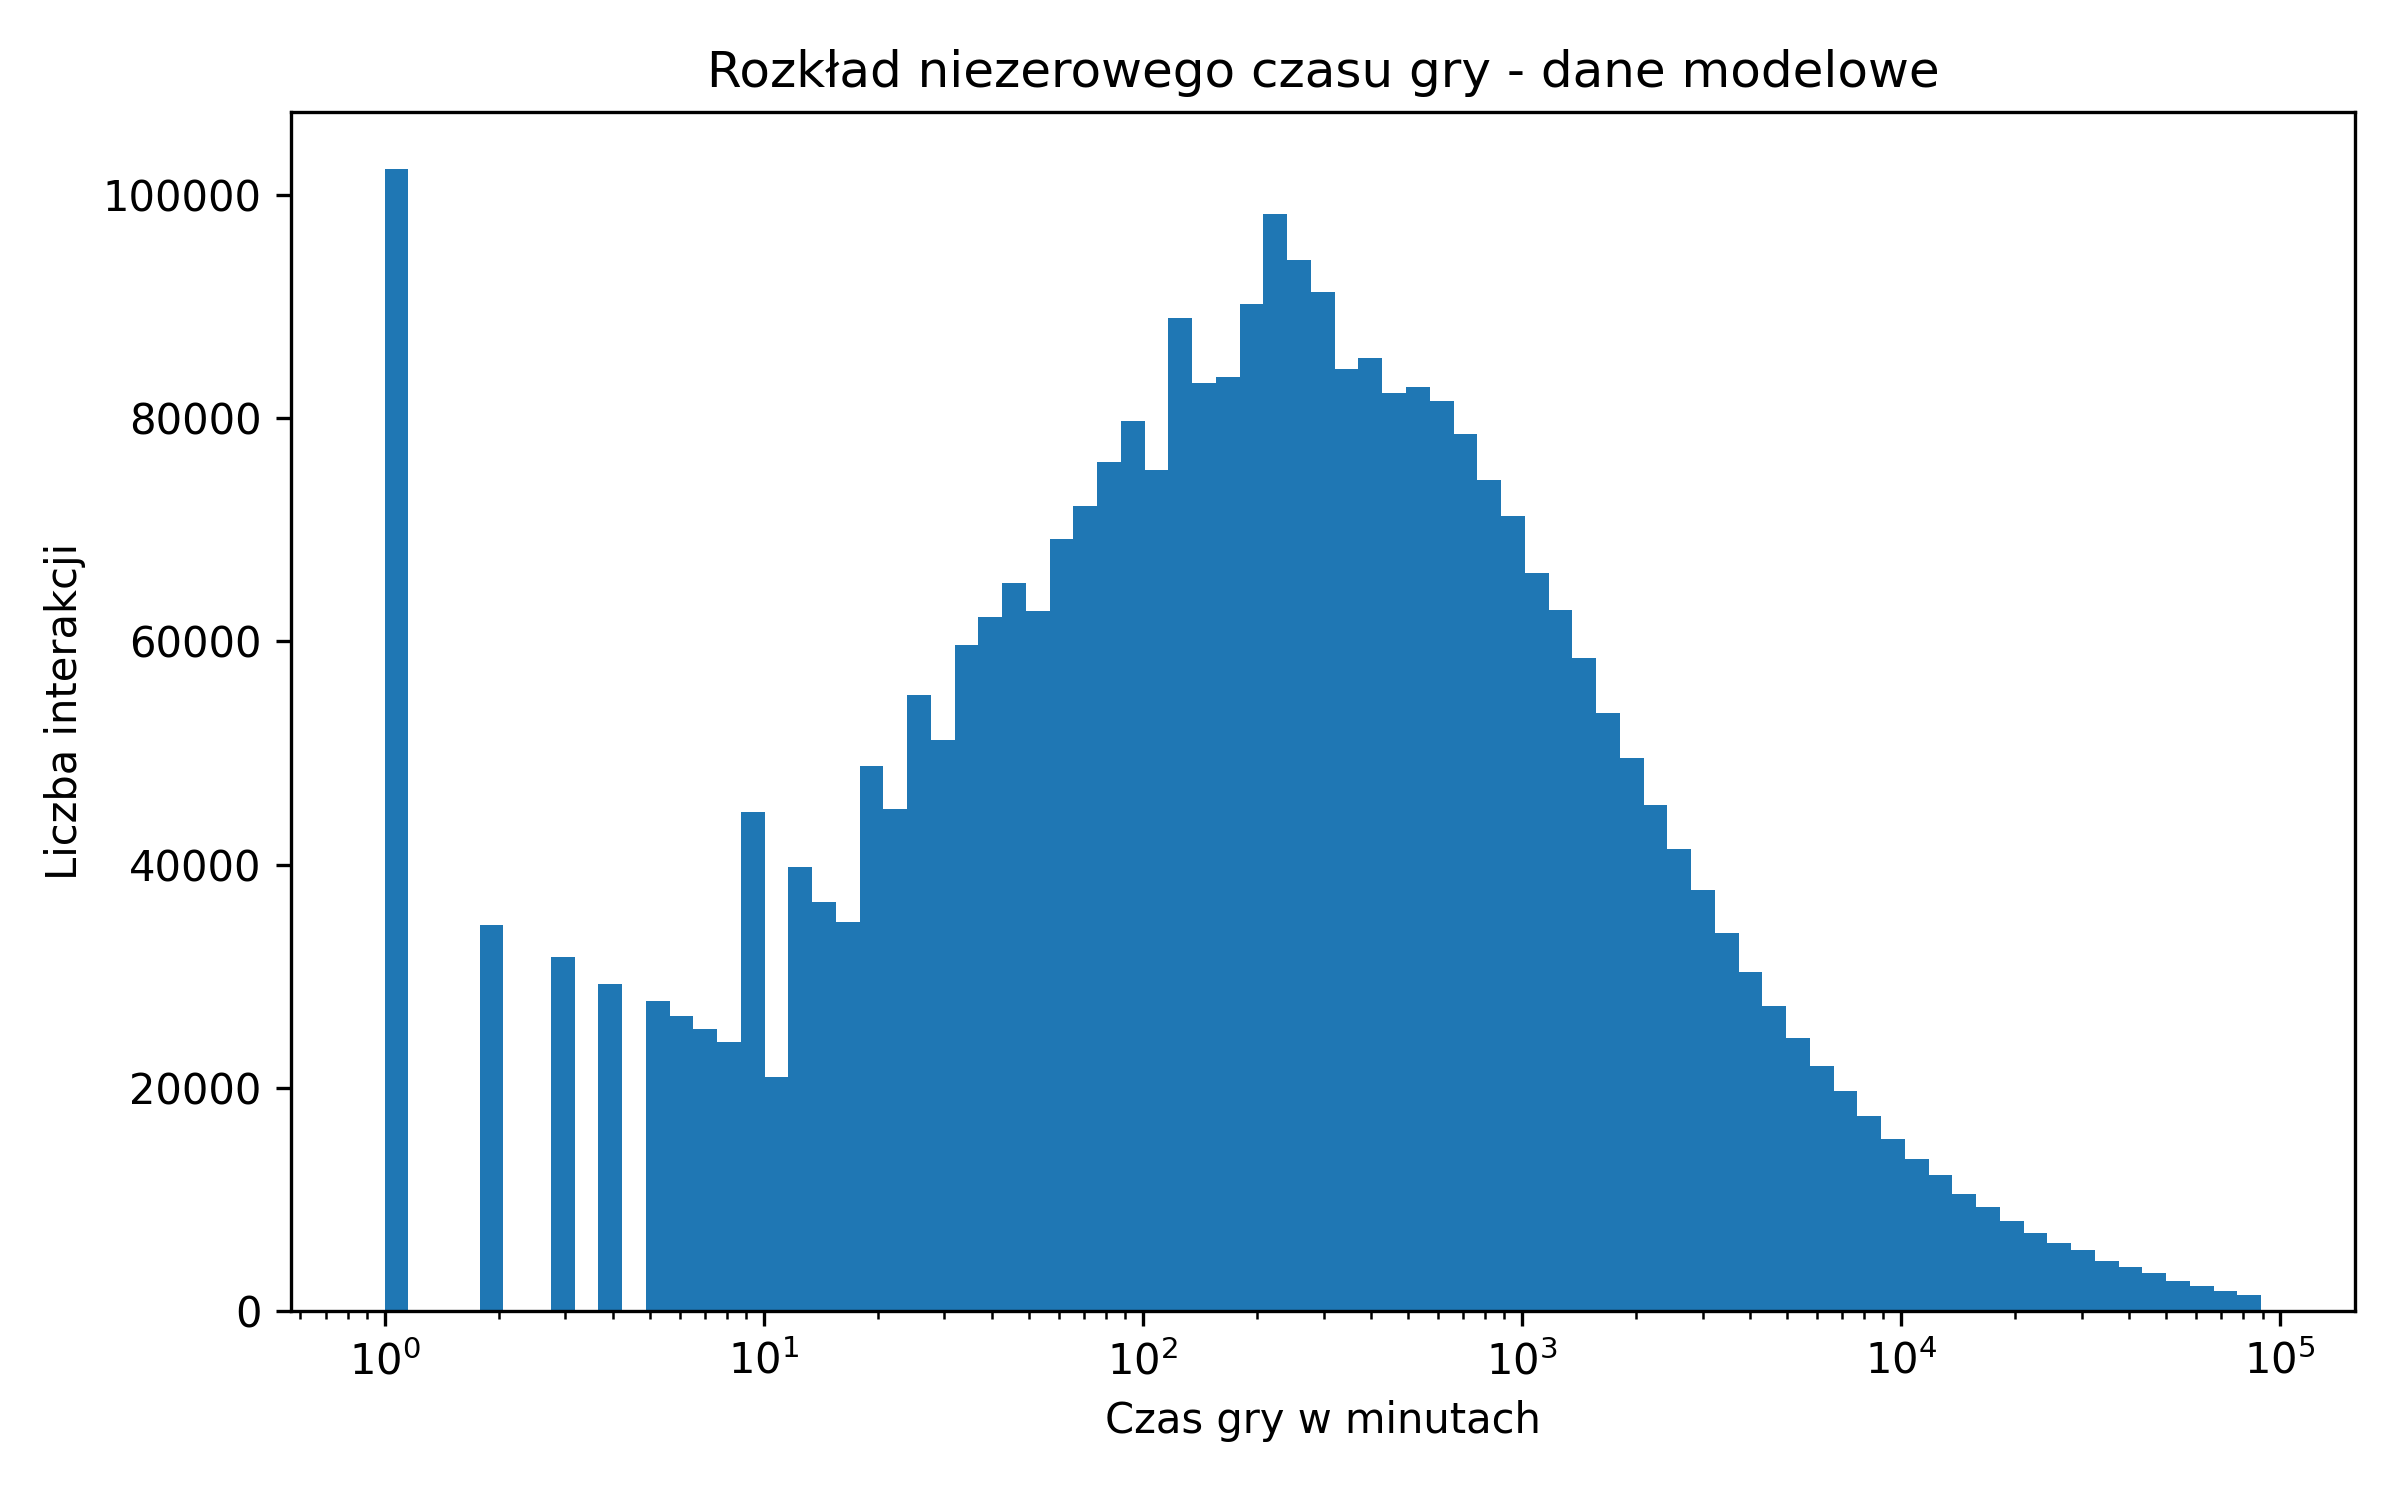
\includegraphics[width=0.9\textwidth]{figures/eda/filtered/filtered_positive_playtime_logscale_hist.png}
    \caption{Rozkład dodatniego czasu gry w skali logarytmicznej w przygotowanym zbiorze}
    \label{fig:filtered_positive_playtime_hist}
\end{figure}

Skośność rozkładu czasu gry stanowi przesłankę do rozważenia funkcji pewności o~spowolnionym wzroście. Liniowe potraktowanie zmiennej \texttt{playtime\_forever} nadawałoby bardzo dużą wagę skrajnym obserwacjom, przez co mogłoby zaburzać proces uczenia modelu. Natomiast sam fakt obecności gry w bibliotece pozostaje istotną informacją nawet wtedy, gdy czas gry jest równy zero. Z tego powodu w pracy zbadane zostały funkcje pewności ograniczające wpływ skrajnych wartości zmiennej odpowiadającej za czas gry oraz nadające obserwacjom z zerowym czasem gry zwiększoną wagę bazową. Definicje poszczególnych funkcji pewności przedstawiono w~podrozdziale~\ref{sec:porownywane-modele}.

\section{Aktywność użytkowników i popularność gier}

\subsection{Aktywność użytkowników}

Rozkład liczby interakcji przypadających na użytkownika jest prawostronnie
skośny, co przedstawiono na rysunku~\ref{fig:filtered_user_interaction_counts}. Widoczne skupienie przy niskich wartościach oraz długi ogon pokazują, że zbiór łączy dużą liczbę użytkowników o umiarkowanej aktywności z niewielką grupą kont posiadających bardzo rozbudowane biblioteki. W przygotowanym zbiorze średnia liczba interakcji na użytkownika wynosiła 81{,}54, podczas gdy mediana była równa 48. Pełne zestawienie statystyk rozkładu przedstawiono w~tabeli~\ref{tab:user_item_activity_stats}.

\begin{table}[htbp]
\centering
\caption{Rozkład liczby interakcji użytkowników i popularności gier w przygotowanym zbiorze}
\label{tab:user_item_activity_stats}
\begin{tabular}{lrr}
\toprule
Statystyka & \multicolumn{1}{c}{Na użytkownika} & \multicolumn{1}{c}{Na grę} \\
\midrule
Średnia & 81{,}54 & 558{,}01 \\
Mediana & 48 & 71 \\
95. percentyl & 251 & 2\,515{,}05 \\
99. percentyl & 518{,}57 & 8\,811{,}84 \\
Maksimum & 7\,337 & 45\,699 \\
\bottomrule
\end{tabular}
\end{table}

\begin{figure}[htbp]
    \centering
    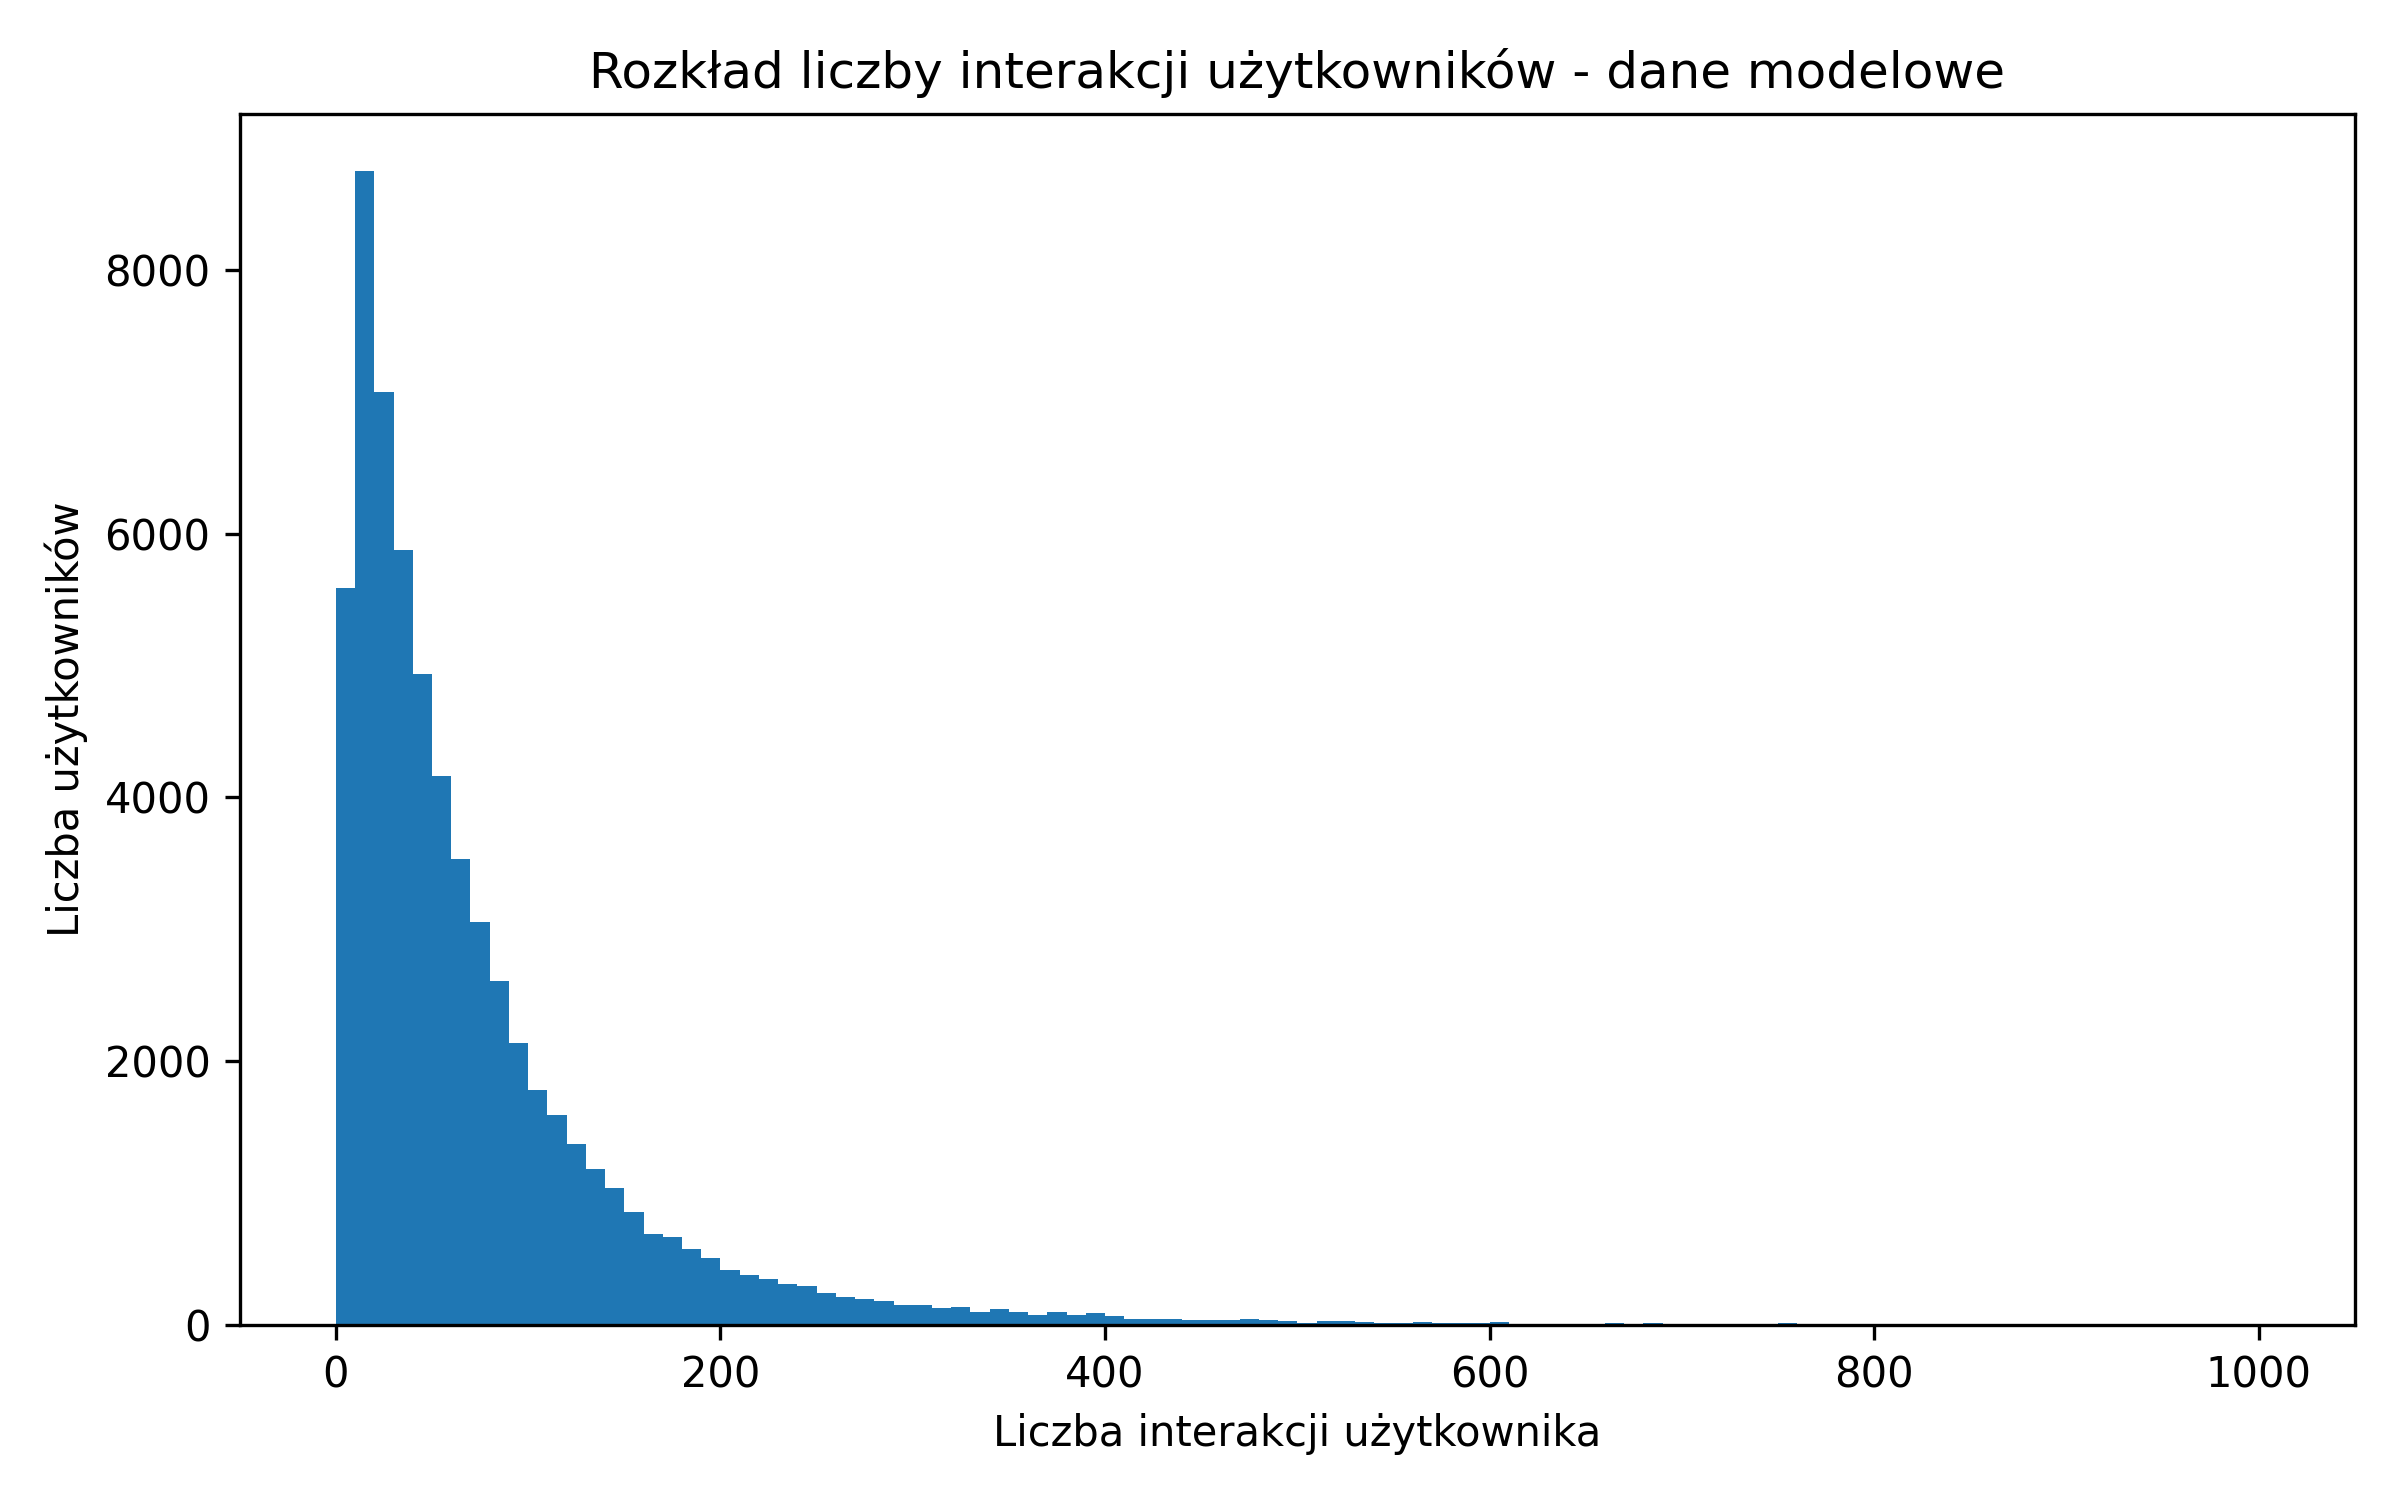
\includegraphics[width=0.9\textwidth]{../results/eda/figures_filtered/filtered_user_interaction_counts_hist.png}
    \caption{Rozkład liczby interakcji przypadających na użytkownika w przygotowanym zbiorze danych}
    \label{fig:filtered_user_interaction_counts}
\end{figure}

\subsection{Popularność gier}

Jeszcze większe zróżnicowanie widać po stronie gier. Mediana liczby interakcji przypadających na grę wynosiła 71, podczas gdy średnia była równa 558{,}01. Wynika stąd, że większość gier występowała w~bibliotekach stosunkowo małej liczby użytkowników, natomiast niewielka grupa najpopularniejszych tytułów odpowiadała za bardzo dużą część wszystkich interakcji.

Koncentrację popularności przedstawiono na rysunku~\ref{fig:filtered_item_popularity_concentration}. Najpopularniejszy 1\% gier odpowiadał za około 27{,}16\% wszystkich interakcji, najpopularniejsze 5\% za 59{,}55\%, a najpopularniejsze 10\% za 74{,}71\%.

\begin{figure}[htbp]
    \centering
    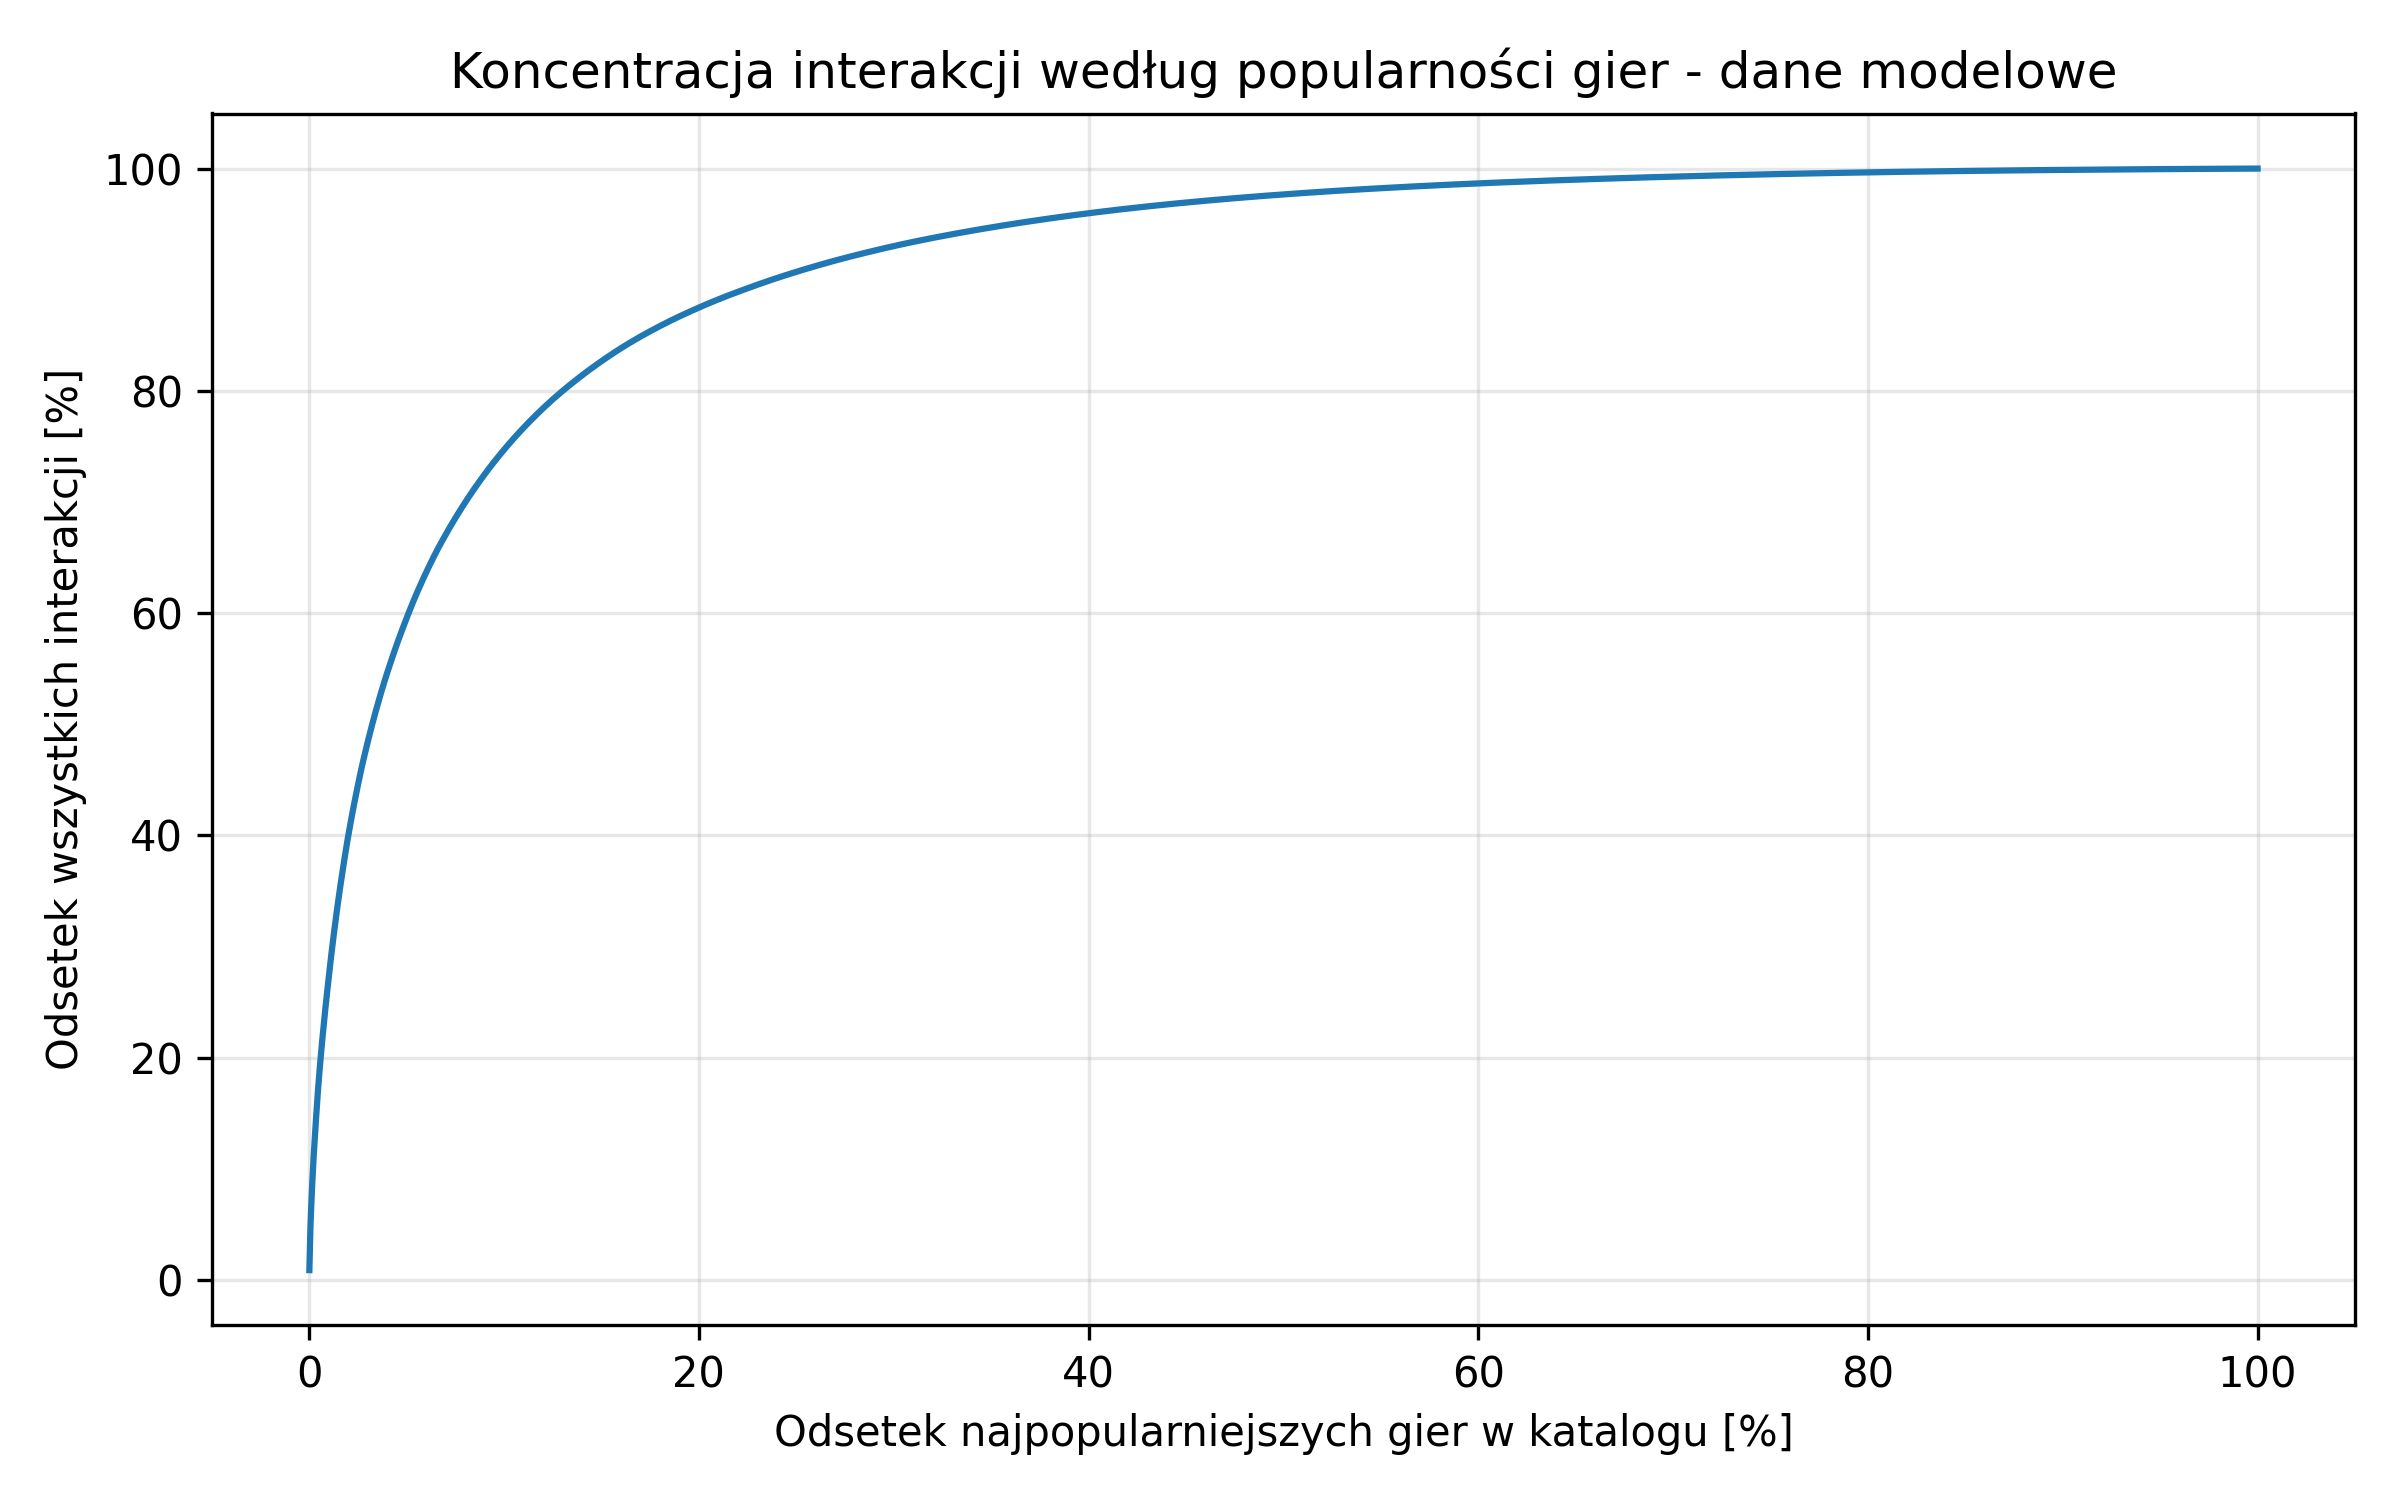
\includegraphics[width=0.9\textwidth]{../results/eda/figures_filtered/filtered_item_popularity_concentration.png}
    \caption{Koncentracja interakcji według popularności gier w przygotowanym zbiorze danych}
    \label{fig:filtered_item_popularity_concentration}
\end{figure}

Dodatkową ilustracją tej nierównomierności jest zestawienie najpopularniejszych gier przedstawione na rysunku~\ref{fig:filtered_top_games}. Wśród tytułów o największej liczbie interakcji znajdują się przede wszystkim bardzo popularne gry wieloosobowe oraz darmowe produkcje obecne w bibliotekach dużej liczby użytkowników. Obecność takich pozycji pokazuje, że prosty model oparty wyłącznie na popularności mógłby generować pozornie atrakcyjne rekomendacje, ale jednocześnie silnie ograniczałby różnorodność katalogu.

\begin{figure}[htbp]
    \centering
    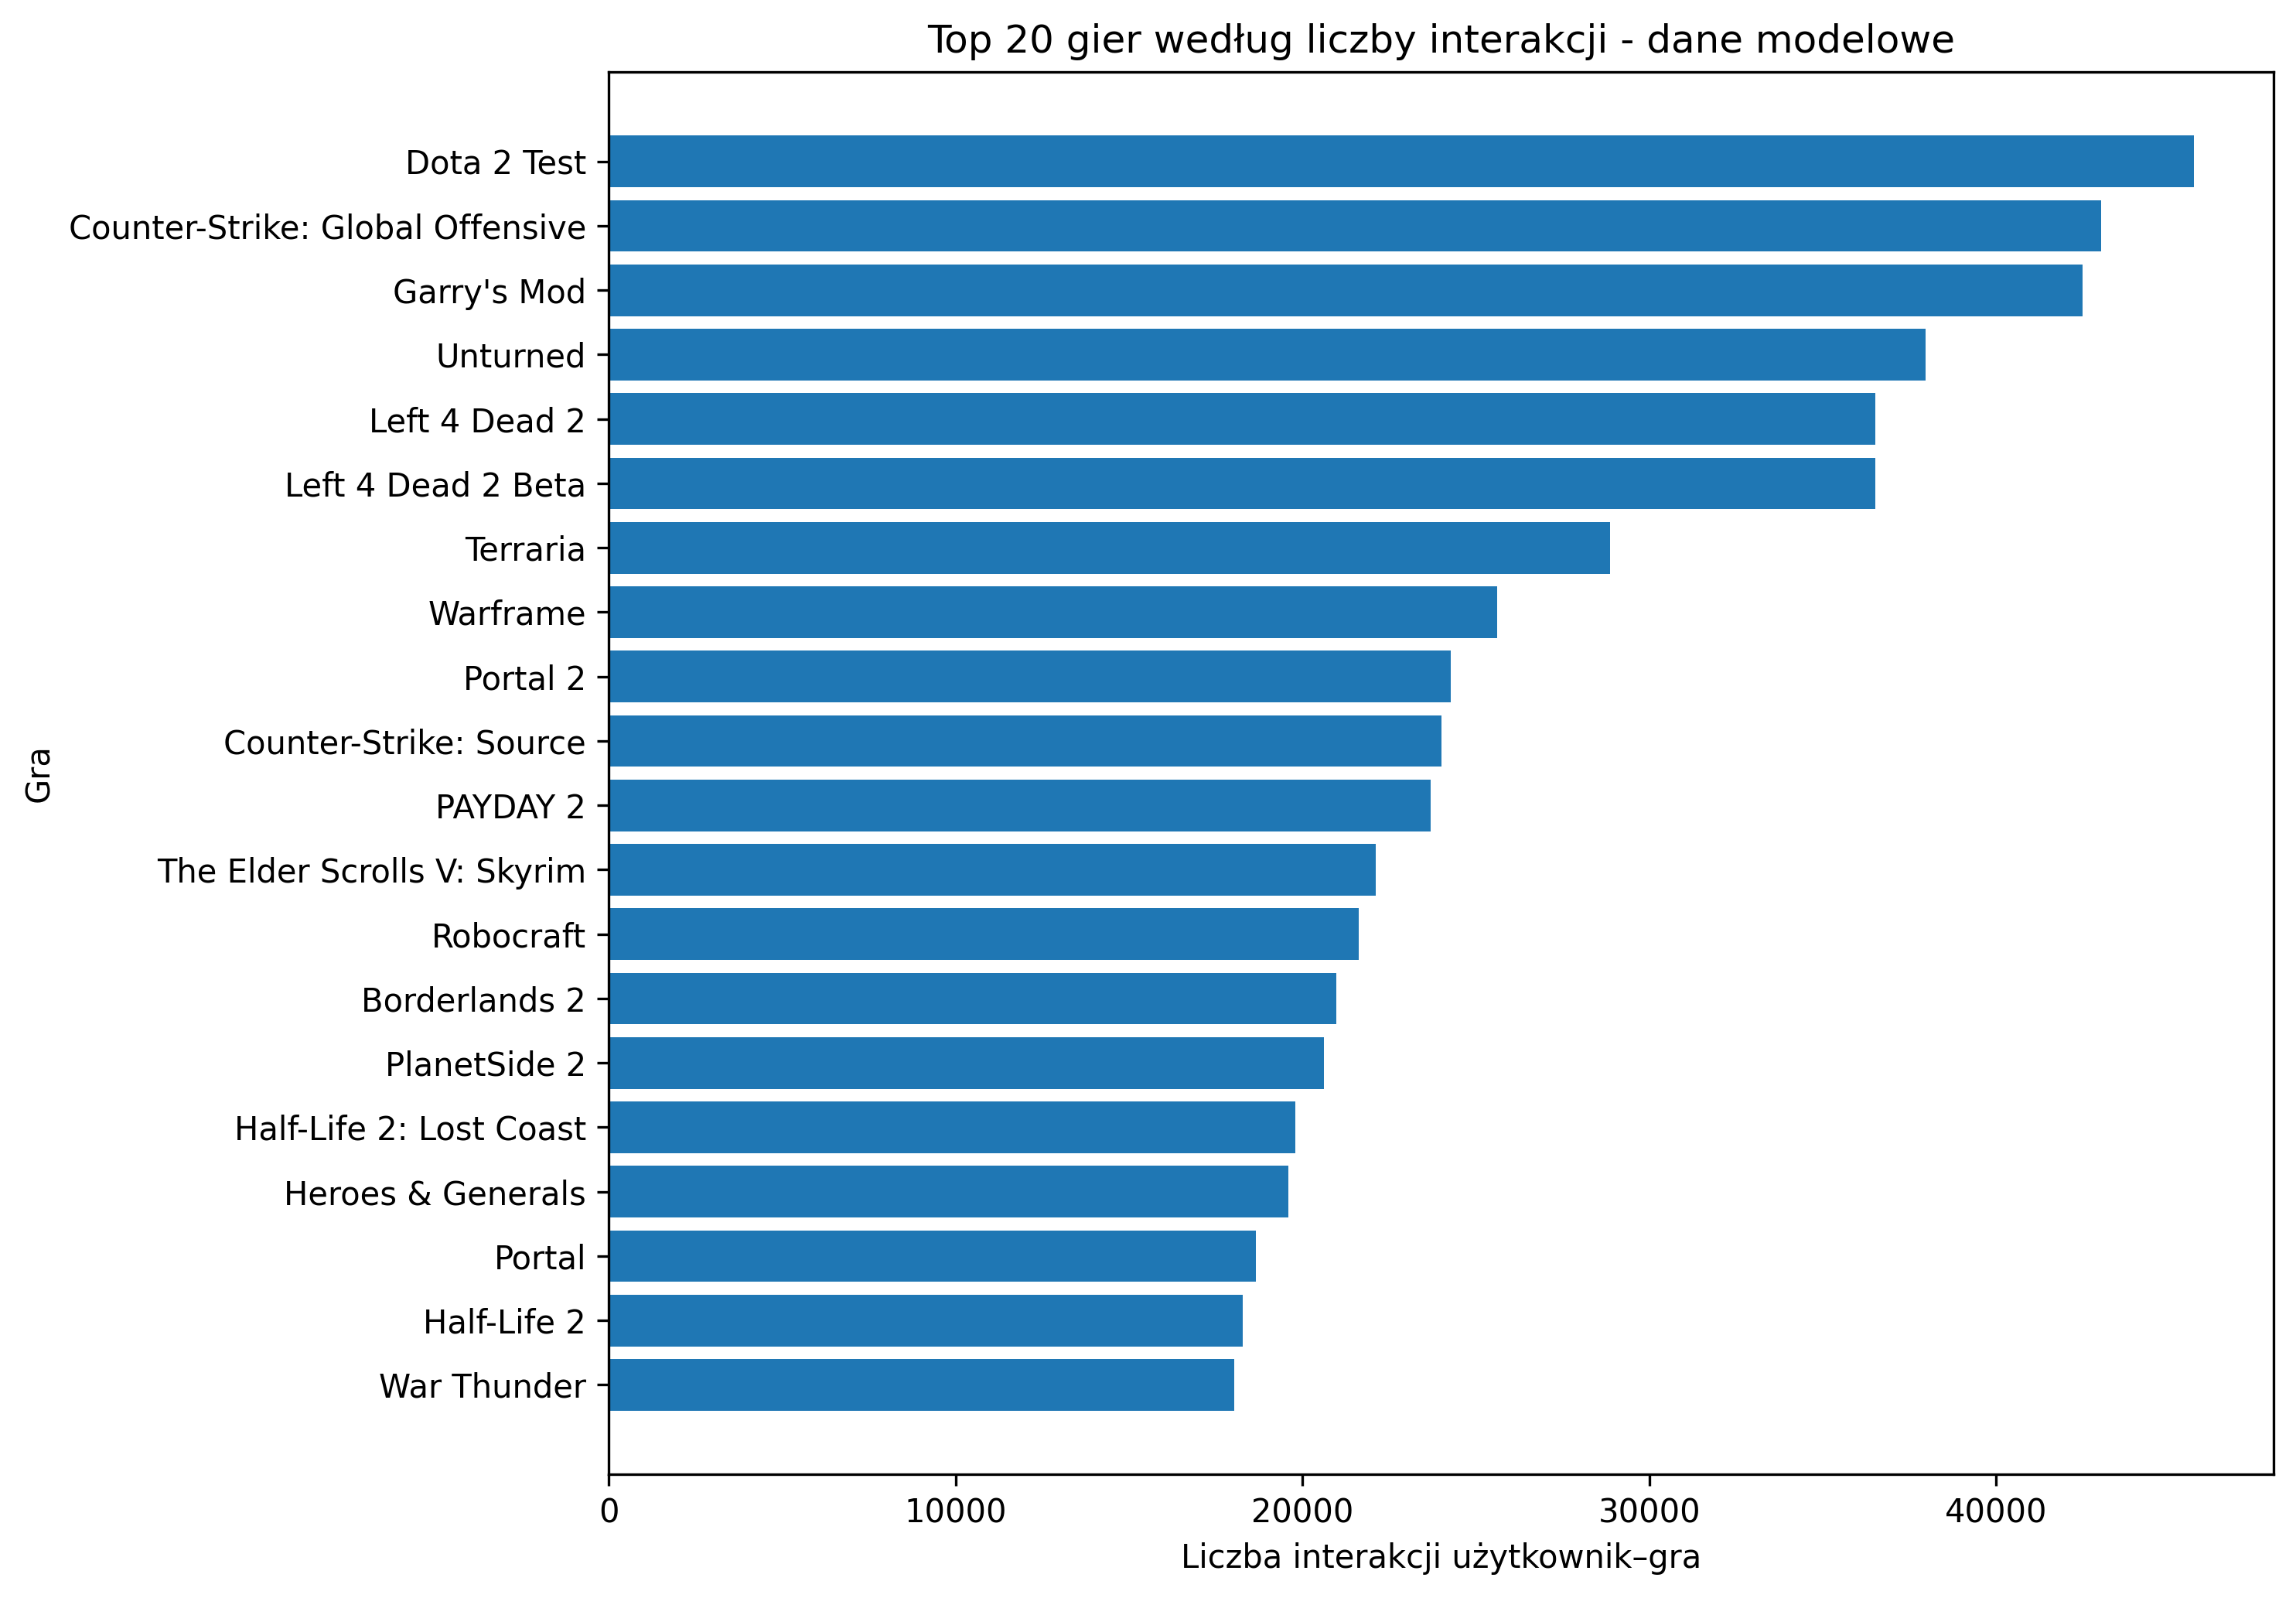
\includegraphics[width=0.9\textwidth]{../results/eda/figures_filtered/filtered_top_20_games_by_interactions.png}
    \caption{Dwadzieścia najpopularniejszych gier według liczby interakcji w przygotowanym zbiorze danych}
    \label{fig:filtered_top_games}
\end{figure}

Zaobserwowana koncentracja popularności ma znaczenie dla interpretacji późniejszych wyników eksperymentalnych. Modele rekomendacyjne mogą osiągać dobrą trafność, często rekomendując najpopularniejsze tytuły, ale takie zachowanie prowadzi do niskiego pokrycia katalogu i silnego obciążenia rekomendacji popularnością. Z tego powodu w dalszej części pracy, obok metryk trafności rankingowej, analizowane są również miary pokrycia katalogu oraz popularności rekomendowanych gier~\cite{kaminskas2016diversity,abdollahpouri2019unfairness}.

\section{Wnioski z analizy eksploracyjnej}

Najważniejsze cechy analizowanego zbioru danych, które bezpośrednio wpłynęły na przyjętą metodologię badawczą, to silnie prawostronnie skośny rozkład czasu gry użytkowników oraz wyraźna koncentracja popularności gier. Rozkład zmiennej \texttt{playtime\_forever} charakteryzuje się długim ogonem, co wymaga odpowiedniego przekształcenia tej zmiennej w wagę pewności wykorzystywaną w modelu. Z kolei nierównomierny rozkład popularności gier oznacza, że niewielka część katalogu generuje znaczną część interakcji, co należy uwzględnić w ocenie jakości rekomendacji poprzez analizę miar pokrycia katalogu oraz obciążenia popularnością.

Kolejnym istotnym aspektem jest rola obserwacji z wartością \texttt{playtime\_forever = 0}, które odmiennie od dominującego w literaturze trendu ich usuwania~\cite{bunga2021implicit, cheuque2019steam} zostały zachowane w procesie uczenia jako istotny sygnał behawioralny. Ich uwzględnienie wymaga funkcji pewności, która przypisuje takim obserwacjom wagę podwyższoną względem wartości domyślnej. Osobną kwestią pozostaje, czy jednoczesne spowolnienie przyrostu wagi dla rosnących czasów gry poprawia jakość rekomendacji. Odpowiedź na to pytanie przedstawiono w~dalszej części pracy.
\chapter{Metodyka eksperymentów}
\label{chap:metodologia}

\section{Przygotowanie danych}

Przed właściwym procesem trenowania modeli dane zostały poddane wstępnej obróbce. W analizowanym zbiorze nie występowały braki danych, więc ich filtracja nie była konieczna. Ze względu na obecność wartości odstających zmiennej \texttt{playtime\_forever} zdecydowano się na ograniczenie jej wartości do $120\,000$ minut, co odpowiada 2\,000~godzin i~w~przybliżeniu percentylowi 99{,}97 rozkładu w~zbiorze danych. Obserwacje powyżej tej granicy zostały zastąpione wartością $120\,000$. Przyjęty próg ogranicza wpływ wartości skrajnych i potencjalnych błędów pomiarowych, przy jednoczesnym zachowaniu sygnału o ekstremalnym zaangażowaniu użytkowników.

Usunięto gry przypisane do mniej niż pięciu użytkowników oraz użytkowników posiadających w~bibliotece mniej niż pięć gier. Miało to na celu zmniejszenie wpływu zimnego startu na wyniki modeli oraz umożliwienie późniejszego podziału danych na zbiory treningowy, walidacyjny i testowy, w sposób zapewniający, że każdy użytkownik pojawi się w każdym z tych zbiorów. Podejścia stosowane w~pracach wykorzystujących ten sam zbiór danych są wyraźnie bardziej restrykcyjne. Obejmują one usuwanie interakcji z~zerowym czasem gry oraz ograniczanie zbioru do najaktywniejszych użytkowników i~najpopularniejszych tytułów~\cite{bunga2021implicit,cheuque2019steam}. Zabiegi tego rodzaju zwiększają gęstość macierzy interakcji, jednak zawężają populację i~czynią zadanie ewaluacyjne mniej wymagającym. Szczegółowe zestawienie różnic wraz z~ich konsekwencjami dla porównywalności wyników przedstawiono w~podrozdziale~\ref{sec:porownanie-literatura}.

Zbiór po filtracji został podzielony na zbiory: treningowy, walidacyjny i testowy. Dla każdego użytkownika do zbioru testowego przypisano liczbę interakcji równą
$\left\lceil 0{,}1 \cdot n_u \right\rceil$,
gdzie $n_u$ oznacza liczbę interakcji danego użytkownika. Zastosowano zaokrąglenie w górę, aby zapewnić, że każdy użytkownik będzie miał co najmniej jedną interakcję w zbiorze testowym. Podział został przeprowadzony w sposób losowy ze względu na brak informacji o datach przypisania produktów do bibliotek użytkowników. Z pozostałej części danych, stanowiącej w przybliżeniu $90\%$ zbioru, wydzielono do zbioru walidacyjnego liczbę interakcji wyznaczoną analogicznie, czyli $\left\lceil 0{,}1 \cdot n_{u,\text{rem}} \right\rceil$, gdzie $n_{u,\text{rem}}$ oznacza pozostałą po pierwszym podziale liczbę interakcji użytkownika. Ostateczna struktura podziału danych wynosi zatem w przybliżeniu $81\%$ dla zbioru treningowego, $9\%$ dla walidacyjnego oraz $10\%$ dla testowego, co jest rozwiązaniem bardzo zbliżonym do proporcji stosowanych m.in. w pracach~\cite{wang2019neural, moscati2026networked} oraz standardowego podziału w bibliotece RecBole~\cite{recbole}. Na każdym etapie ustalono stałą wartość ziarna generatora liczb pseudolosowych, co zapewnia powtarzalność podziału danych.

\section{Porównywane modele}
\label{sec:porownywane-modele}

Porównano siedem modeli rekomendacyjnych, w tym pięć modeli implicit ALS z różnymi funkcjami pewności oraz model Bayesian Personalized Ranking, których implementacje pochodzą z biblioteki \texttt{implicit} w wersji 0.7.2~\cite{frederickson2022implicit}. Zastosowane funkcje pewności to:
\begin{itemize}
    \item $c_{ui} = 1 + \alpha r_{ui}$,
    \item $c_{ui} = 1 + \alpha \log(1 + r_{ui})$,
    \item $c_{ui} = 1 + \alpha \frac{\log(1 + r_{ui})}{1 + \log(1 + r_{ui})}$,
    \item $c_{ui} = 1 + \alpha \log(1 + r_{ui} + \beta) \cdot \mathbf{1}(p_{ui} = 1)$,
    \item $c_{ui} = 1 + \gamma \cdot \mathbf{1}(p_{ui} = 1)$,
\end{itemize}
gdzie $r_{ui}$ oznacza wartość zmiennej \texttt{playtime\_forever} dla użytkownika $u$ i gry $i$, a $\alpha$ stanowi skalar regulujący siłę wpływu czasu gry. Dla par niezaobserwowanych ($p_{ui} = 0$) waga pewności wynosi $c_{ui} = 1$, co w~przypadku dwóch ostatnich funkcji zapewnia wskaźnik $\mathbf{1}(p_{ui}=1)$. W~dalszej części pracy funkcje te przywoływane są w~postaci skróconej, z~pominięciem wskaźnika. Dwie pierwsze funkcje stanowią klasyczne sformułowania zaproponowane w pracy \cite{hu2008implicit}. 

Funkcje logarytmiczna z~saturacją oraz logarytmiczna z~przesunięciem $\beta$ są wariantami zaproponowanymi na potrzeby niniejszej pracy, opracowanymi na podstawie analizy rozkładu zmiennej \texttt{playtime\_forever} przedstawionej w~rozdziale~\ref{chap:eda}. Wariant stały odpowiada wzorowi $c_{ui} = 1 + \alpha r_{ui}$ zastosowanemu do zbinaryzowanego sygnału, w~którym $r_{ui}$ przyjmuje wartość $1$ dla każdej gry obecnej w~bibliotece.

Wartości funkcji pewności $c_{ui}$ wyznaczano dla par użytkownik--gra zapisanych w ramce danych. Następnie na ich podstawie, z wykorzystaniem biblioteki \texttt{scipy} w wersji 1.17.1, tworzono macierz rzadką przekazywaną do metody \texttt{fit()} modeli ALS. W przypadku modeli implicit ALS parametr \texttt{alpha} klasy \texttt{AlternatingLeastSquares} z biblioteki \texttt{implicit} pozostawiono równy $1$, ponieważ został on uwzględniony bezpośrednio podczas wyznaczania wartości $c_{ui}$. Ze względu na to, że każda funkcja pewności przyjmuje dla $r_{ui}=0$ wartość co najmniej $1$, podczas tworzenia macierzy rzadkiej nie została utracona żadna para użytkownik--gra obecna w zbiorze danych. Oznacza to, że również obserwacje z $\texttt{playtime\_forever}=0$ są uwzględniane jako obserwacje pozytywne.

Model Bayesian Personalized Ranking otrzymywał binarną macierz rzadką, w której każdej obserwowanej parze użytkownik--gra przypisano wartość $1$. Dzięki temu zarówno modele ALS, jak i BPR operowały na tym samym zbiorze obserwowanych par. W obu przypadkach pary użytkownik--gra nieobecne w zbiorze danych nie były traktowane jako obserwacje pozytywne.

Punkt odniesienia dla obu rodzin modeli stanowi rekomendacja oparta na popularności. Dla każdego użytkownika generuje ona listę $N$ tytułów o~największej liczbie użytkowników w~zbiorze treningowym, z~pominięciem pozycji już obecnych w~jego bibliotece. Jego uwzględnienie
pozwala ocenić, jaka część trafności modeli faktoryzacyjnych wykracza poza odtworzenie rozkładu popularności opisanego w~rozdziale~\ref{chap:eda}.

W szczególności, funkcja $c_{ui} = 1 + \alpha \log(1 + r_{ui} + \beta)$ została zaprojektowana w celu zmniejszenia wpływu szumu wynikającego z dużej liczby obserwacji o niskim czasie gry, przy jednoczesnym wprowadzeniu przesunięcia $\beta$. Pozwala ono nadawać obserwacjom z \texttt{playtime\_forever = 0} wagę pewności większą niż $1$, co jest traktowane w pracy jako wstępny sygnał zainteresowania użytkownika. Aby zweryfikować, czy ewentualna poprawa wyników wynika z połączonego efektu kompresji szumu i dodatkowej wagi bazowej, czy też wyłącznie z faktu przypisania wyższej ufności zerowym obserwacjom, wprowadzono dodatkowo funkcję $c_{ui} = 1 + \gamma$, gdzie $\gamma$ jest hiperparametrem. Aby uniknąć arbitralnego wyboru wartości, oba nowe hiperparametry, $\beta$ oraz $\gamma$, poddano procesowi optymalizacji.

\section{Strojenie hiperparametrów}

Proces strojenia hiperparametrów został przeprowadzony na podstawie zbioru walidacyjnego. Celem była optymalizacja \ndcg{} dla każdego z modeli. Metryka ta została wybrana ze względu na jej własności opisane w podrozdziale~\ref{subsec:ndcg}. Procedura miała charakter dwuetapowy. Najpierw przeprowadzono szerokie przeszukanie siatkowe dla wszystkich modeli, aby znaleźć przybliżony zakres najlepszych wartości hiperparametrów, a następnie dokładnie przeszukano ten zakres z~wykorzystaniem biblioteki Optuna~\cite{akiba2019optuna}, stosując estymator drzewiasty Parzena. W przypadku modeli implicit ALS strojenie obejmowało hiperparametry $\alpha$, $\beta$ i $\gamma$ odpowiedzialne za wagę pewności, liczbę czynników ukrytych $f$ oraz siłę regularyzacji $\lambda$. Liczba iteracji algorytmu ALS została ustalona na 30, ze względu na brak istotnej poprawy wyników przy większej liczbie iteracji podczas wstępnego przeszukiwania siatkowego. Natomiast dla modelu BPR strojenie obejmowało $f$, $\lambda_\Theta$, liczbę iteracji oraz długość kroku $\eta$. W przypadku modelu popularnościowego nie przeprowadzano strojenia ze względu na brak hiperparametrów. Dla każdego z optymalizowanych modeli przeprowadzono 150 prób algorytmu w jednej serii. Aby wykluczyć ryzyko znalezienia nie w pełni optymalnych rozwiązań, po każdej serii oceniano stabilność metryki celowej oraz stopień skupienia uzyskanych hiperparametrów wokół znalezionego optimum. W sytuacjach, gdy najlepsze próby wykazywały dużą zmienność wartości hiperparametrów lub gdy znaleziona kombinacja znajdowała się na granicy przeszukiwanego przedziału, procedurę powtarzano z rozszerzonym lub przesuniętym zakresem aż do uzyskania spójnych wyników. Każdy etap przeprowadzono z ustalonym ziarnem generatora liczb pseudolosowych, co gwarantuje reprodukowalność procesu optymalizacji.


\section{Finalna ewaluacja testowa}

Po wybraniu optymalnych wartości hiperparametrów dla każdego z~modeli obliczono odchylenie standardowe metryk dla pięciu losowych podziałów na zbiór treningowy i~walidacyjny, w~celu sprawdzenia stabilności wyników ze względu na losowość podziału danych. Następnie modele wytrenowano ponownie na połączonym zbiorze treningowym i~walidacyjnym, z~hiperparametrami wybranymi na podstawie zbioru walidacyjnego, po czym poddano je ewaluacji z~użyciem miar trafności:  precyzji, pełności oraz $\text{NDCG}$, a~także miar wykraczających poza trafność: pokrycia katalogu, różnorodności wewnątrzlistowej ($\text{ILD}$) oraz różnicy w~popularności rekomendacji ($\Delta\text{GAP}$). Każdą z~metryk obliczono dla listy rekomendacji o~długości 10, co stanowi rozwiązanie powszechnie przyjmowane w~literaturze~\cite{he2017neural,rendle2020neural}, a~następnie uśredniono po wszystkich użytkownikach. Ewaluację powtórzono pięciokrotnie przy stałym podziale danych i~zmiennym ziarnie inicjalizacji modelu, co pozwala oddzielić zmienność wynikającą z~podziału danych od zmienności wynikającej z~inicjalizacji; dla uzyskanych wartości wyznaczono średnią oraz odchylenie standardowe. Wyjątek stanowi różnorodność wewnątrzlistowa, którą ze względu na koszt obliczeniowy wyznaczono dla pojedynczego uruchomienia i~pominięto w~analizie stabilności. Odwzorowanie identyfikatorów zbioru testowego na indeksy wyznaczone na zbiorze treningowym powoduje pominięcie interakcji dotyczących użytkowników lub gier nieobecnych w~zbiorze treningowym. W~przeprowadzonym eksperymencie sytuacja taka nie wystąpiła. Zatem wszystkie 541\,231 interakcji testowych zostały uwzględnione przy wyznaczaniu metryk.

Metrykę \ndcg{} wyznaczono dodatkowo indywidualnie dla każdego użytkownika, uśredniając wartości uzyskane w~pięciu uruchomieniach. Tak przygotowane wartości posłużyły do przeprowadzenia testu Wilcoxona dla par obserwacji we wszystkich dziesięciu porównaniach parowych między wariantami funkcji pewności, z~korektą Holma-Bonferroniego na wielokrotne testowanie. Ze względu na dużą liczbę użytkowników, przy której istotność statystyczną osiągają również różnice o~niewielkiej skali, dla każdej pary wariantów wyznaczono ponadto medianę oraz średnią sparowanej różnicy \ndcg{} wraz z~95-procentowym przedziałem ufności. Przedziały oszacowano za pomocą nieparametrycznego bootstrapu dla prób zależnych na poziomie użytkownika. W~każdym z~5\,000 powtórzeń losowano ze zwracaniem $n=62\,944$ użytkowników, a~następnie dla każdego powtórzenia obliczano średnią sparowanej różnicy \ndcg{} na podstawie tych samych wylosowanych użytkowników. Wspólny zestaw indeksów bootstrapowych był wykorzystywany dla wszystkich porównań, dzięki czemu zachowano strukturę zależności między wynikami uzyskiwanymi przez tego samego użytkownika dla poszczególnych wariantów. Przedział ufności wyznaczano metodą percentylową, przyjmując 2{,}5. i~97{,}5. percentyl rozkładu wartości uzyskanych w~bootstrapie jako odpowiednio jego dolną i~górną granicę.

\section{Analiza wrażliwości na \texorpdfstring{$\alpha$}{alpha}, \texorpdfstring{$\beta$}{beta} i \texorpdfstring{$\gamma$}{gamma}}

Ze względu na szczególne zainteresowanie wpływem wag pewności na jakość rekomendacji, przeprowadzono dodatkową analizę parametrów odpowiedzialnych za ich skalowanie i przesunięcie, czyli $\alpha$, $\beta$ oraz $\gamma$. W tym celu dla każdej funkcji pewności w modelach implicit ALS przeprowadzono eksperymenty, w których obliczono \ndcg{} dla 25 wartości hiperparametru $\alpha$ w równych odstępach na siatce logarytmicznej wokół optymalnej wartości znalezionej w procesie strojenia. Analogiczne badanie wrażliwości przeprowadzono dla 40 wartości parametru $\beta$ w~zakresie od $1$ do $10^{6}$ oraz 40 wartości parametru $\gamma$
w~zakresie od $10^{-3}$ do $10^{4}$, w~obu przypadkach na siatce logarytmicznej. W podrozdziale~\ref{sec:confidence_analysis} przedstawiono również dodatkowe wykresy przedstawiające zależność funkcji pewności od zmiennej \texttt{playtime\_forever} oraz wyznaczono jej efektywny zakres dla poszczególnych modeli implicit ALS. Pozwoliło to na lepsze zrozumienie, w jaki sposób zastosowane przekształcenia wpływają na proces uczenia modeli.


\section{Ograniczenia metodologii}

Przeprowadzone badanie ma ograniczenia, które należy uwzględnić przy
interpretacji wyników.

\begin{itemize}
    \item \textbf{Jeden zbiór danych.} Eksperyment zrealizowano wyłącznie na
    danych platformy Steam. Uogólnienie wniosków wymagałoby powtórzenia go na
    zbiorach pochodzących z~innych platform, w~których sygnał intensywności
    interakcji ma odmienny charakter.

    \item \textbf{Postać sygnału.} Zmienna \texttt{playtime\_forever} agreguje
    czas gry przez cały okres posiadania tytułu, nie oddając ani intensywności,
    ani aktualności rozgrywki. Formułowane wnioski dotyczą tej konkretnej
    postaci sygnału i~nie przenoszą się automatycznie na miary uwzględniające
    jego rozkład w~czasie.

    \item \textbf{Brak wymiaru czasowego.} Zbiór nie zawiera dat przypisania
    gier do bibliotek, co uniemożliwiło podział danych w~porządku
    chronologicznym oraz uwzględnienie zmiany preferencji użytkowników w~czasie.

    \item \textbf{Ewaluacja offline.} Ocena została przeprowadzona wyłącznie na
    danych historycznych, bez testu A/B. Nie pozwala to zweryfikować, czy
    obserwowane różnice przekładają się na rzeczywiste zachowania użytkowników.

    \item \textbf{Brak podziału na grupy użytkowników.} Ewaluację
    przeprowadzono na całej populacji, bez rozróżnienia według liczby
    interakcji. Podział taki mógłby ujawnić różnice w~jakości rekomendacji dla
    użytkowników o~różnym poziomie aktywności.

    \item \textbf{Uproszczenia analizy wrażliwości.} Ze względu na koszt
    obliczeniowy podczas badania wpływu $\alpha$, $\beta$ i~$\gamma$ pozostałe
    hiperparametry utrzymano na stałym poziomie, wyznaczonym na podstawie
    najlepszego modelu w~danej rodzinie. Wyniki opisują zatem lokalne otoczenie
    znalezionego optimum.
\end{itemize}
\chapter{Wyniki eksperymentów}

\section{Wyniki strojenia hiperparametrów}

Wyniki strojenia hiperparametrów dla każdego z modeli implicit ALS zostały przedstawione w tabeli~\ref{tab:hiperparametry-als}. Zgodnie z~ustaleniami przedstawionymi w~rozdziale~\ref{chap:metodologia}, liczba iteracji dla wszystkich wariantów ALS wynosi 30.

\begin{table}[htbp]
\centering
\caption{Najlepsze hiperparametry wariantów ALS wybrane na zbiorze walidacyjnym}
\label{tab:hiperparametry-als}
\begin{tabular}{lrrrrr}
\toprule
Wariant & $f$ & $\alpha$ & $\beta$ / $\gamma$ & $\lambda$ & \ndcg{} \\
\midrule
Liniowa & $80$ & $9{,}948\cdot 10^{-7}$ & --- & $0{,}003588$ & $0{,}249$\\
Logarytmiczna & $24$ & $0{,}000571$ & --- & $0{,}130920$ & $0{,}261$\\
Logarytmiczna z saturacją & $24$ & $0{,}024390$ & --- & $0{,}169714$ & $0{,}261$\\
Logarytmiczna z przesunięciem $\beta$ & $48$ & $0{,}389185$ & $108{,}284$ & $0{,}010565$ & $0{,}275$\\
Stała & $48$ & --- & $2{,}364$ & $0{,}057607$ & $0{,}280$\\
\bottomrule
\end{tabular}
\caption*{\footnotesize Kolumna $\beta$ / $\gamma$ zawiera parametr dodatkowy właściwy dla danego wariantu.
Źródło: opracowanie własne na podstawie wyników optymalizacji hiperparametrów.}
\end{table}

Warto zwrócić szczególną uwagę na niskie wartości parametru $\alpha$ odpowiadającego za skalowanie wagi pozytywnych interakcji. Jako standardową wartość tego hiperparametru zwykle przyjmuje się 1 \cite{sparkals,frederickson2022implicit}, a przeszukanie przeprowadza się wśród większych wartości w celu zróżnicowania długich interakcji od ich braku. Konsekwencją tego jest bardzo małe wykorzystanie potencjalnych informacji o preferencjach zawartych w długości czasu gry. Taki wynik był spodziewany w przypadku liniowego przekształcenia ze względu na przypisywanie ogromnych wag dla obserwacji z długiego ogona. Klasycznym rozwiązaniem tego problemu jest zastosowanie logarytmu, jednak pomimo poprawy \ndcg{} $\alpha$ nadal pozostała mała. Z tego powodu zdecydowano się na zastosowanie przekształcenia $c_{ui} = 1 + \alpha \frac{\log(1 + r_{ui})}{1 + \log(1 + r_{ui})}$ ograniczającego wartości zmiennej przed skalowaniem do przedziału $[0, 1)$. Nie miało to jednak znaczącego wpływu na metrykę \ndcg{} na zbiorze walidacyjnym, a dodatkowe eksperymenty pokazały marginalność różnic między tymi modelami. Na podstawie wyników poprzednich eksperymentów sformułowano hipotezę, że niskie wartości \texttt{playtime\_forever} wprowadzały znaczny szum do modeli stosujących logarytmiczne przekształcenia, co w efekcie zmuszało do doboru niewielkich $\alpha$ w procesie optymalizacji hiperparametrów. W celu zniwelowania tego zjawiska zastosowano przekształcenie $c_{ui} = 1 + \alpha \log(1 + r_{ui} + \beta)$, w którym przesunięcie $\beta$ podnosi pewność interakcji o zerowym czasie gry i jednocześnie kompresuje różnice między pozostałymi obserwacjami. W procesie optymalizacji $\beta$ została ustalona na wartość 108,284, co przy medianie czasu gry wynoszącej 35 minut oznacza, że dla znacznej części zbioru przekształcenie działa w obszarze bliskim stałemu.

Ta obserwacja doprowadziła do sformułowania pytania o brak wartości dodanej płynącej z monotonicznego uwzględnienia zmiennej \texttt{playtime\_forever}. W takim przypadku koniecznym punktem odniesienia jest przekształcenie całkowicie ignorujące czas gry. W tym celu wprowadzono wariant graniczny $c_{ui} = 1 + \gamma$, w którym wszystkie zaobserwowane interakcje otrzymują identyczną wagę, a jedynym strojonym parametrem pozostaje jej globalna wartość. Wariant ten osiągnął najwyższą wartość \ndcg{} na zbiorze walidacyjnym spośród wszystkich rozważanych funkcji pewności, przy $\gamma$ równym 2,364. Wynik ten wskazuje, że obserwowane wcześniej poprawy nie wynikały z lepszego odwzorowania siły preferencji, lecz ze zmniejszającego się wpływu zmiennej \texttt{playtime\_forever} na proces uczenia.

Należy przy tym podkreślić, że porównywane warianty dostrojono niezależnie, przez co różnią się nie tylko postacią funkcji pewności, lecz również liczbą czynników ukrytych oraz siłą regularyzacji. Przedstawione zestawienie pozwala zatem wnioskować o tym, który wariant po dostrojeniu prowadzi do najlepszych rekomendacji, nie zaś o izolowanym wpływie samego przekształcenia sygnału.

W celu lepszego zobrazowania wpływu omawianych hiperparametrów na jakość rekomendacji wygenerowano wykresy~\ref{fig:wrazliwosc_ndcg_vs_alpha}, \ref{fig:wrazliwosc_log_beta_ndcg_vs_beta} oraz~\ref{fig:wrazliwosc_ndcg_vs_gamma}, przedstawiające zależność \ndcg{} od wartości odpowiednio $\alpha$, $\beta$ i $\gamma$ w otoczeniu znalezionych wartości optymalnych.

\begin{figure}[htbp]
    \centering
    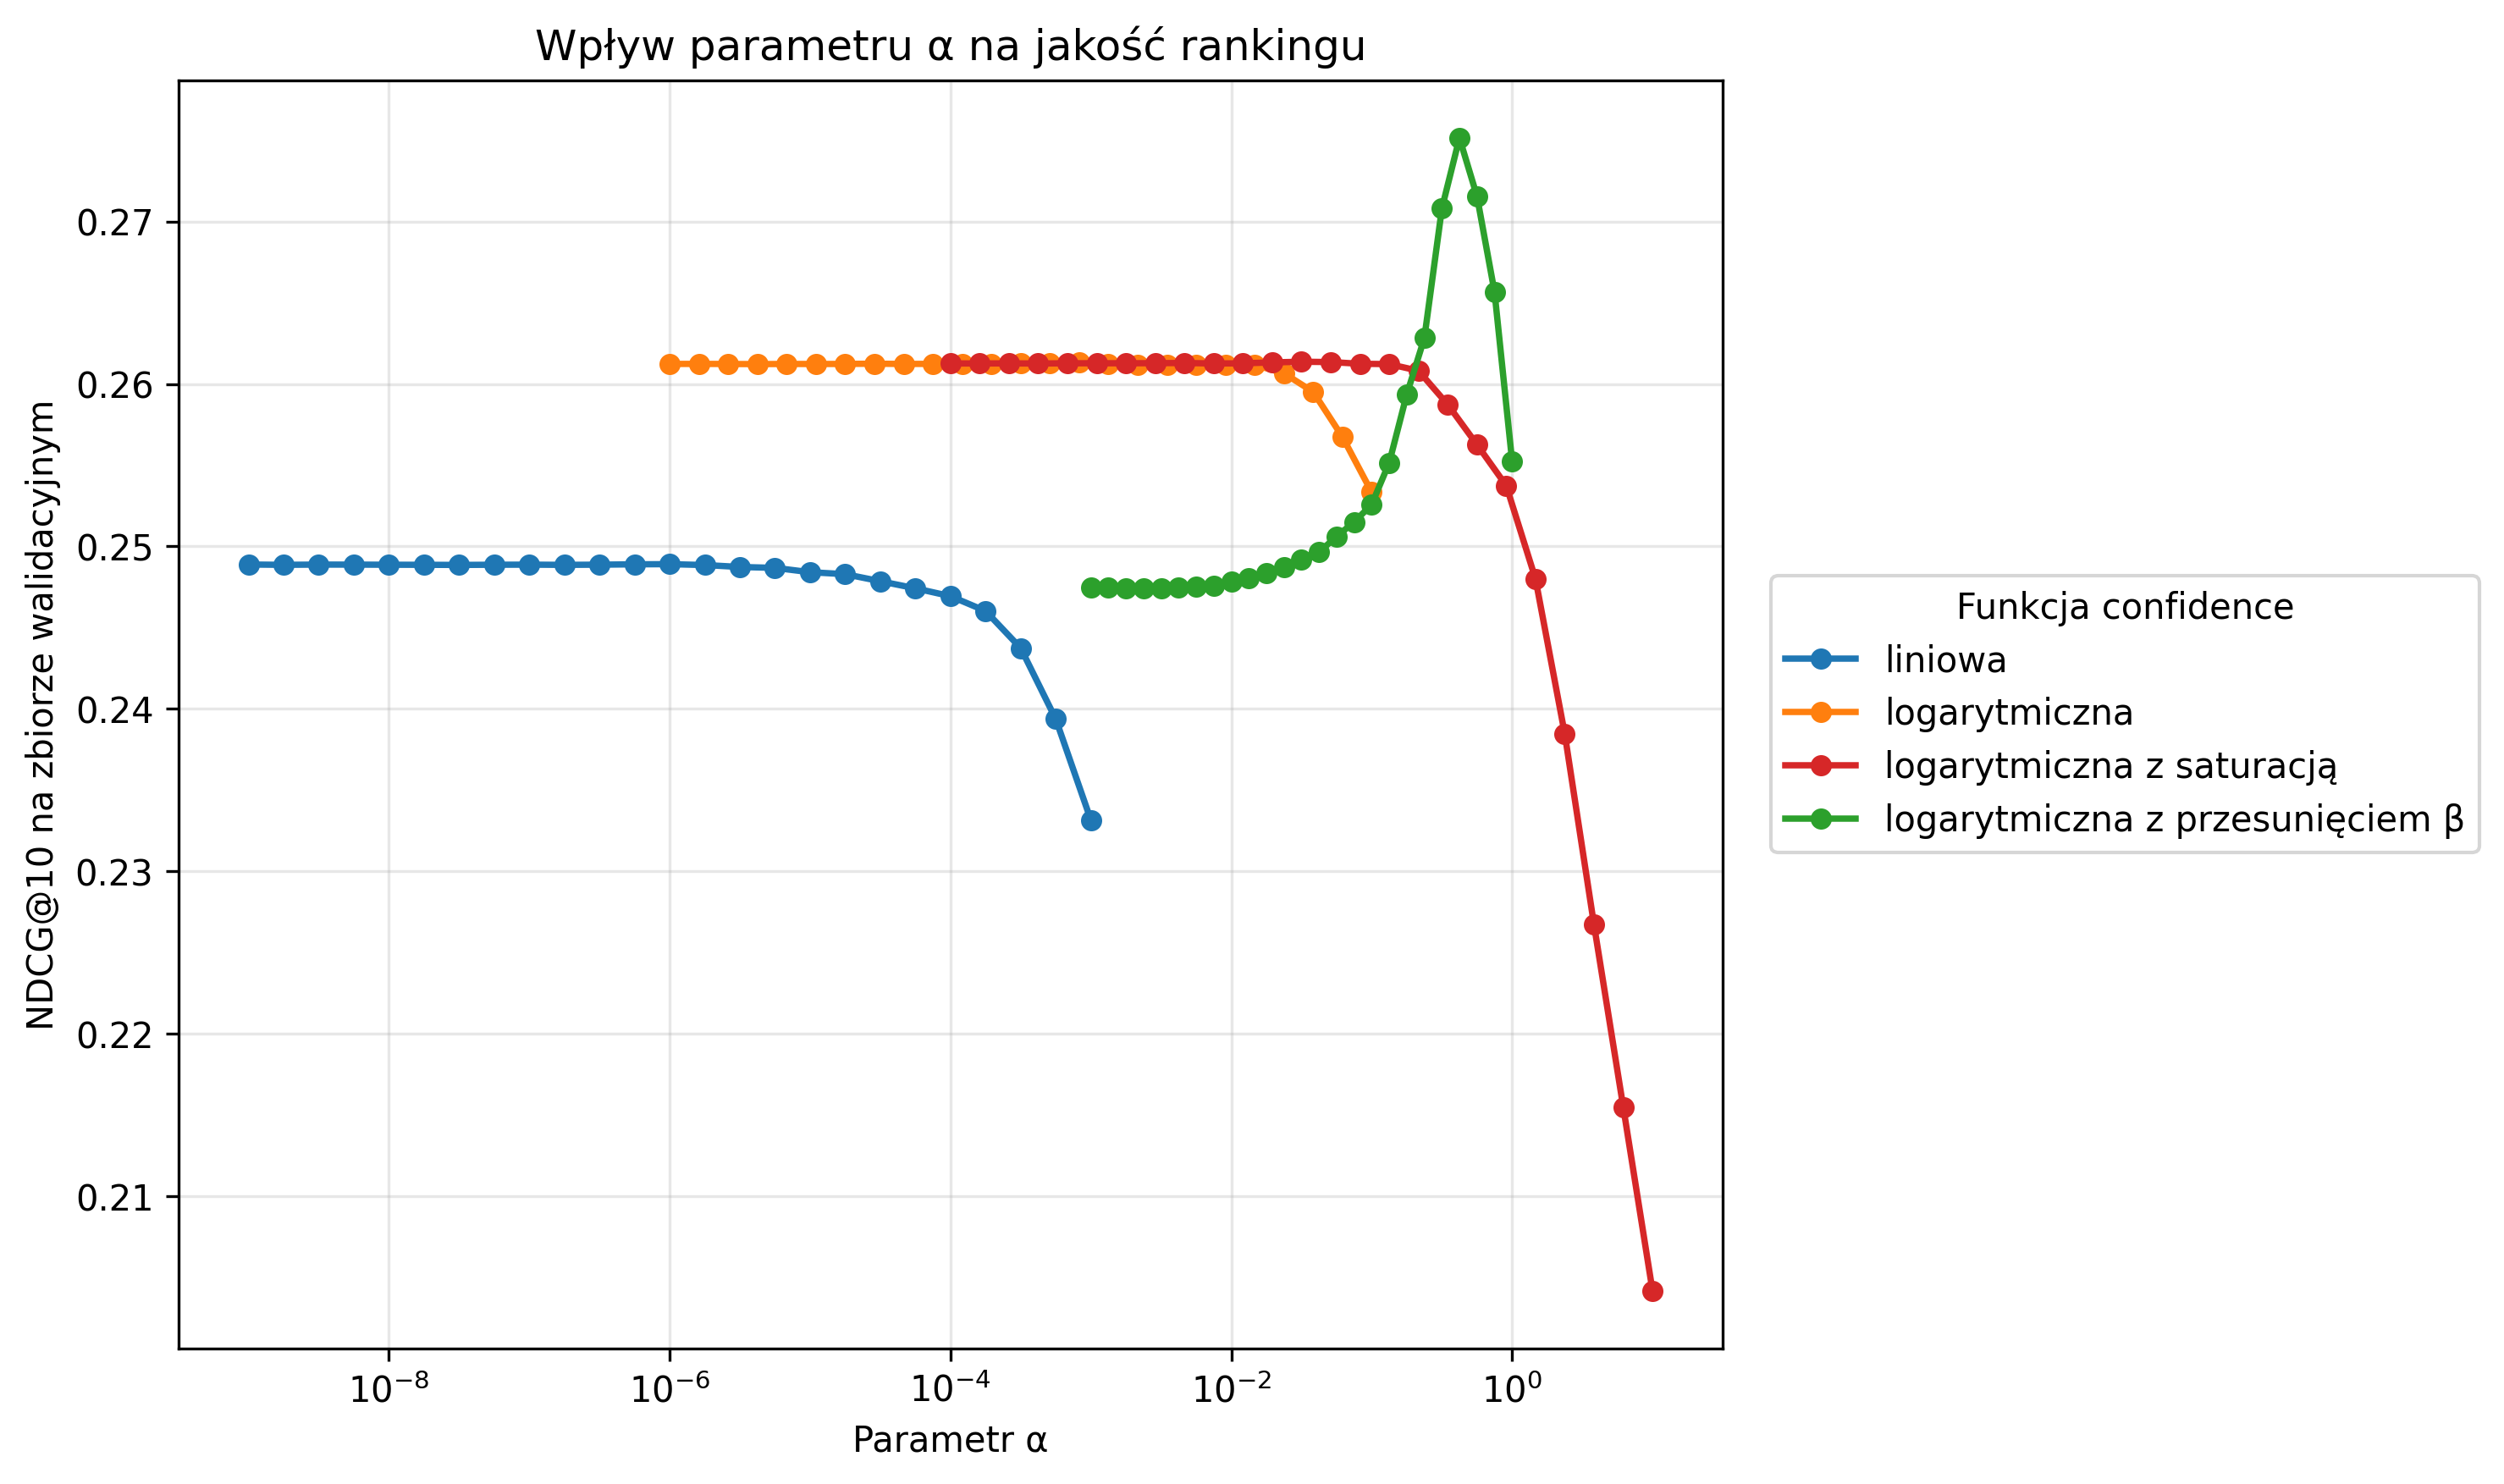
\includegraphics[width=0.9\textwidth]{../results/figures/wrazliwosc_ndcg_vs_alpha.png}
    \caption{Wrażliwość modeli na hiperparametr $\alpha$}
    \label{fig:wrazliwosc_ndcg_vs_alpha}
\end{figure}

Na wykresie~\ref{fig:wrazliwosc_ndcg_vs_alpha} widać, że dla każdej funkcji pewności z wyjątkiem logarytmicznej z przesunięciem $\beta$ wartości \ndcg{} są najwyższe dla $\alpha \rightarrow 0$, co odpowiada zredukowaniu sygnału zawartego w zmiennej \texttt{playtime\_forever} do postaci binarnej, odpowiadającej posiadaniu bądź nieposiadaniu danej gry. W celu zweryfikowania tej obserwacji w kolejnym podrozdziale zostały przebadane funkcje pewności zastosowane w modelach o optymalnych hiperparametrach. Jedynie dla wariantu z dodatkowym przesunięciem $\beta$ znalezione optimum $\alpha$ nie leży w otoczeniu zera. Nie oznacza to jednak, że wariant ten wykorzystuje informację o długości interakcji. Przy $\beta$ równym 108,284 przekształcenie działa w obszarze o niewielkiej krzywiźnie, a wyższa wartość $\alpha$ podnosi przede wszystkim ogólny poziom pewności, nie zaś stopień różnicowania obserwacji. Interpretację tę potwierdza wariant o stałej funkcji pewności, w którym różnicowanie zostało wyeliminowane całkowicie, a mimo to uzyskano najwyższą wartość \ndcg{}.

\begin{figure}[htbp]
    \centering
    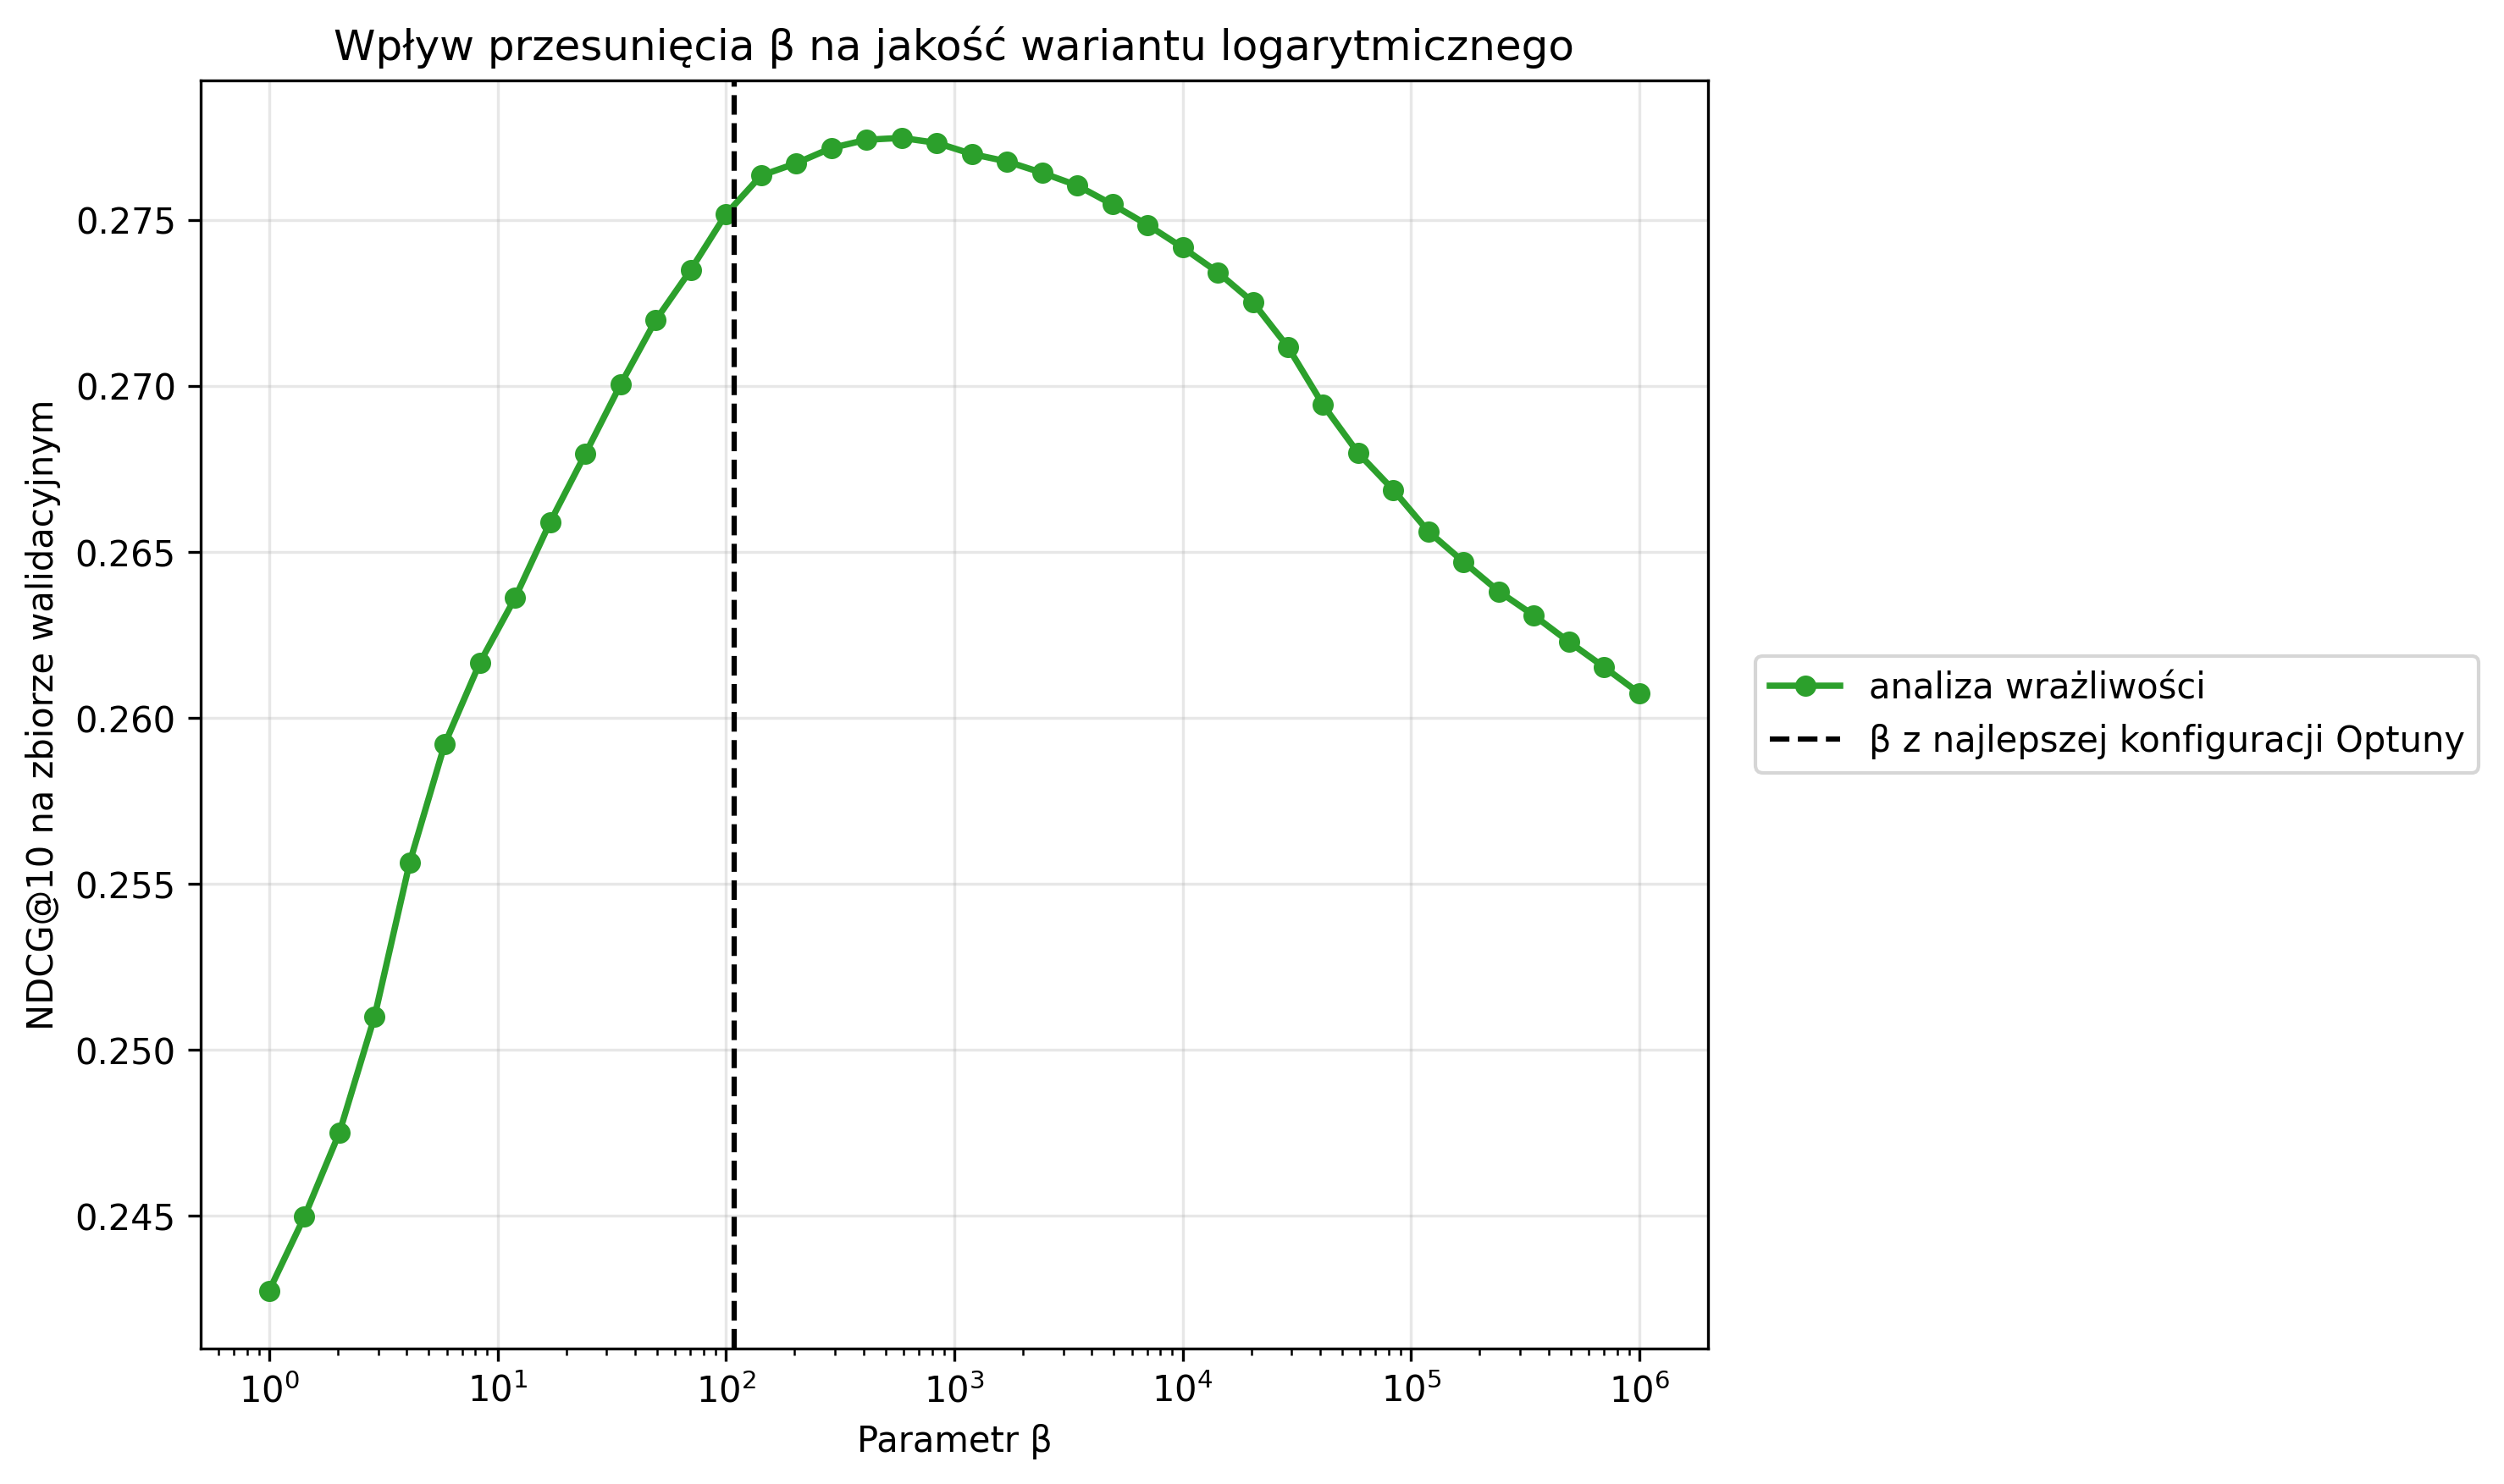
\includegraphics[width=0.9\textwidth]{../results/figures/wrazliwosc_log_beta_ndcg_vs_beta.png}
    \caption{Wrażliwość modelu na hiperparametr $\beta$}
    \label{fig:wrazliwosc_log_beta_ndcg_vs_beta}
\end{figure}

Analogiczną zależność od parametru $\beta$ przedstawiono na wykresie~\ref{fig:wrazliwosc_log_beta_ndcg_vs_beta}. Widać na nim, że wraz ze wzrostem hiperparametru \ndcg{} rośnie, osiągając maksimum dla wartości z rzędu od $10^2$ do $10^4$. Warto podkreślić, że $\beta$ zwiększa wartość $c_{ui}$ obserwacji z \texttt{playtime\_forever} = 0, która w pozostałych modelach zawsze wynosi 1. Dla $\beta$ z otoczenia maksimum mediana wartości pewności rośnie od 1{,}86 przy $\beta$ równym 100 do 3{,}50 przy $\beta$ równym 1000, obejmując tym samym poziom 3{,}364 uzyskany w wariancie o stałej funkcji pewności. Dodatkowo proces strojenia obu modeli doprowadził je do tej samej liczby czynników ukrytych. Warianty różnią się siłą regularyzacji, przy czym obie wartości pozostają w tym samym rzędzie wielkości. Dalsze zwiększanie $\beta$ prowadzi do stopniowego pogorszenia jakości rekomendacji. Wraz z jego wzrostem przekształcenie logarytmiczne dąży do stałej postaci, a średni poziom pewności rośnie. Przez wspólne występowanie obu efektów oraz wpływ regularyzacji na podstawie wyłącznie tego eksperymentu niemożliwe jest stwierdzenie, co dokładnie powoduje spadek jakości. Na wykresie można również zauważyć, że hiperparametry wybrane w procesie strojenia nie są w pełni optymalne, jednak ze względu na marginalność różnic eksperyment był kontynuowany bez ich zmiany.
\begin{figure}[htbp]
    \centering
    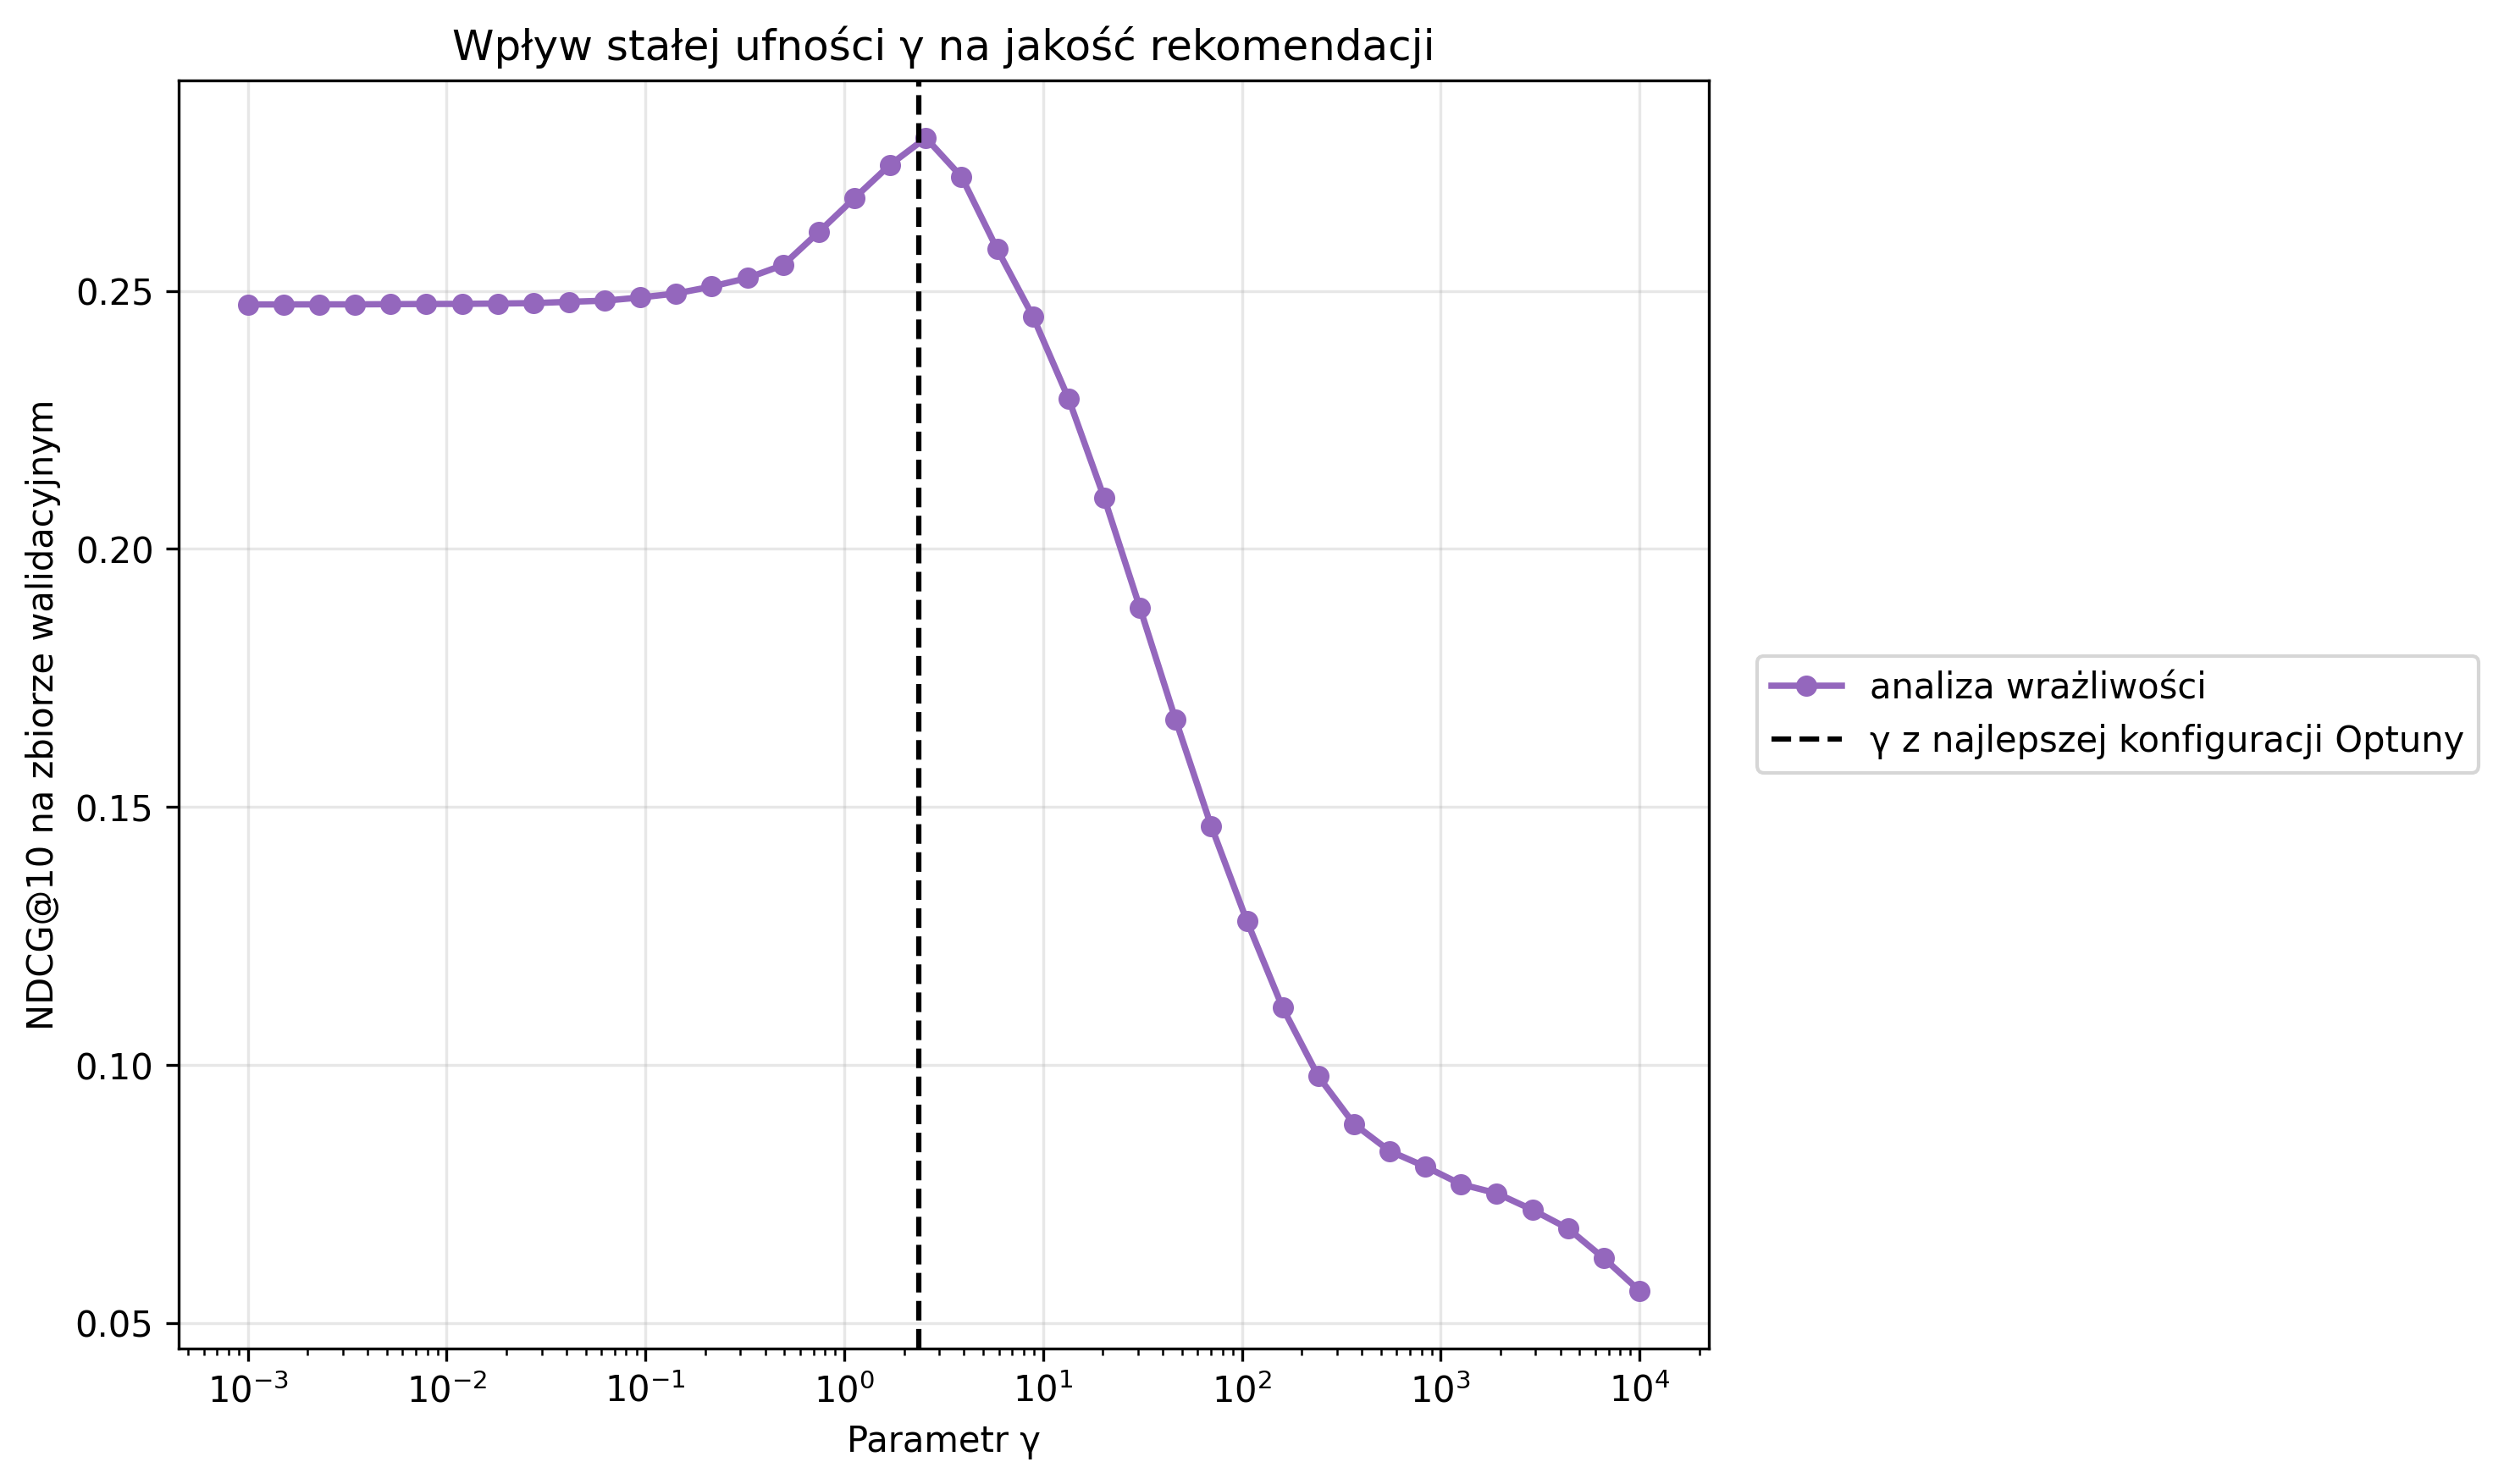
\includegraphics[width=0.9\textwidth]{../results/figures_revised/wrazliwosc_constant_ndcg_vs_gamma.png}
    \caption{Wrażliwość modelu na hiperparametr $\gamma$}
    \label{fig:wrazliwosc_ndcg_vs_gamma}
\end{figure}

Wykres~\ref{fig:wrazliwosc_ndcg_vs_gamma} przedstawia wrażliwość wariantu o stałej funkcji pewności na parametr $\gamma$, wyznaczającego globalny poziom pewności przy całkowitym pominięciu czasu gry. Krzywa ma wyraźne maksimum w okolicy $\gamma$ równego 2{,}5 i opada po obu stronach optimum. Dla $\gamma$ zbliżającego się do zera wartość $c_{ui}$ dąży do jedności, a zatem model traktuje brak interakcji jako równie istotny sygnał jak jej zaobserwowanie. Skutkuje to obniżeniem \ndcg{} do wartości 0{,}247. Dla wartości rzędu $10^4$ jakość rekomendacji drastycznie spada do 0{,}056, ponieważ nadmierna pewność prowadzi do przeuczenia modelu na zaobserwowanych interakcjach. Wynik ten pokazuje, że sam poziom pewności przypisany zaobserwowanym interakcjom istotnie wpływa na jakość rekomendacji, nawet gdy wagi nie różnicują obserwacji w żaden sposób.

Wartości hiperparametrów otrzymane w procesie strojenia modelu BPR zostały przedstawione w tabeli~\ref{tab:hiperparametry-bpr}.

\begin{table}[htbp]
\centering
\caption{Najlepsze hiperparametry modelu BPR wybrane na zbiorze walidacyjnym}
\label{tab:hiperparametry-bpr}
\begin{tabular}{lrrrrr}
\toprule
Wariant & $f$ & $\eta$ & $\lambda_\Theta$ & Iteracje & \ndcg{} \\
\midrule
BPR & $96$ & $0{,}001760$ & $0{,}003237$ & $150$ & $0{,}212$ \\
\bottomrule
\end{tabular}
\caption*{\footnotesize Źródło: opracowanie własne na podstawie wyników optymalizacji hiperparametrów.}
\end{table}


W przypadku modelu BPR nie jest możliwa tak dogłębna analiza dobranych hiperparametrów, ze względu na to, że interakcje traktowane są w sposób binarny. Długość kroku uczenia wpływa wyłącznie na proces wyznaczania maksimum prawdopodobieństwa a posteriori cech ukrytych. Natomiast wymiar przestrzeni cech ukrytych wraz z siłą regularyzacji pozwalają jedynie na oszacowanie złożoności odwzorowywanych relacji oraz swobody, jaką model dysponuje przy tworzeniu wektorów latentnych. Wybrana konfiguracja, obejmująca wyższą liczbę czynników niż w którymkolwiek z wariantów implicit ALS przy stosunkowo niewielkiej regularyzacji, sugeruje lepszą zdolność do tworzenia różnorodnych rekomendacji. Ta kwestia zostanie jednak poddana dalszej analizie w podrozdziale~\ref{sec:compromises_analysis}. 

\section{Analiza funkcji pewności}
\label{sec:confidence_analysis}

Aby zweryfikować hipotezę o redukcji sygnału z \texttt{playtime\_forever} w przypadku modeli implicit ALS przeprowadzono dodatkową analizę funkcji pewności otrzymanych w modelach. Na wykresie~\ref{fig:confidence_levels_best_als} przedstawiono ich zakres wartości dla każdego z modeli.

\begin{figure}[htbp]
    \centering
    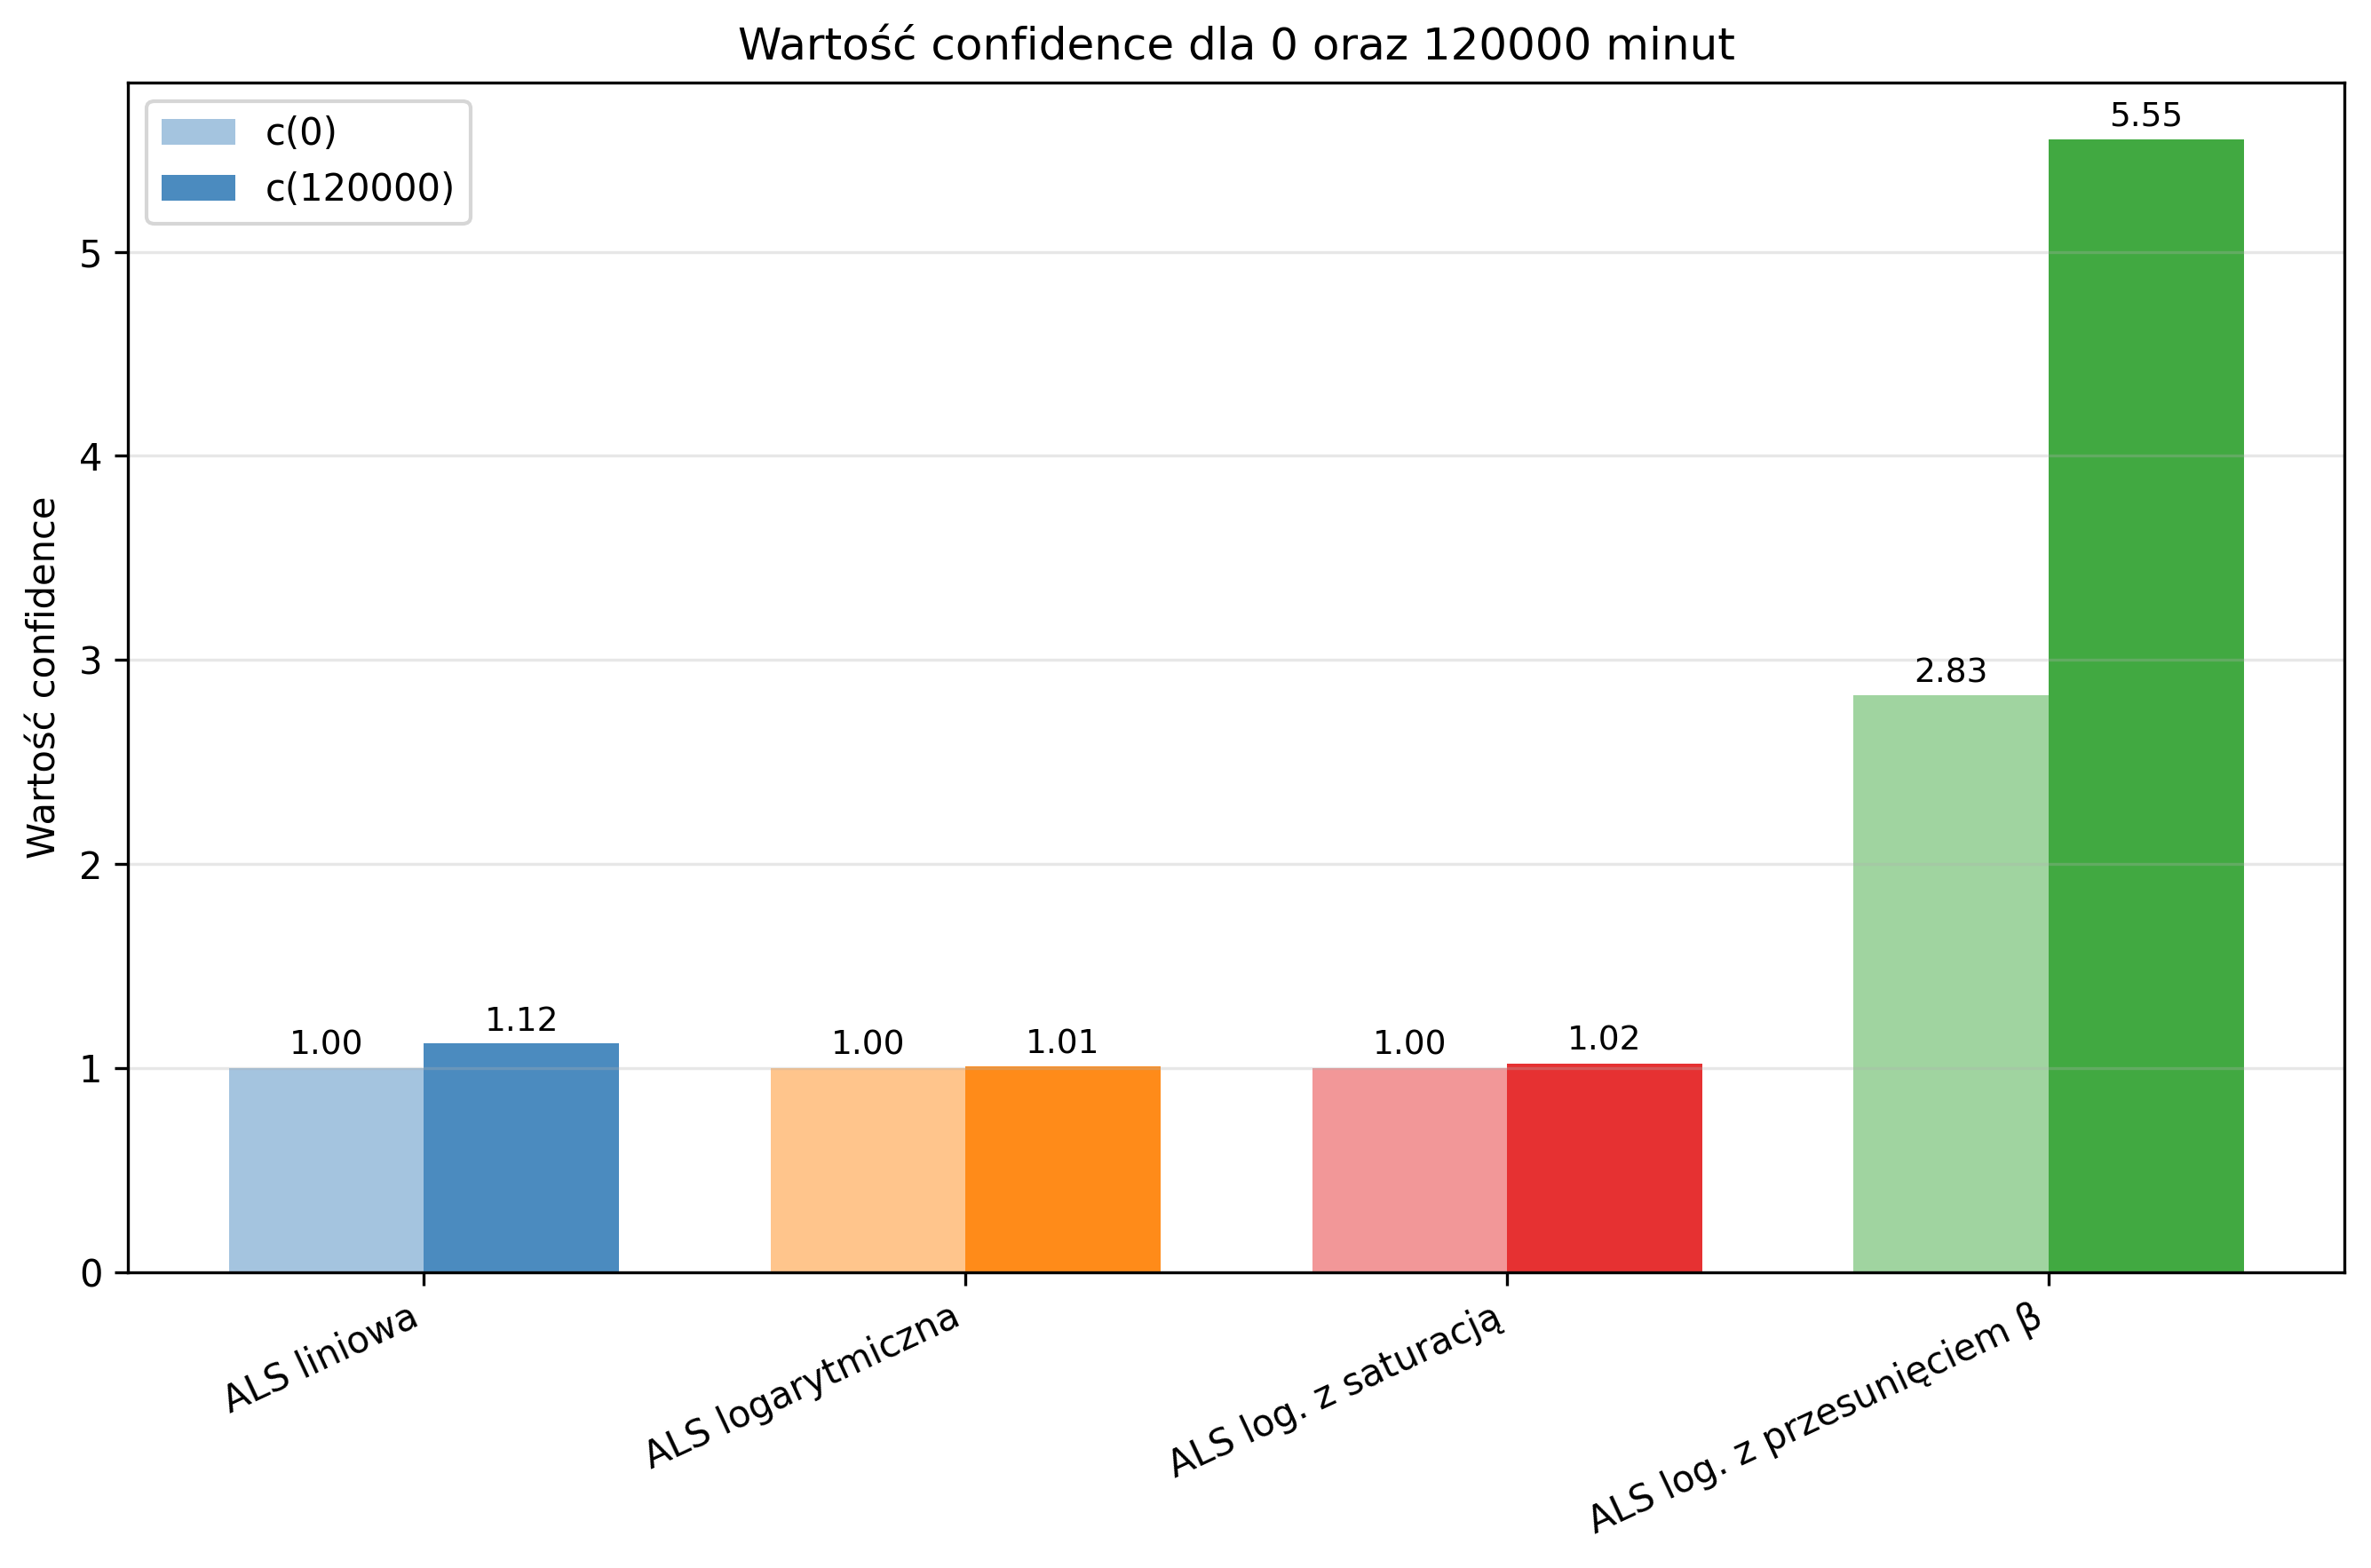
\includegraphics[width=0.9\textwidth]{../results/figures/confidence_levels_best_als.png}
    \caption{Zakres przyjmowanych wartości funkcji pewności}
    \label{fig:confidence_levels_best_als}
\end{figure}

W przypadku modelu z logarytmem oraz logarytmem z saturacją wykres~\ref{fig:confidence_levels_best_als} potwierdza, że długości interakcji mają bardzo znikomy wpływ na proces uczenia. Podobnie w przypadku modelu z liniową funkcją pewności zakresy wartości są niewielkie. Jedynie model z logarytmicznym przekształceniem z przesunięciem $\beta$ po wytrenowaniu uzyskał zakres pewności, który najdłuższym interakcjom przypisuje dwukrotnie większą wartość niż tym bez zarejestrowanego czasu gry.

Zestawienie tego zakresu z wariantem stałym prowadzi jednak do nieoczekiwanego wniosku. Przesunięcie $\beta$ podnosi dolną granicę zakresu funkcji odpowiadającą obserwacjom z zerowym czasem gry z wartości równej 1 do poziomu 2,83. Dla mediany czasu gry wynoszącej 35 minut wartość ta rośnie zaledwie do 2,94, pozostając w tym samym rzędzie co stała wartość 3,364 dobrana w wariancie pomijającym czas gry. Zatem dla znacznej części zbioru przekształcenie działa w wąskim przedziale wokół poziomu, który sam w sobie okazuje się wystarczający do uzyskania lepszych rekomendacji, a zróżnicowanie wag ujawnia się dopiero dla obserwacji z długiego ogona rozkładu.

Należy jednak podkreślić, że w procesie optymalizacji modelu implicit ALS uwzględniane są wszystkie możliwe kombinacje par użytkownik--gra, a przy gęstości macierzy interakcji wynoszącej 0,00887 przypadki niezaobserwowane, dla których $c_{ui} = 1$, zdecydowanie dominują w funkcji celu. Zmiana wartości $c_{ui}$ dla nielicznych interakcji pozytywnych oddziałuje więc przede wszystkim przez ogólne podniesienie ich wagi względem tła, w mniejszym stopniu zaś przez wzajemne różnicowanie tych obserwacji. Wskazuje to, że przewaga wariantu z przesunięciem $\beta$ nad pozostałymi przekształceniami wynikała nie tyle z lepszego odwzorowania siły preferencji, ile z podniesienia pewności wszystkich zaobserwowanych interakcji, w tym tych z zerowym czasem gry. Wariant o stałej funkcji pewności realizuje ten sam mechanizm, bez przekształcenia czasu gry osiągając podobne rezultaty.

Aby przyjrzeć się bliżej kształtowi poszczególnych przekształceń, stworzono wykres~\ref{fig:confidence_growth_best_als_0_2400} przedstawiający przyrost wartości funkcji pewności w modelach implicit ALS w zależności od zmiennej \texttt{playtime\_forever} dla pierwszych 20 godzin rozgrywki.

\begin{figure}[htbp]
    \centering
    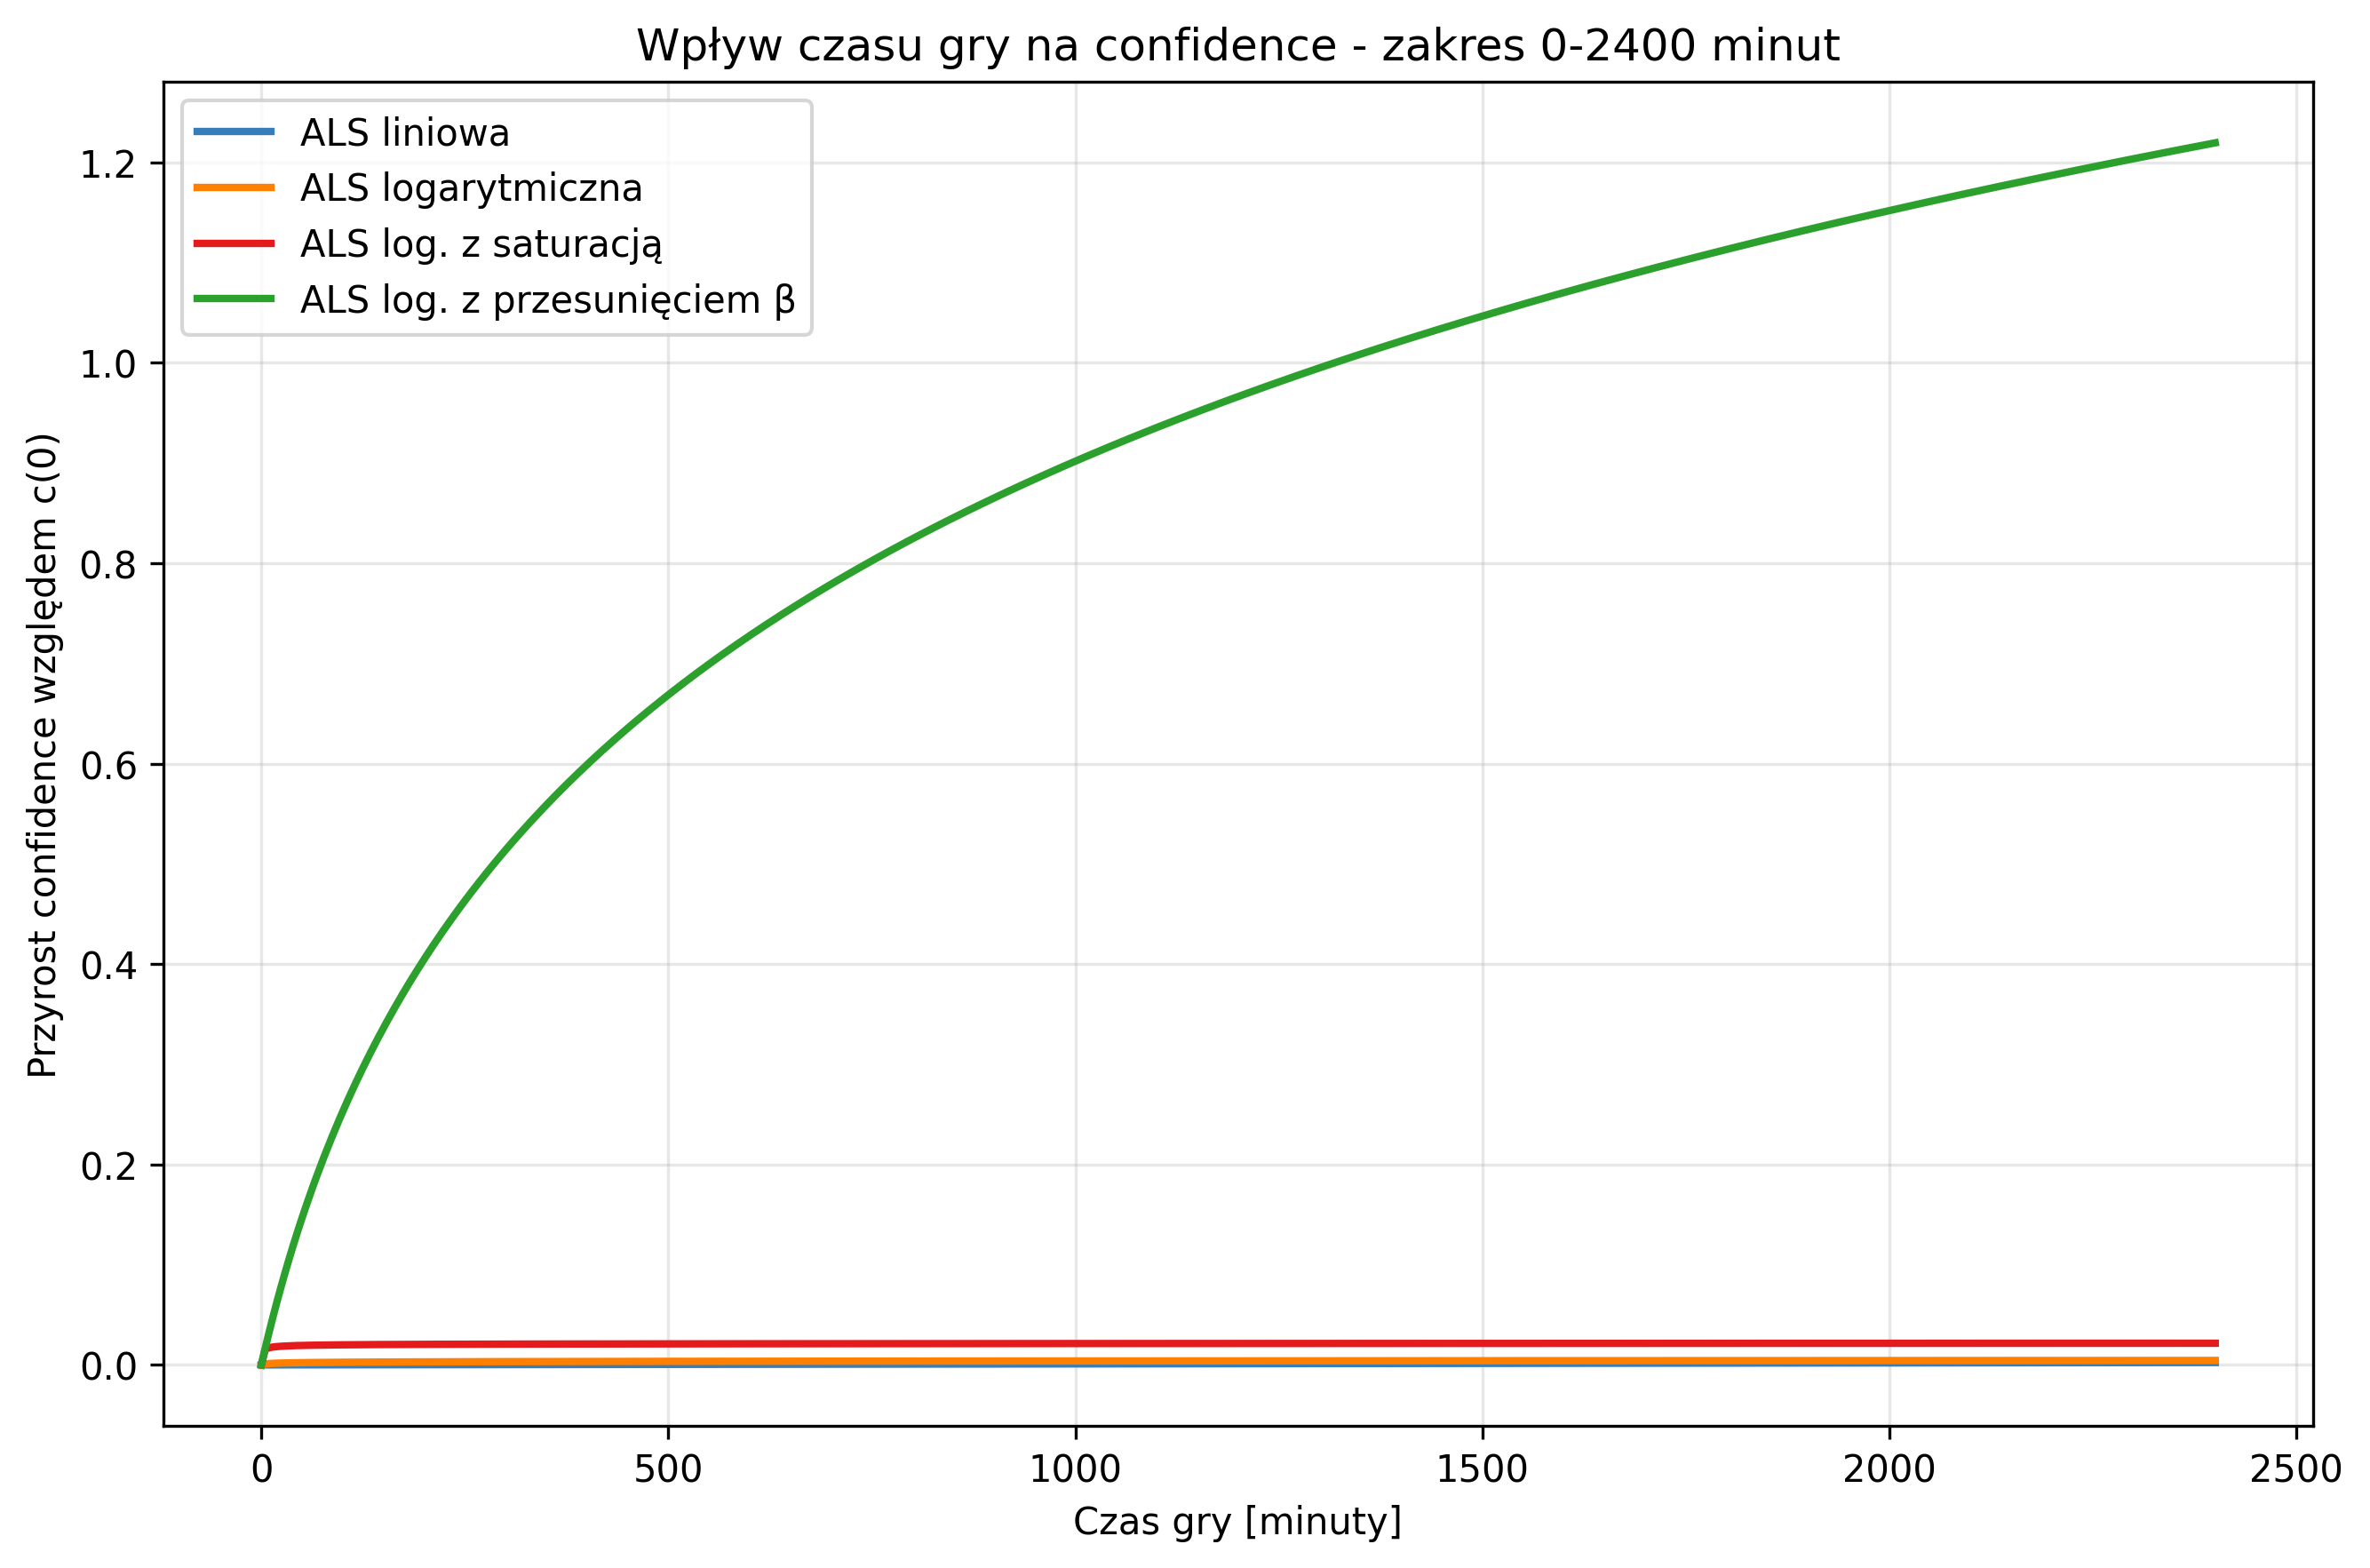
\includegraphics[width=0.9\textwidth]{../results/figures/confidence_growth_best_als_0_2400.png}
    \caption{Wartości pewności w zależności od zmiennej \texttt{playtime\_forever}}
    \label{fig:confidence_growth_best_als_0_2400}
\end{figure}

% ten wykres moze powinien byc nie przyrostem a po prostu wartoscią
% może też powinien być na całej skali od 0 do 120000

Przebieg krzywych na wykresie~\ref{fig:confidence_growth_best_als_0_2400} obrazuje różnicę między wariantem z przesunięciem $\beta$ a pozostałymi przekształceniami. Podczas gdy dla pozostałych modeli funkcja przyrostu wartości pewności pozostaje bliska 0, model z $c_{ui} = 1 + \alpha\log(1 + r_{ui} + \beta)$ wykazuje wyraźny wzrost. W przedziale pierwszych kilkuset minut rozgrywki przyrost wartości $c_{ui}$ jest stosunkowo szybki, natomiast w dalszej części wykresu krzywa widocznie łagodnieje. Należy jednak zestawić skalę tego przyrostu z poziomem bazowym. Dla mediany czasu gry przyrost względem $c(0)$ wynosi zaledwie 0,11 przy wartości bazowej 2,83. Widoczna na wykresie zmienność dotyczy zatem przede wszystkim mniejszościowej części zbioru, a dla typowego użytkownika funkcja pozostaje w wąskim otoczeniu wartości stałej.

Warto rozważyć teoretyczny przyrost pozostałych wariantów transformacji w przypadku, gdyby nie uległy one skrajnemu spłaszczeniu. Dla modelu z $c_{ui} = 1 + \alpha \log(r_{ui} + 1)$ dla domyślnego hiperparametru $\alpha = 1$ zaledwie 19 minut rozgrywki wystarczy, aby wartość pewności modelu gwałtownie skoczyła od poziomu bazowego równego 1 aż do 4. Równocześnie, aby uzyskać wzrost z poziomu 7 do 8, użytkownik musi spędzić w grze w przybliżeniu dodatkowe 11 i pół godziny. Oznacza to, że ta funkcja wykazuje się znaczną czułością w wąskim przedziale małych wartości, podczas gdy zmiana wśród dużych wartości jest nieznaczna. Podobny efekt obserwuje się w przypadku funkcji
$c_{ui} = 1 + \alpha \frac{\log(1 + r_{ui})}{1 + \log(1 + r_{ui})}$. Natomiast w przypadku liniowej funkcji pewności $c_{ui} = 1 + \alpha r_{ui}$ to zjawisko przybiera odwrotny charakter. Ponieważ jej przyrost jest proporcjonalny do spędzonego czasu, model nie posiada efektu saturacji. W efekcie użytkownicy generujący skrajnie wysokie liczby godzin uzyskiwaliby dominujący wpływ na wartość funkcji straty. Proces optymalizacji hiperparametrów przeciwdziała temu, dobierając $\alpha$ rzędu $10^{-6}$, co w praktyce sprowadza przekształcenie do postaci niemal stałej. Zarówno w tym przypadku, jak i dla wariantów logarytmicznych, optymalizacja konsekwentnie zmierza zatem w stronę ograniczenia zróżnicowania wag, niezależnie od kształtu samego przekształcenia.

\section{Jakość rekomendacji na zbiorze testowym}

Przedstawione różnice w procesie uczenia mają swoje odzwierciedlenie w metrykach otrzymanych na zbiorze testowym. W tabeli~\ref{tab:wyniki-glowne} przedstawiono uśrednione wyniki otrzymane dla każdego z modeli. Dla zachowania czytelności w~tabeli pominięto odchylenia standardowe;
przedstawiono je w~podrozdziale~\ref{sec:stabilnosc}.

\begin{table}[htbp]
\centering
\caption{Wyniki modeli na zbiorze testowym}
\label{tab:wyniki-glowne}
\resizebox{\textwidth}{!}{%
\begin{tabular}{lrrrrrr}
\toprule
Model & NDCG@10 & Precision@10 & Recall@10 & Coverage@10 & $\Delta$GAP@10 & ILD@10\\
\midrule
Popularność & $0{,}1855$ & $0{,}0965$ & $0{,}1783$ & $0{,}0087$ & $1{,}4233$ & --- \\
ALS liniowa & $0{,}3299$ & $0{,}1841$ & $0{,}2642$ & $0{,}1178$ & $-0{,}2112$ & $0{,}7528$ \\
ALS logarytmiczna & $0{,}3356$ & $0{,}1810$ & $0{,}3019$ & $0{,}0762$ & $0{,}5433$ & $0{,}6469$ \\
ALS log. z saturacją & $0{,}3354$ & $0{,}1809$ & $0{,}3019$ & $0{,}0761$ & $0{,}5443$ & $0{,}6470$ \\
ALS log. z przesunięciem $\beta$ & $0{,}3517$ & $0{,}1956$ & $0{,}3338$ & $0{,}1313$ & $0{,}4191$ & $0{,}6841$ \\
ALS stała & $\mathbf{0{,}3565}$ & $\mathbf{0{,}1978}$ & $\mathbf{0{,}3370}$ & $0{,}1374$ & $0{,}4210$ & $0{,}6825$ \\
BPR & $0{,}2703$ & $0{,}1329$ & $0{,}2614$ & $\mathbf{0{,}3039}$ & $-0{,}0789$ & $0{,}7363$ \\
\bottomrule
\end{tabular}%
}
\caption*{\footnotesize Źródło: opracowanie własne. Wartości dla ALS i BPR to średnie z~pięciu uruchomień, z~wyjątkiem ILD@10, wyznaczonej dla pojedynczego uruchomienia. Pogrubieniem oznaczono najlepszy wynik w~każdej kolumnie.}
\end{table}

Ze względu na dużą liczbę metryk w tym podrozdziale skupiono się na metrykach rankingowych, pozostałe z nich zostaną przeanalizowane w kolejnym podrozdziale poświęconym kompromisom między nimi. Ze względu na stosowanie metryki \ndcg{} jako głównej metryki rankingowej w celu lepszego zaprezentowania różnic między modelami utworzono wykres~\ref{fig:test_ndcg_all_models_horizontal}, który przedstawia jej wartość dla każdego z testowanych modeli.

\begin{figure}[htbp]
    \centering
    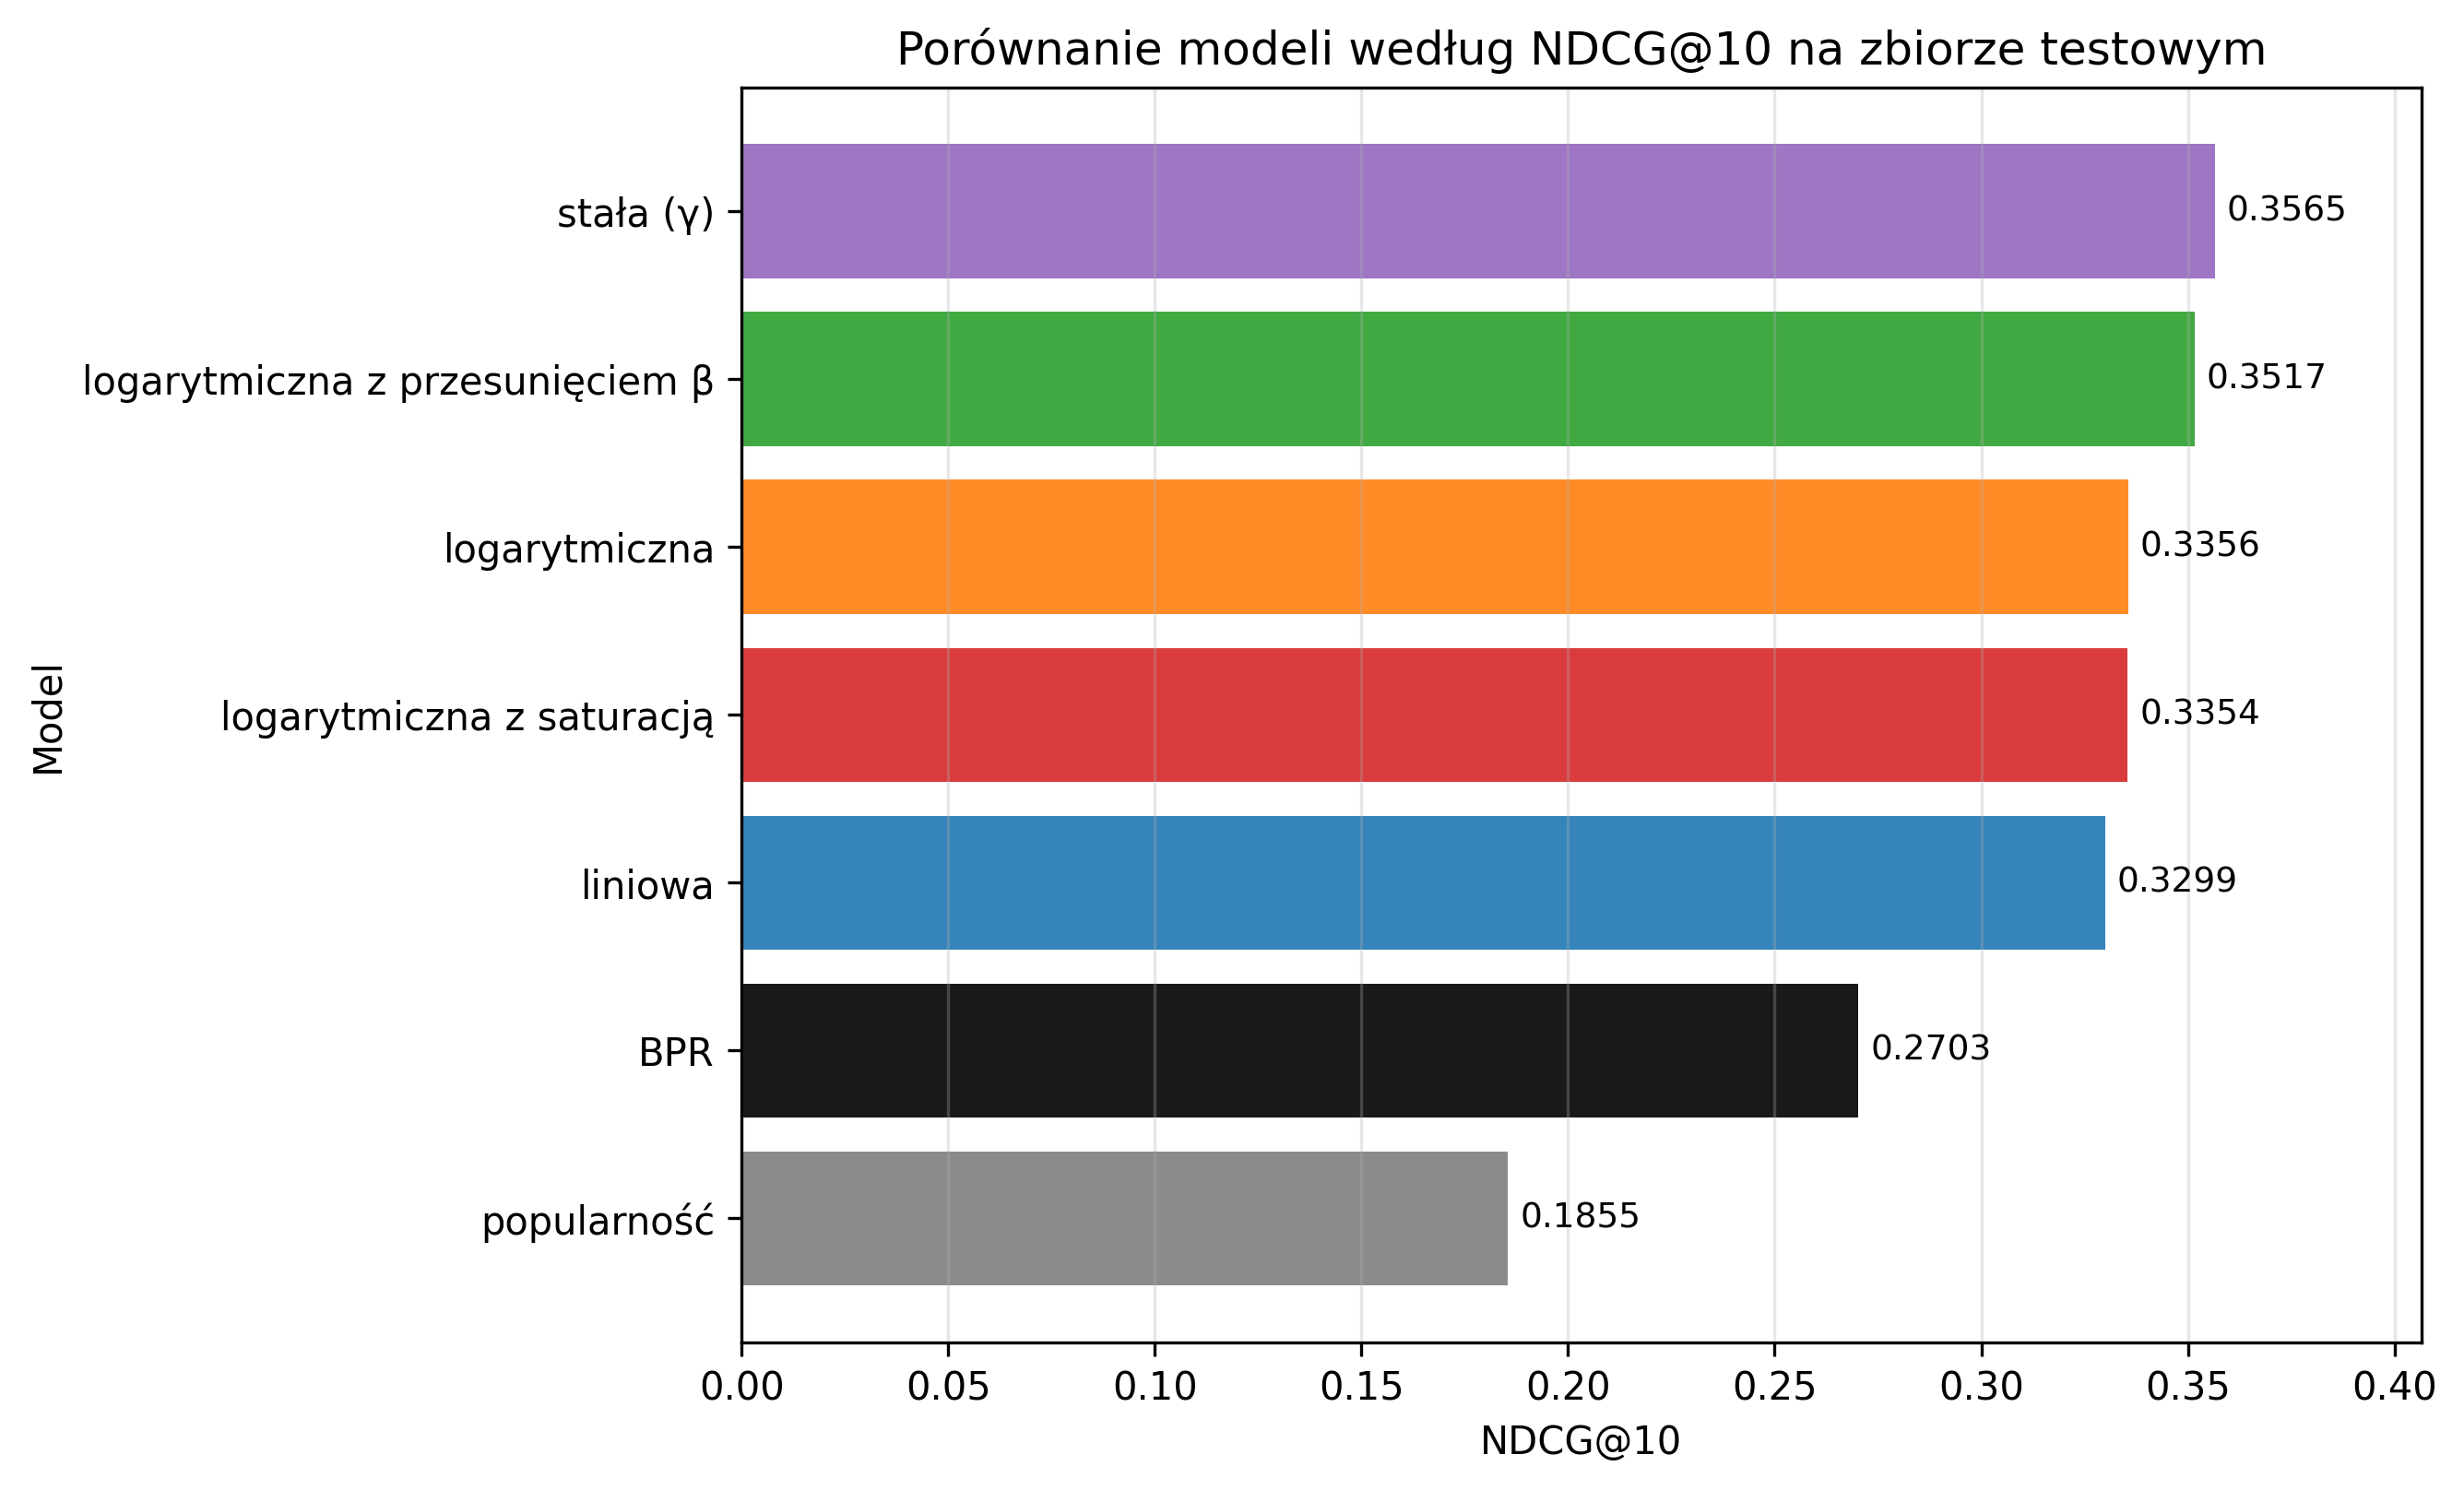
\includegraphics[width=0.9\textwidth]{../results/figures_revised/test_ndcg_all_models_horizontal.png}
    \caption{Wartości \ndcg{} każdego z modeli na zbiorze testowym}
    \label{fig:test_ndcg_all_models_horizontal}
\end{figure}

Wykres jednoznacznie pokazuje, że model popularnościowy cechuje się niższą zdolnością rekomendacji niż modele oparte na metodach faktoryzacji macierzy. Mimo to uzyskany wynik nie jest zaniedbywalny. Model popularnościowy efektywnie wykorzystuje silny efekt nierównomierności popularności gier w analizowanym zbiorze danych przedstawiony na wykresie~\ref{fig:filtered_item_popularity_concentration}. Ze względu na to został on wykorzystany jako punkt odniesienia w niniejszej pracy.

Uzyskana przez BPR wartość \ndcg{} jest najniższa spośród wszystkich modeli faktoryzacji. Należy jednak podkreślić, że nie oznacza to, że model jest obiektywnie gorszy. W ocenie systemów rekomendacyjnych należy również uwzględniać metryki odpowiedzialne za pokrycie katalogu i podatność na obciążenie popularnością.

Istotnych wniosków dostarcza porównanie poszczególnych wariantów modelu ALS między sobą. Najwyższą wartość \ndcg{} uzyskał model o stałej funkcji pewności (0,3565), co stanowi poprawę o 6,2\% względem wariantu logarytmicznego (0,3356) oraz o 8,1\% względem wariantu liniowego (0,3299). Drugi w kolejności wariant z przesunięciem $\beta$ (0,3517) ustępuje mu o 1,4\%. Uporządkowanie wariantów odpowiada zatem obserwacjom poczynionym na zbiorze walidacyjnym. Dwa najlepsze warianty łączy podniesienie pewności obserwacji o zerowym czasie gry, którym pozostałe przekształcenia przypisują wartość równą 1. Uzyskana poprawa względem bazowej implementacji ALS wskazuje, że wybór wariantu funkcji pewności wraz z~towarzyszącym mu doborem pozostałych hiperparametrów przekłada się na jakość rekomendacji przy zachowaniu tej
samej architektury modelu. Warto zauważyć, że podobne obserwacje zostały przedstawione w pracy~\cite{rendle2021revisiting}, gdzie autorzy pokazali, że odpowiednio dostrojone i zmodyfikowane warianty klasycznego implicit ALS mogą osiągać wyższe wyniki, a nawet konkurować z bardziej złożonymi modelami rekomendacyjnymi, w tym neuronowymi.

W celu potwierdzenia statystycznej istotności różnic przeprowadzono testy Wilcoxona dla par obserwacji na wartościach \ndcg{} wyznaczonych indywidualnie dla każdego użytkownika. Ze względu na dziesięć porównań parowych zastosowano korektę Holma-Bonferroniego. Wszystkie różnice okazały się istotne na poziomie istotności $0{,}05$, jednak należy podkreślić, że przy próbie liczącej 62\,944 użytkowników istotność osiągają również bardzo małe różnice, dlatego dodatkowo wyznaczono medianę i średnią sparowanej różnicy \ndcg{} wraz z 95-procentowym przedziałem ufności metodą bootstrapu po użytkownikach.

Mediana sparowanej różnicy \ndcg{} we wszystkich porównaniach wynosi zero, mimo że dla większości użytkowników porównywane warianty dają odmienne wyniki. W przypadku wariantu liniowego i stałego różnice odnotowano dla 83,9\% użytkowników. Wynika to z niemal symetrycznego rozkładu tych różnic wokół zera. Przewaga jednego z nich uwidacznia się dopiero w wartościach średnich, na które wpływa skala różnic w ogonach rozkładu. Oznacza to jednak, że dla pojedynczego użytkownika wybór zastosowanego modelu nie przekłada się na przewidywalną poprawę jakości rekomendacji. Żaden z wyznaczonych przedziałów ufności nie obejmuje zera, co potwierdza istotność statystyczną różnic między wariantami modelu iALS.

Najmniejszą różnicę zaobserwowano między wariantem logarytmicznym i logarytmicznym z saturacją, dla których wynosi ona zaledwie $-0{,}0002$ przy przedziale ufności $[-0{,}0003; -0{,}0001]$. Warianty te są zatem w praktyce nierozróżnialne, co jest spójne z wcześniejszymi obserwacjami dotyczącymi zbliżonego kształtu obu przekształceń. Największą różnicę odnotowano między wariantem stałym a~liniowym, dla których średnia sparowana różnica \ndcg{} wynosi 0{,}0266 przy przedziale ufności $[0{,}0248;\ 0{,}0284]$. Różnica między dwoma najlepszymi wariantami, stałym oraz z przesunięciem $\beta$, wynosi natomiast 0,0049 przy przedziale $[0{,}0045; 0{,}0052]$.

Dodatkowych informacji dostarcza odsetek użytkowników, dla których żadna z rekomendowanych pozycji nie okazała się trafiona. W wariancie liniowym zerową wartość \ndcg{} odnotowano dla 24,4\% użytkowników, w wariantach logarytmicznych dla 19,8\%, natomiast w wariancie stałym oraz z przesunięciem $\beta$ dla 14,8\%. Dwa najlepsze warianty generują więc co najmniej jedną trafioną rekomendację dla blisko sześciu tysięcy użytkowników więcej niż wariant liniowy. Sugeruje to, że uzyskana poprawa nie polega wyłącznie na lepszym uszeregowaniu pozycji dla użytkowników już obsługiwanych, ale również na zmniejszeniu liczby tych, dla których rekomendacje są całkowicie nietrafione.

W przypadku metryk precyzji i pełności ich rola jest ograniczona ze względu na ich silną korelację z \ndcg{} wynikające z faktu, że wszystkie te metryki oceniają trafność rekomendacji na podstawie liczby trafień elementów istotnych dla użytkownika. Jednak mogą one pokazać różnice w jakości rekomendacji w zależności od poziomu aktywności użytkownika.
 

\begin{figure}[htbp]
    \centering
    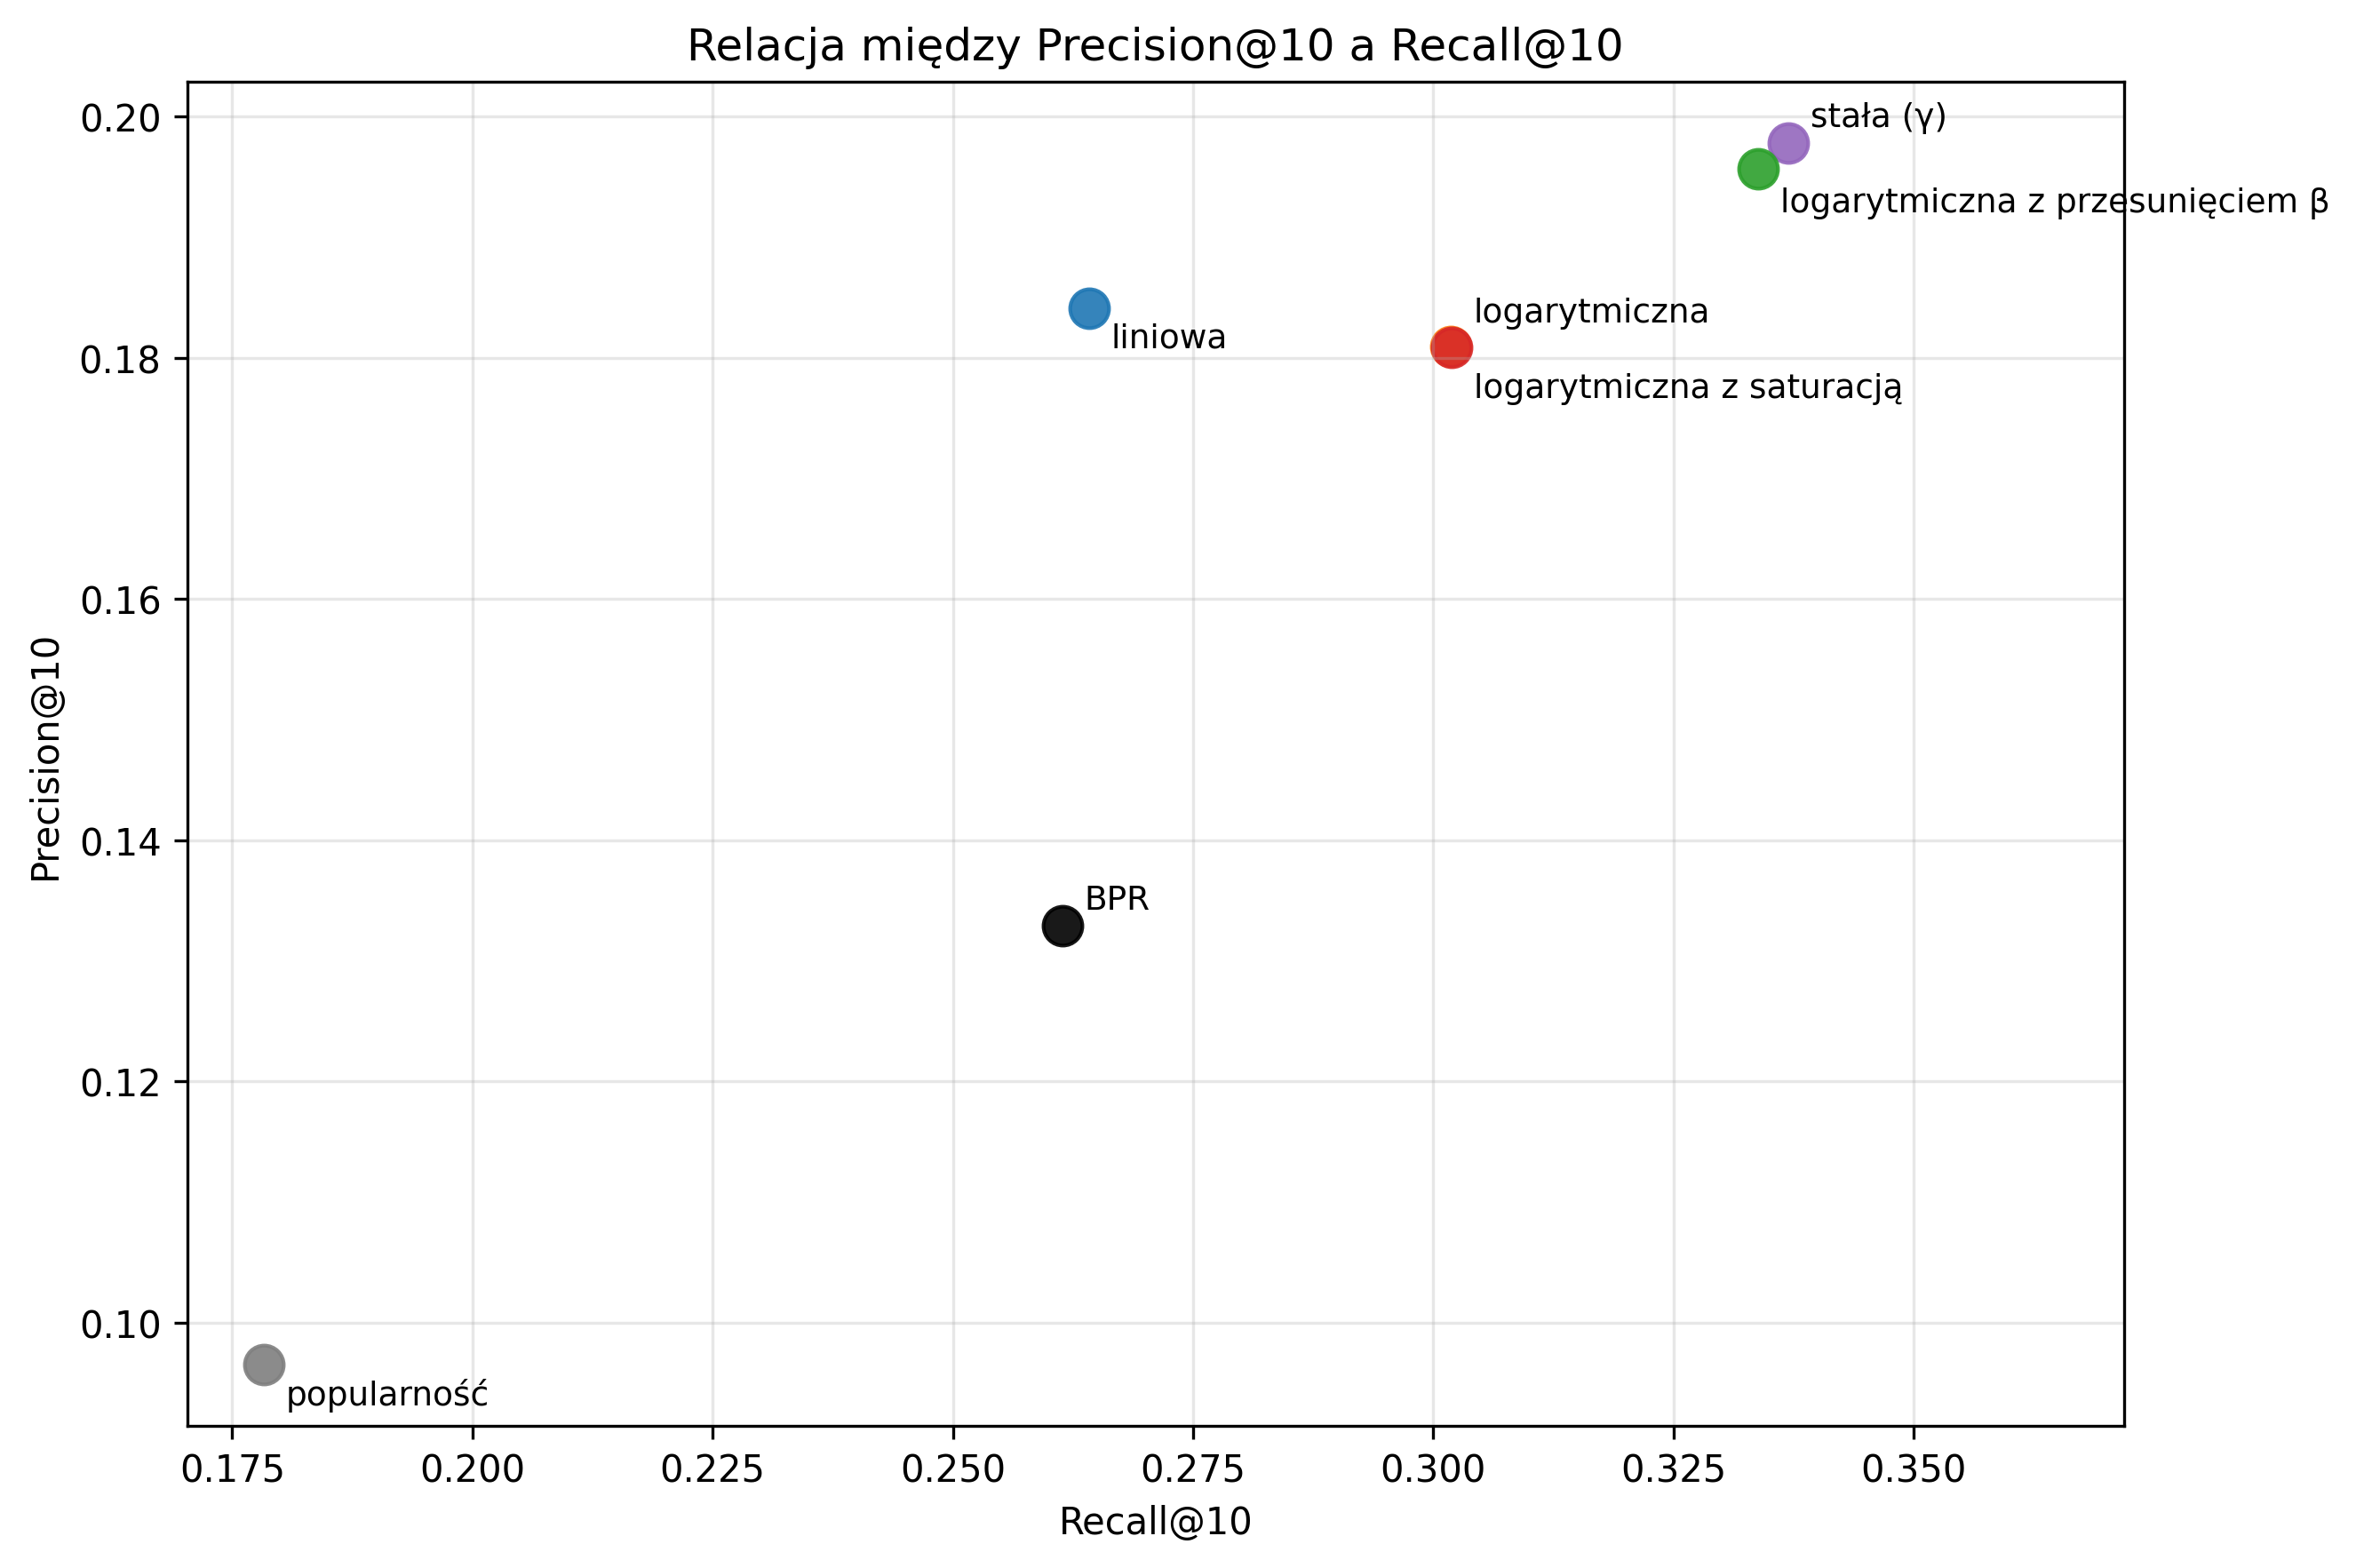
\includegraphics[width=0.9\textwidth]{../results/figures_revised/test_precision_vs_recall_all_models.png}
    \caption{Wartości precyzji względem pełności na zbiorze testowym}
    \label{fig:test_precision_vs_recall_all_models}
\end{figure}

Z wykresu~\ref{fig:test_precision_vs_recall_all_models} można zauważyć, że pomimo niższej wartości metryki pełności od modeli z przekształceniem logarytmicznym i logarytmicznym z saturacją model liniowy ma wyższą wartość precyzji. Może to sugerować, że ten model oferuje trafniejsze rekomendacje w przypadku użytkowników z większą liczbą interakcji. Weryfikacja tej hipotezy wymagałaby podziału użytkowników według liczby posiadanych interakcji, co wykracza poza zakres niniejszej pracy. Widoczne jest również, że warianty o stałej funkcji pewności oraz z przesunięciem $\beta$ wypadają najlepiej w kontekście obu analizowanych metryk, przy czym leżą na wykresie blisko siebie.

\section{Analiza kompromisów jakości rekomendacji}
\label{sec:compromises_analysis}

W procesie ewaluacji systemów rekomendacyjnych istotne jest uwzględnienie również metryk wykraczających poza trafność predykcji (ang. \textit{beyond-accuracy}), takich jak pokrycie katalogu, różnorodność oraz $\Delta$GAP. W niniejszym podrozdziale poddano analizie kompromisy między jakością rekomendacji a wspomnianymi wyżej miarami.

\begin{figure}[htbp]
    \centering
    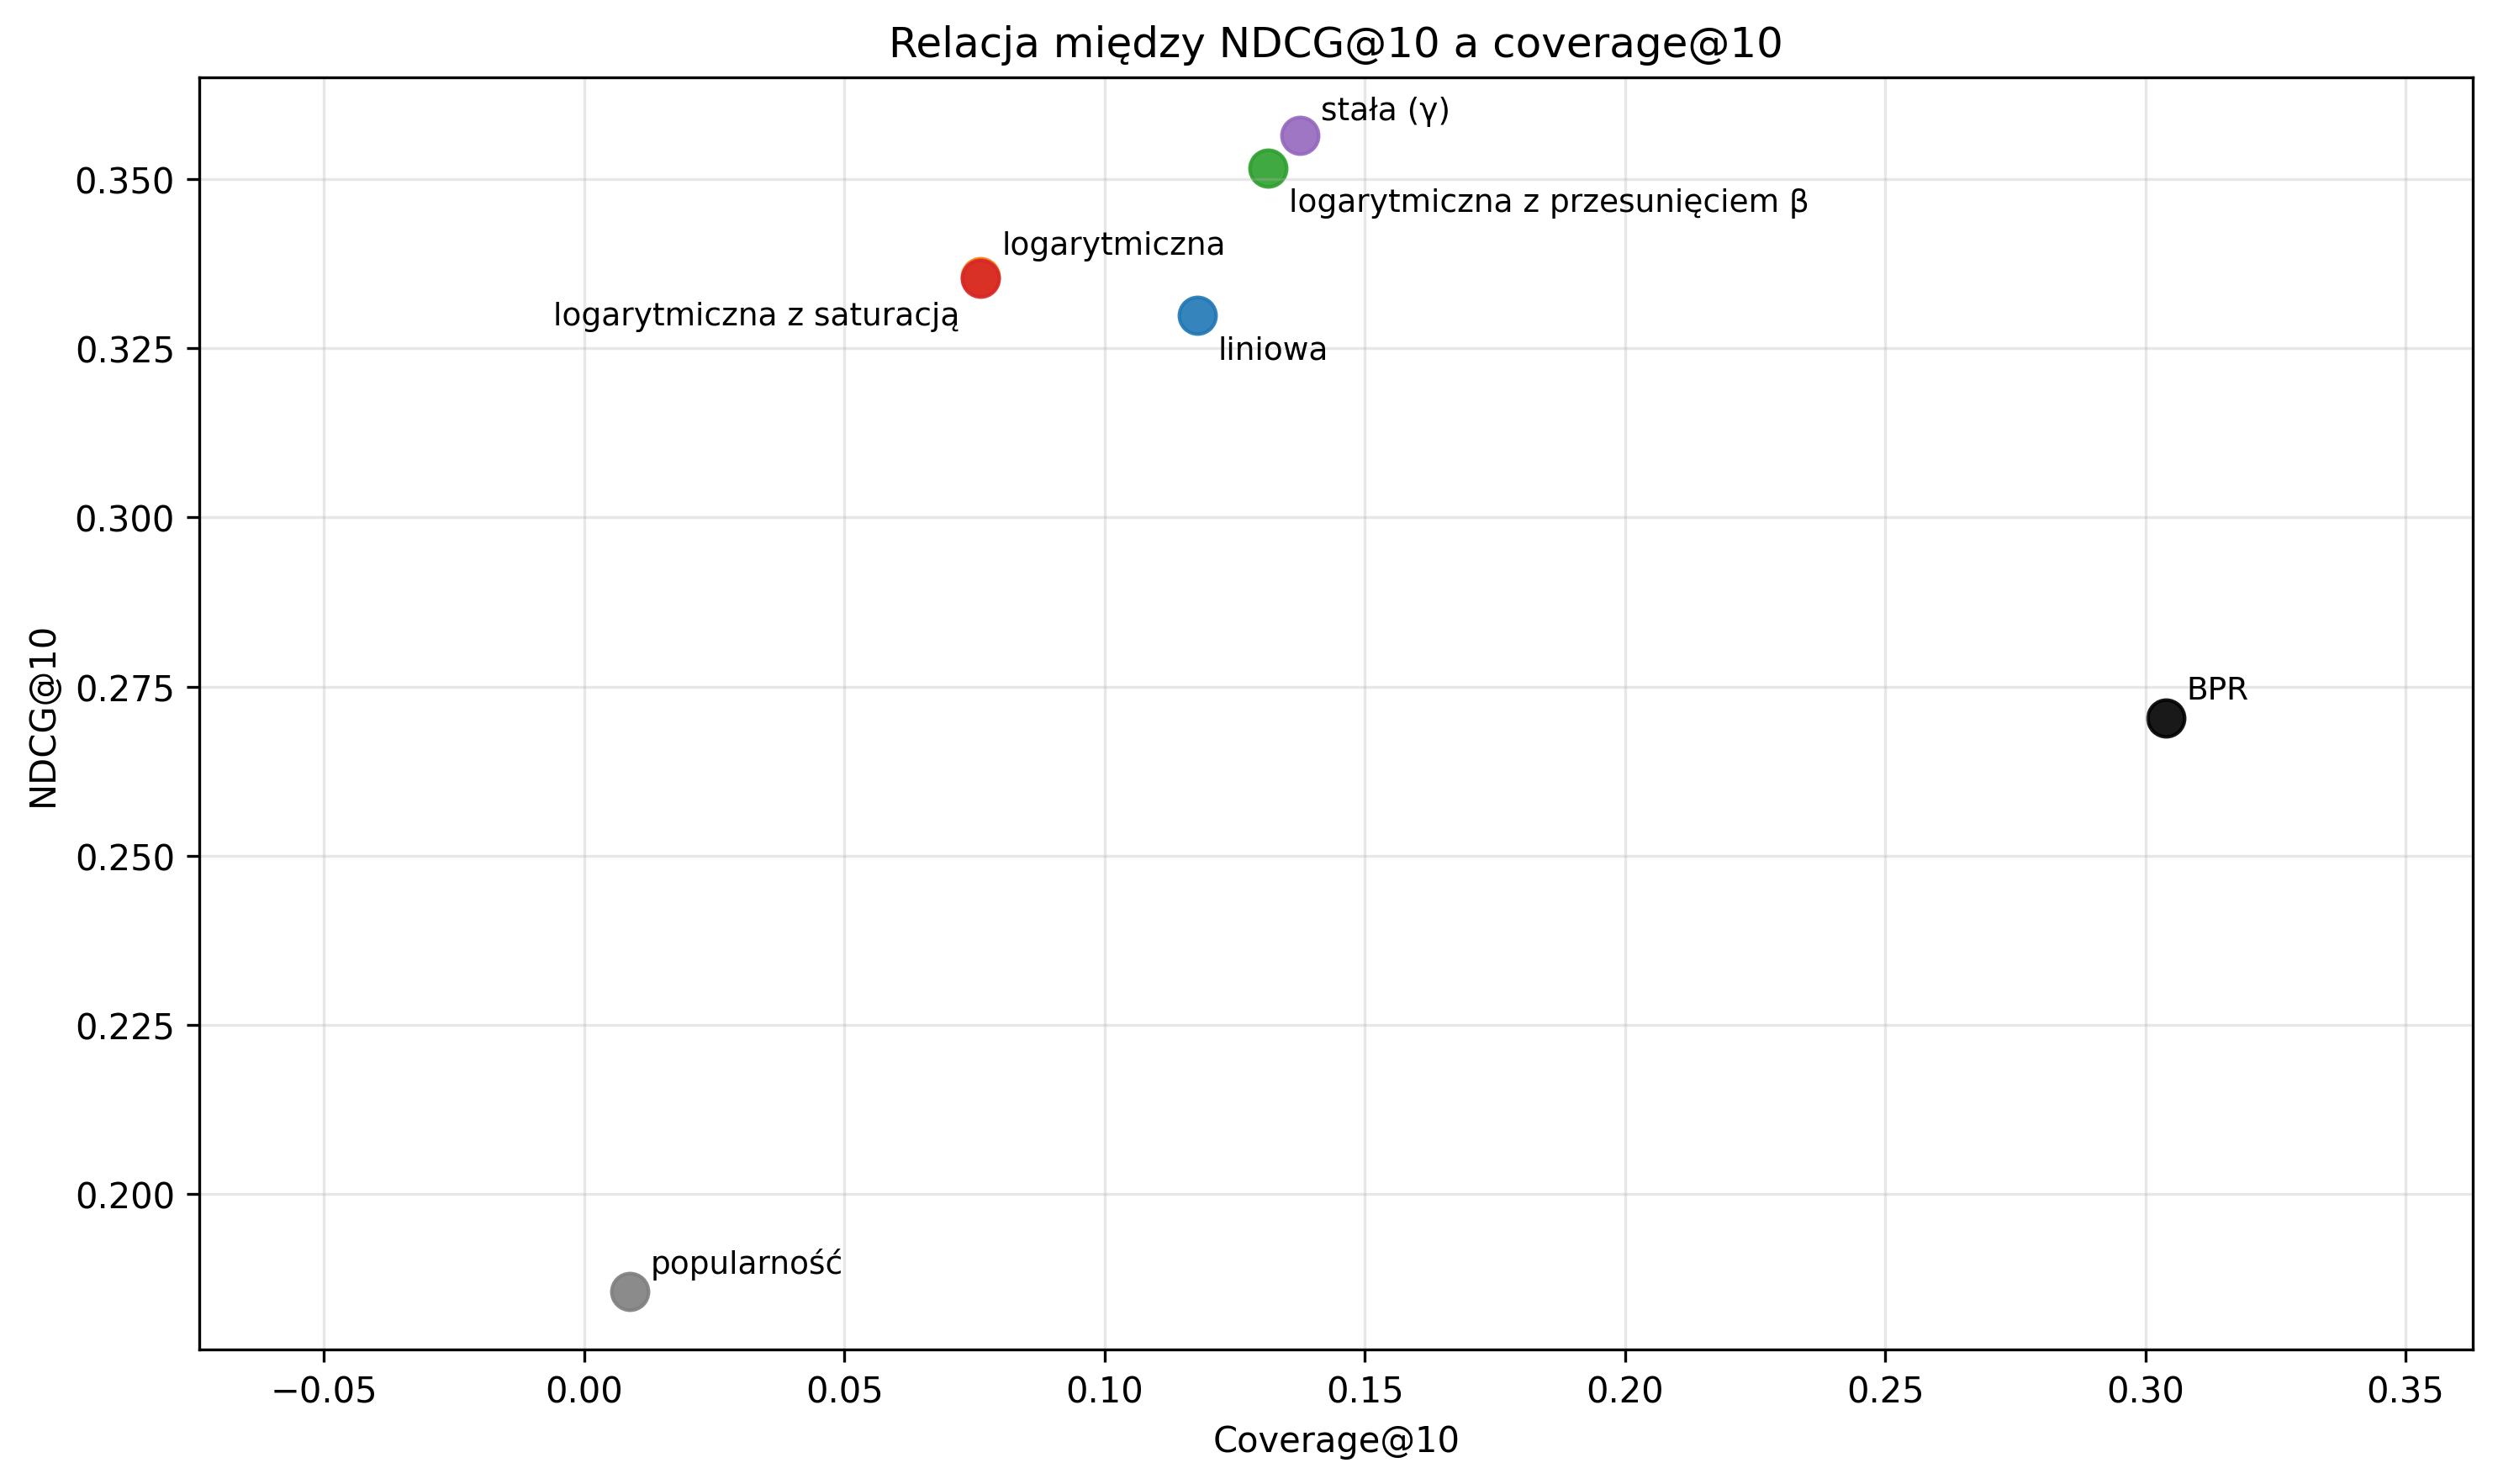
\includegraphics[width=0.9\textwidth]{../results/figures_revised/test_ndcg_vs_coverage_all_models.png}
    \caption{Wartości pokrycia katalogu względem \ndcg{} na zbiorze testowym}
    \label{fig:test_ndcg_vs_coverage_all_models}
\end{figure}

W przypadku metryki pokrycia na wykresie~\ref{fig:test_ndcg_vs_coverage_all_models} widoczna jest znacząca rozbieżność między każdym z badanych typów modeli. Model BPR wykazuje się najwyższym pokryciem (0,3039), będącym ponad dwukrotnie większym niż każdy wariant ALS, jednak osiąga to kosztem niższej wartości \ndcg{}. Rodzina modeli implicit ALS tworzy wyraźne skupienie na wykresie, wewnątrz którego można zaobserwować poprawę wraz ze zwiększeniem bazowej pewności. Najwyższe pokrycie osiąga wariant o stałej funkcji pewności (0,1374), tuż przed wariantem z przesunięciem $\beta$ (0,1313), podczas gdy warianty logarytmiczne pozostają na poziomie około 0{,}076. Oba czołowe warianty wypadają zatem najlepiej pod względem obu przedstawianych metryk, co oznacza, że poprawa jakości rekomendacji nie powstała kosztem faworyzowania wąskiego katalogu obiektów. Niski wynik wariantu popularnościowego pod względem obu metryk jest spójny z oczekiwaniami i wynika z jego niepersonalizowanego charakteru.

Po analizie pokrycia katalogu warto przeanalizować metrykę różnorodności wewnątrzlistowej, opisującą zróżnicowanie pozycji rekomendowanych pojedynczemu użytkownikowi. Miara ta wyznaczana jest na podstawie podobieństwa współwystępowania obiektów w profilach użytkowników w zbiorze treningowym, dzięki czemu pozostaje porównywalna pomiędzy modelami o odmiennych przestrzeniach czynników ukrytych. Model popularnościowy został pominięty w tym porównaniu ze względu na jego niespersonalizowany charakter.

\begin{figure}[htbp]
    \centering
    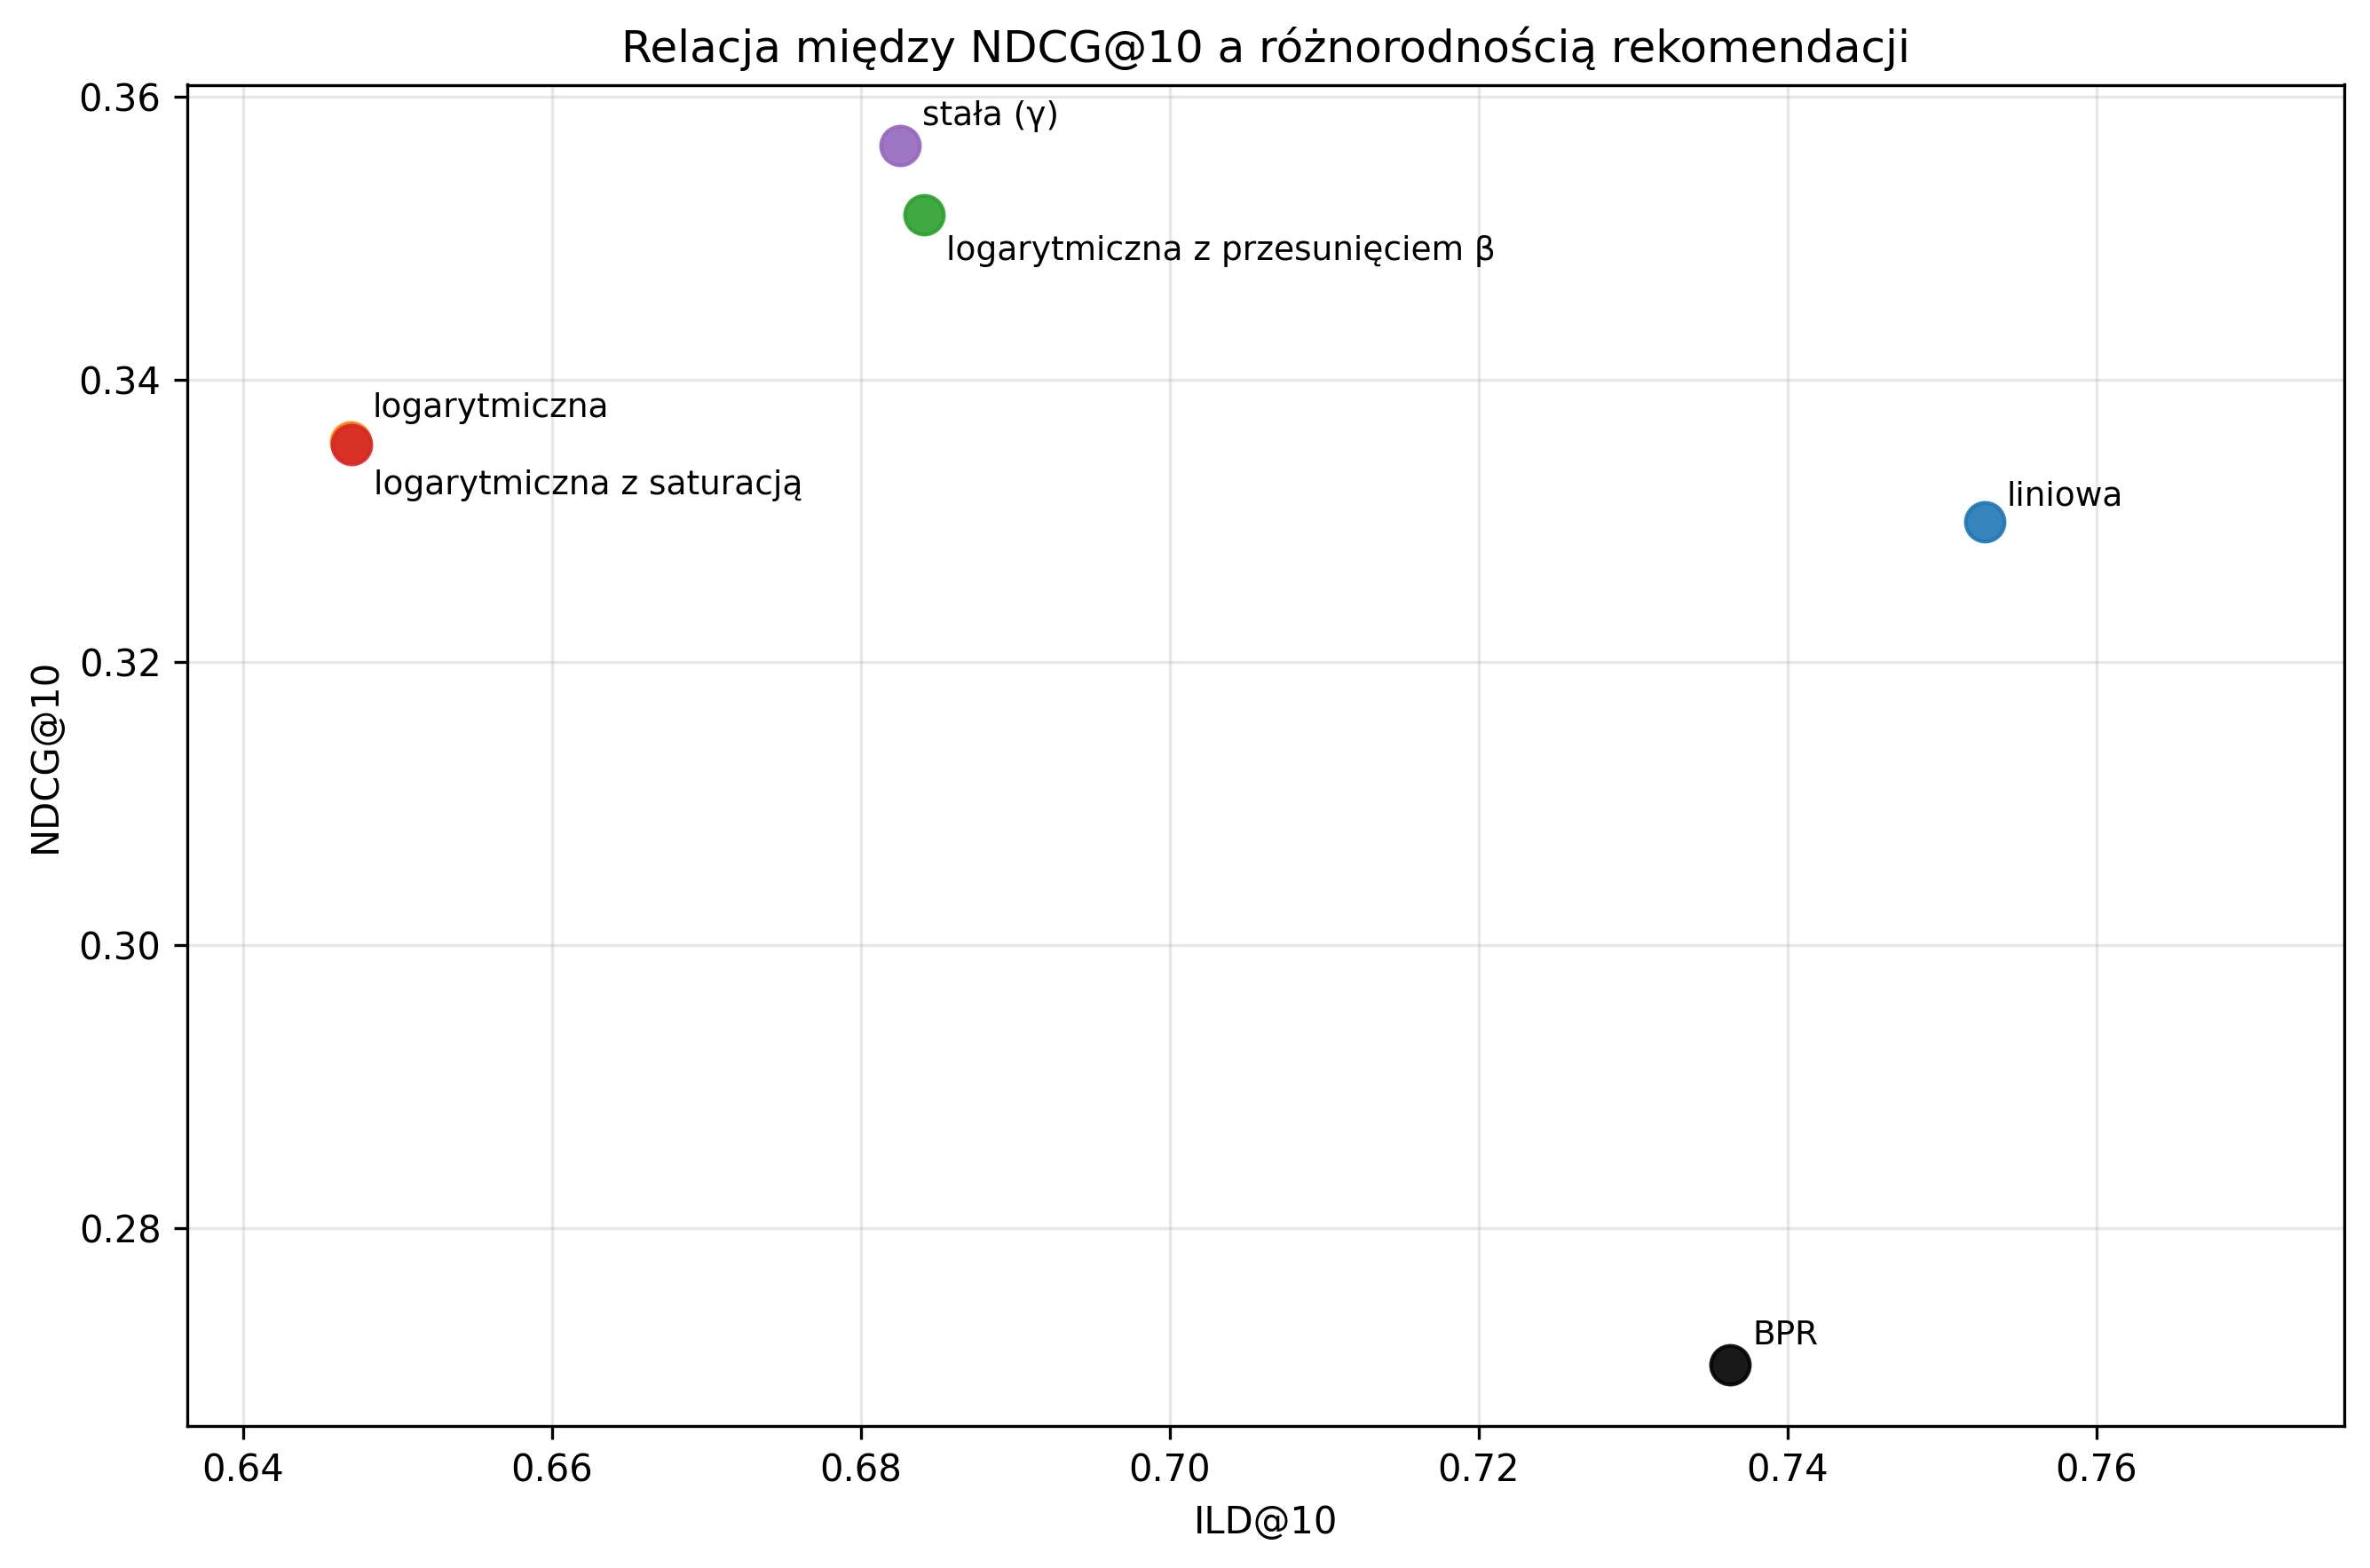
\includegraphics[width=0.9\textwidth]{../results/figures_revised/test_ndcg_vs_ild_cooccurrence.png}
    \caption{Średnie wartości różnorodności wewnątrzlistowej względem \ndcg{} na zbiorze testowym}
    \label{fig:test_ndcg_vs_ild_cooccurrence}
\end{figure}

Na wykresie~\ref{fig:test_ndcg_vs_ild_cooccurrence} zwraca uwagę odrębna pozycja modelu BPR, który przy najniższej wartości \ndcg{} spośród modeli faktoryzacyjnych osiąga wysoką różnorodność (0,7363). W połączeniu z najwyższym pokryciem katalogu wskazuje to, że model ten generuje rekomendacje zarówno silnie zróżnicowane między użytkownikami, jak i wewnątrz jednej listy. Odbywa się to jednak kosztem niższej trafności. Pokazuje to zatem wyraźny kompromis między trafnością a miarami wykraczającymi poza nią.

W obrębie rodziny implicit ALS wartości różnorodności układają się natomiast zgodnie z liczbą czynników ukrytych: warianty logarytmiczne, dysponujące przestrzenią 24-wymiarową, osiągają najniższe wartości (0,6469 oraz 0,6470), warianty stały i z przesunięciem $\beta$ przy 48 czynnikach uzyskują odpowiednio 0,6825 i 0,6841, natomiast wariant liniowy przy 80 czynnikach osiąga wartość najwyższą (0,7528). Warto przy tym zauważyć, że warianty o tej samej wymiarowości uzyskują niemal identyczne wartości, co sugeruje, że wymiar przestrzeni latentnej ma decydujący wpływ na tę metrykę.

Na koniec pozostała do przeanalizowania zależność \ndcg{} od $\Delta\text{GAP}@10$, czyli miary obciążenia rekomendacji popularnością. Wartość zerowa stanowi punkt odniesienia i odpowiada sytuacji, w której popularność rekomendowanych gier jest zbliżona do popularności gier w bibliotece użytkownika zawartych w zbiorze treningowym. Odchylenia w obie strony oznaczają natomiast rekomendowanie pozycji odpowiednio popularniejszych bądź mniej popularnych niż wynikałoby to z profilu użytkownika, przy czym odchylenie w każdą ze stron oznacza rozbieżność z profilem użytkownika. Na wykresie~\ref{fig:test_ndcg_vs_delta_gap_without_popularity} model popularnościowy został ponownie pominięty, aby zachować czytelność pozostałych wyników. Wartość $\Delta\text{GAP}@10$ dla tego modelu wynosi 1,4233, co stanowi maksymalne możliwe obciążenie rekomendacji popularnością w badanym zbiorze.

\begin{figure}[htbp]
    \centering
    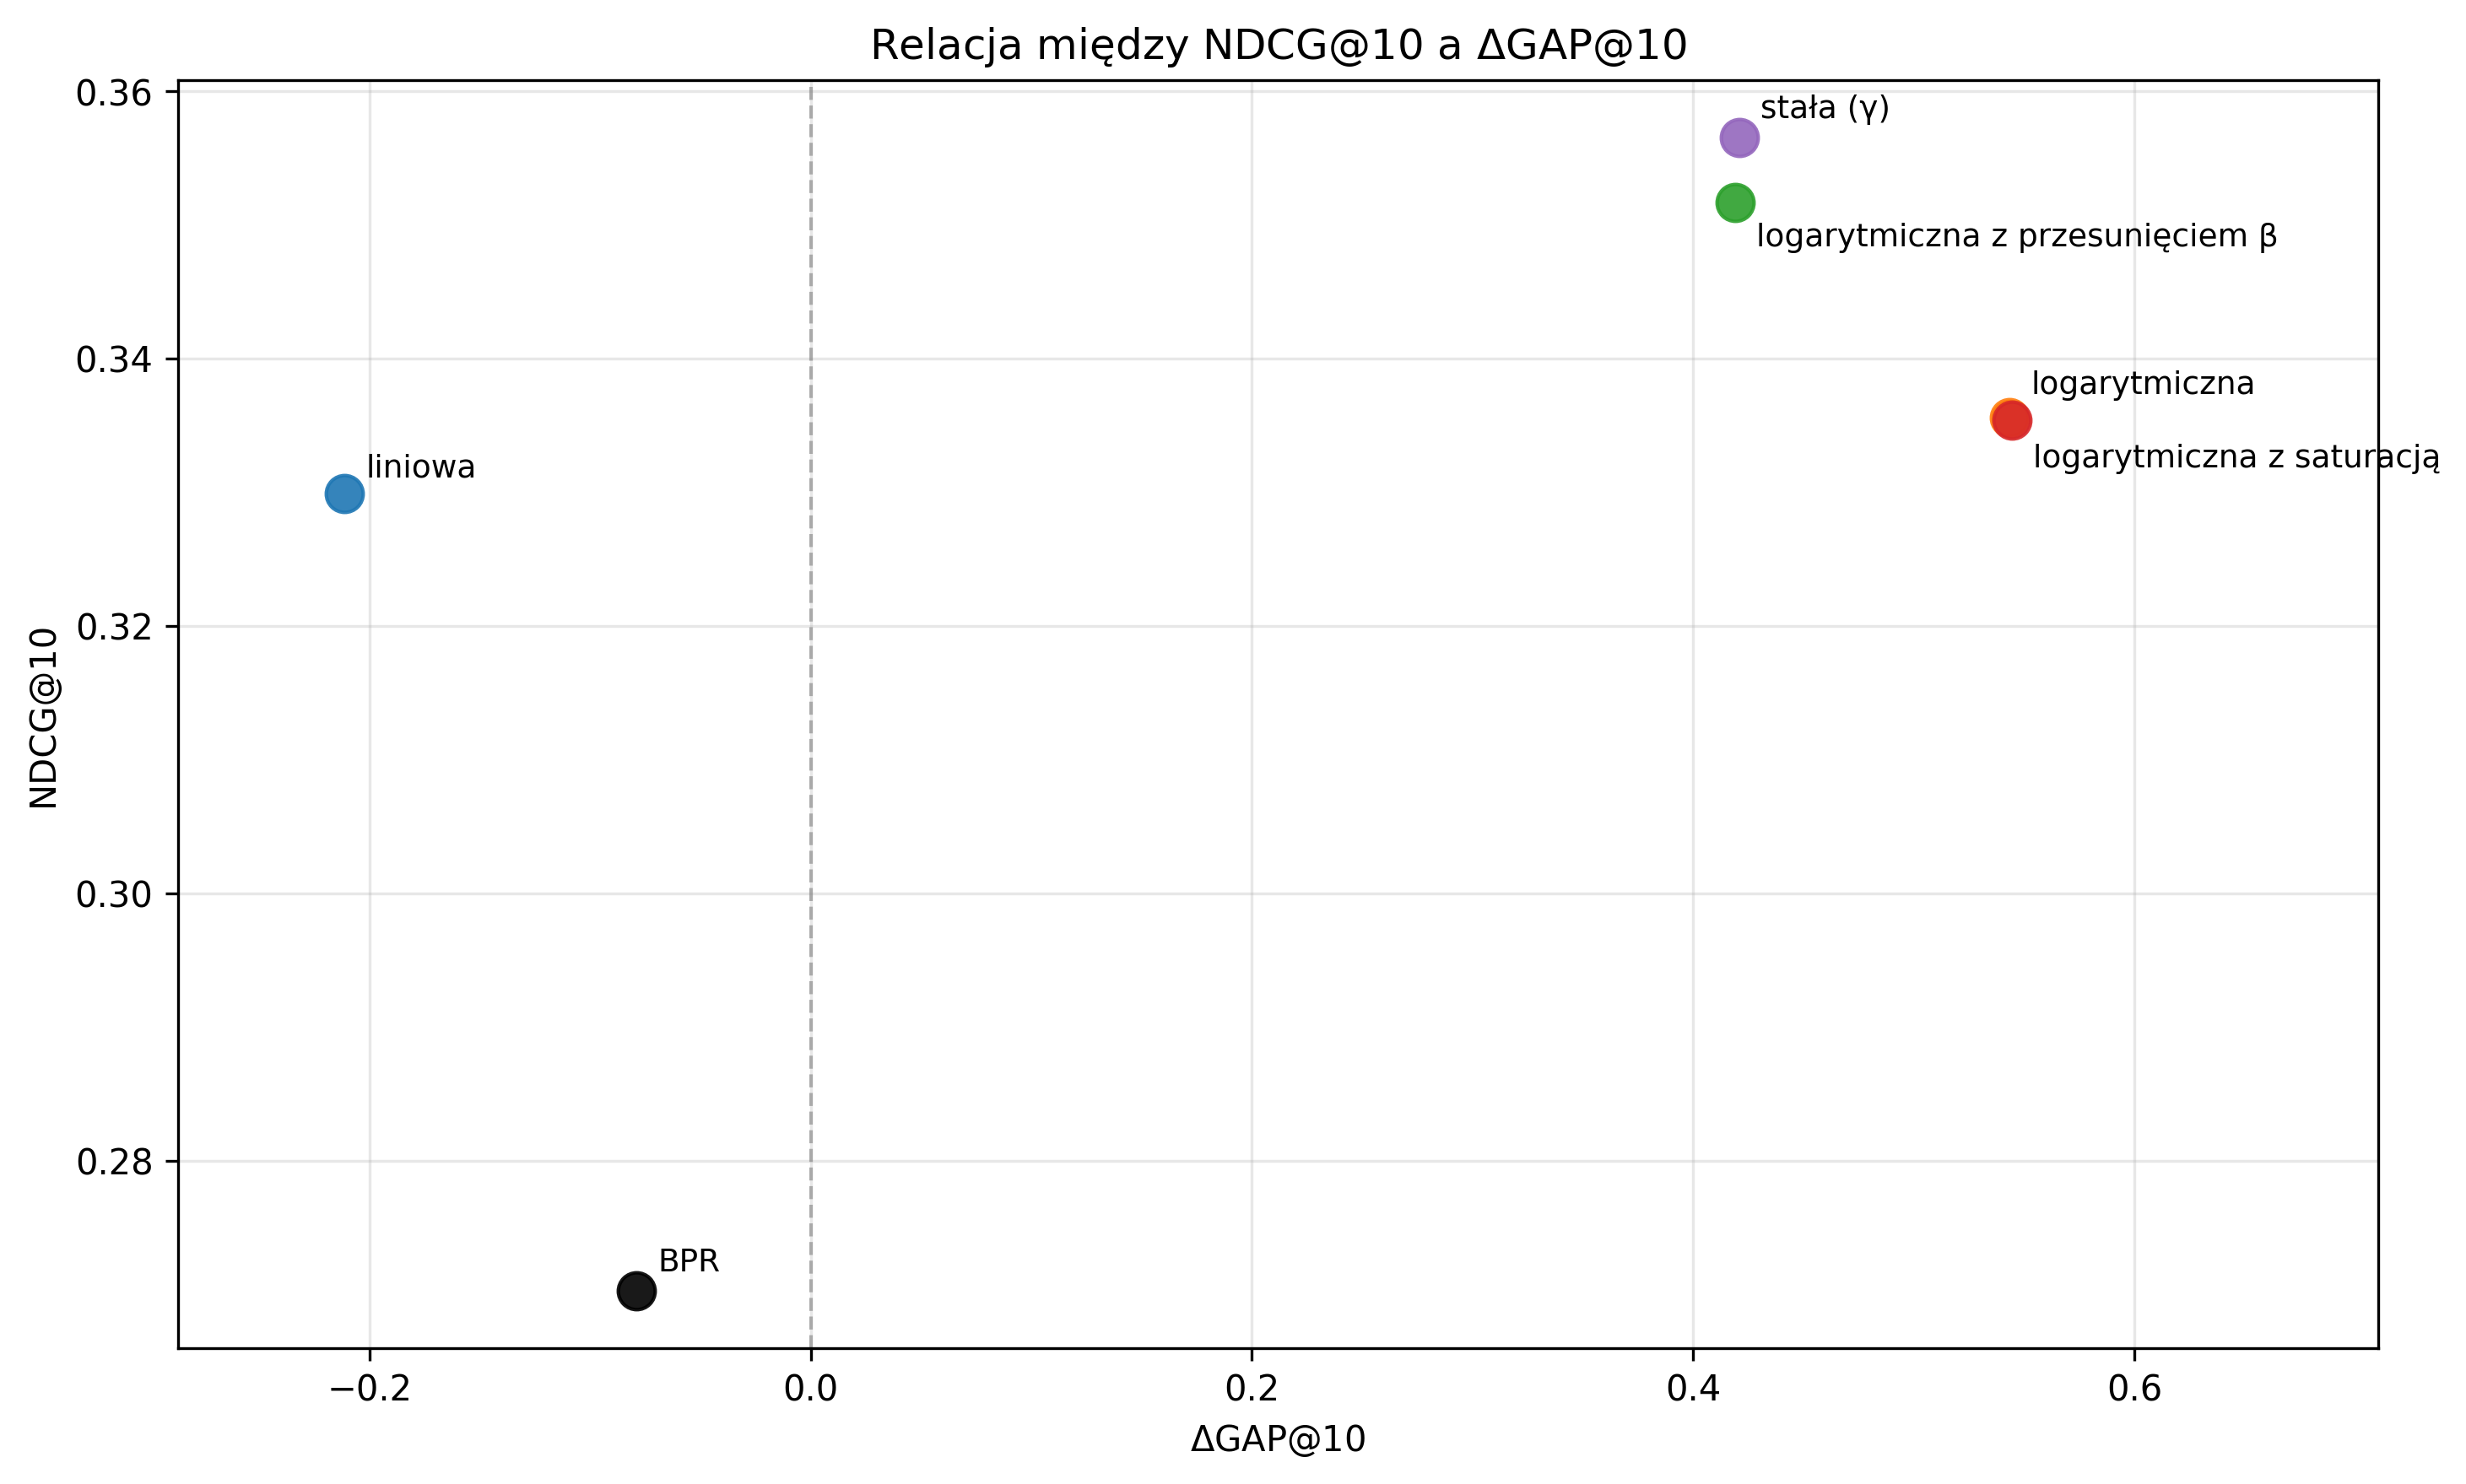
\includegraphics[width=0.9\textwidth]{../results/figures_revised/test_ndcg_vs_delta_gap_without_popularity.png}
    \caption{Średnie wartości $\Delta$GAP względem \ndcg{} na zbiorze testowym}
    \label{fig:test_ndcg_vs_delta_gap_without_popularity}
\end{figure}

Modele BPR oraz implicit ALS z liniową funkcją pewności uzyskały ujemną wartość $\Delta\text{GAP}@10$, co jest nietypowym zachowaniem dla systemów rekomendacyjnych, które mają tendencję do faworyzowania popularnych produktów~\cite{abdollahpouri2019unfairness}. Jednym z~możliwych wyjaśnień jest większa wymiarowość przestrzeni czynników ukrytych obu modeli w~połączeniu ze słabszą regularyzacją. Mniejsza wartość hiperparametrów $\lambda$ oraz $\lambda_\Theta$ dopuszcza wzrost norm wektorów reprezentacji, co umożliwia tworzenie skrajnych dopasowań dla gier o~niskiej popularności. Nie jest to jednak jedyne wyjaśnienie. Ujemna wartość $\Delta\text{GAP}@10$ oznacza odchylenie rekomendacji od profilu użytkownika, które równie dobrze może wynikać ze słabszego dopasowania modelu, a~nie z~trafniejszego rozpoznania preferencji niszowych. Za drugą interpretacją przemawia to, że wariant liniowy osiąga jednocześnie najniższą trafność w~rodzinie implicit ALS. Rozstrzygnięcie między tymi wyjaśnieniami wymagałoby porównania wariantów przy ustalonej liczbie czynników ukrytych, co wykracza poza zakres przeprowadzonego eksperymentu. Wariant liniowy zasługuje przy tym na uwagę, ponieważ łączy ujemną wartość $\Delta\text{GAP}@10$ z największą różnorodnością wewnątrzlistową, jednak traci przy tym na trafności rekomendacji. W przypadku pozostałych modeli ALS ich wartości $\Delta\text{GAP}@10$ są większe od zera, więc rekomendują one gry popularniejsze niż w zbiorze treningowym użytkownika, ale za to cechują się większą trafnością. Na wykresie~\ref{fig:test_ndcg_vs_delta_gap_without_popularity} widać również, że uwzględnienie zwiększonej bazowej wartości pewności nie tylko poprawia trafność rekomendacji, ale również zmniejsza obciążenie popularnością względem wariantów logarytmicznych.

\section{Stabilność wyników}
\label{sec:stabilnosc}

W celu sprawdzenia stabilności wyników obliczono odchylenia standardowe na pięciu uruchomieniach algorytmów implicit ALS i BPR. Wyniki przedstawiono w tabeli~\ref{tab:stabilnosc-zbiorcza}. Metryka ILD@10 została pominięta w analizie stabilności, ponieważ wyznaczono ją dla pojedynczego uruchomienia każdego z modeli.

\begin{table}[htbp]
\centering
\caption{Wyniki na zbiorze testowym wraz z~odchyleniami standardowymi w~pięciu uruchomieniach}
\label{tab:stabilnosc-zbiorcza}
\begin{tabular}{lrrr}
\toprule
Wariant & Precision@10 & Recall@10 & NDCG@10 \\
\midrule
Popularność & $0{,}0965$ & $0{,}1783$ & $0{,}1855$ \\
Liniowa & $0{,}1841\pm0{,}0003$ & $0{,}2642\pm0{,}0005$ & $0{,}3299\pm0{,}0005$ \\
Logarytmiczna & $0{,}1810\pm0{,}0001$ & $0{,}3019\pm0{,}0002$ & $0{,}3356\pm0{,}0003$ \\
Logarytmiczna z saturacją & $0{,}1809\pm0{,}0002$ & $0{,}3019\pm0{,}0003$ & $0{,}3354\pm0{,}0005$ \\
Logarytmiczna z przesunięciem $\beta$ & $0{,}1956\pm0{,}0002$ & $0{,}3338\pm0{,}0003$ & $0{,}3517\pm0{,}0004$ \\
Stała & $0{,}1978\pm0{,}0001$ & $0{,}3370\pm0{,}0002$ & $0{,}3565\pm0{,}0005$ \\
BPR & $0{,}1329\pm0{,}0003$ & $0{,}2614\pm0{,}0005$ & $0{,}2703\pm0{,}0006$ \\
\midrule
Wariant & Coverage@10 & $\Delta$GAP@10 & \\
\midrule
Popularność & $0{,}0087$ & $1{,}4233$ & \\
Liniowa & $0{,}1178\pm0{,}0007$ & $-0{,}2112\pm0{,}0016$ & \\
Logarytmiczna & $0{,}0762\pm0{,}0003$ & $0{,}5433\pm0{,}0008$ & \\
Logarytmiczna z saturacją & $0{,}0761\pm0{,}0002$ & $0{,}5443\pm0{,}0009$ & \\
Logarytmiczna z przesunięciem $\beta$ & $0{,}1313\pm0{,}0009$ & $0{,}4191\pm0{,}0023$ & \\
Stała & $0{,}1374\pm0{,}0004$ & $0{,}4210\pm0{,}0008$ & \\
BPR & $0{,}3039\pm0{,}0012$ & $-0{,}0789\pm0{,}0054$ & \\
\bottomrule
\end{tabular}
\caption*{\footnotesize Wartości dla modeli implicit ALS oraz BPR stanowią średnie z~pięciu uruchomień o~różnym ziarnie inicjalizacji. Model popularnościowy jest deterministyczny, dlatego podano dla niego pojedynczy wynik. Źródło: opracowanie własne.}
\end{table}

Analiza odchyleń standardowych uzyskanych w pięciu losowych inicjalizacjach algorytmów implicit ALS i BPR potwierdza wysoką stabilność wszystkich badanych modeli. W przypadku metryk trafności rekomendacji odchylenia standardowe nie przekraczają $0{,}0006$, co odpowiada mniej niż $0{,}2\%$ wartości średniej. Świadczy to o tym, że przedstawione różnice jakościowe między modelami nie wynikają z losowości inicjalizacji. Z kolei najwyższe odchylenie względne zaobserwowano przy metryce $\Delta$GAP@10 dla modelu BPR, które wynosi $6{,}84\%$ przy wartości średniej równej $-0{,}0789$. Ze względu na znikome różnice wynikające z odchyleń wykresy mające na celu je przedstawić zostały pominięte.

\begin{table}[htbp]
\centering
\caption{Wyniki na zbiorze walidacyjnym wraz z~odchyleniami standardowymi w~pięciu losowych podziałach danych}
\label{tab:stabilnosc-walidacja-zbiorcza}
\begin{tabular}{lrrr}
\toprule
Wariant & Precision@10 & Recall@10 & NDCG@10 \\
\midrule
Popularność & $0{,}0811\pm0{,}0002$ & $0{,}1719\pm0{,}0002$ & $0{,}1615\pm0{,}0004$ \\
Liniowa & $0{,}1360\pm0{,}0006$ & $0{,}2302\pm0{,}0008$ & $0{,}2466\pm0{,}0011$ \\
Logarytmiczna & $0{,}1349\pm0{,}0009$ & $0{,}2589\pm0{,}0019$ & $0{,}2534\pm0{,}0018$ \\
Logarytmiczna z saturacją & $0{,}1350\pm0{,}0008$ & $0{,}2596\pm0{,}0015$ & $0{,}2536\pm0{,}0015$ \\
Logarytmiczna z przesunięciem $\beta$ & $0{,}1479\pm0{,}0005$ & $0{,}2963\pm0{,}0012$ & $0{,}2744\pm0{,}0011$ \\
Stała & $0{,}1502\pm0{,}0003$ & $0{,}3007\pm0{,}0010$ & $0{,}2792\pm0{,}0007$ \\
\midrule
Wariant & Coverage@10 & $\Delta$GAP@10 & \\
\midrule
Popularność & $0{,}0069\pm0{,}0002$ & $1{,}5138\pm0{,}0011$ & \\
Liniowa & $0{,}1025\pm0{,}0003$ & $-0{,}2048\pm0{,}0010$ & \\
Logarytmiczna & $0{,}0636\pm0{,}0006$ & $0{,}4899\pm0{,}0071$ & \\
Logarytmiczna z saturacją & $0{,}0635\pm0{,}0006$ & $0{,}4942\pm0{,}0047$ & \\
Logarytmiczna z przesunięciem $\beta$ & $0{,}1138\pm0{,}0017$ & $0{,}4072\pm0{,}0119$ & \\
Stała & $0{,}1208\pm0{,}0006$ & $0{,}4256\pm0{,}0079$ & \\
\bottomrule
\end{tabular}
\caption*{\footnotesize Analizę przeprowadzono na pięciu losowych podziałach na zbiór treningowy i~walidacyjny przy ustalonym ziarnie inicjalizacji modelu. Źródło: opracowanie własne.}
\end{table}

W związku z zastosowaniem wydzielonego zbioru testowego zamiast procedury walidacji krzyżowej przeprowadzono analizę stabilności względem losowego podziału danych. W tabeli~\ref{tab:stabilnosc-walidacja-zbiorcza} przedstawiono wartości średnie metryk oraz odchylenia standardowe liczone na pięciu losowych podziałach na zbiory treningowe i walidacyjne. Analizę tę ograniczono do modeli implicit ALS oraz modelu popularnościowego. Największą względną wartość odchylenia standardowego odnotowano dla metryki $\Delta$GAP@10 w~wariancie logarytmicznym z~przesunięciem $\beta$, gdzie wynosi ona $2{,}92\%$. Tak niski poziom zmienności wynika najprawdopodobniej ze znacznego rozmiaru wykorzystanego zbioru danych, który uodparnia proces uczenia na~różnice wynikające z~losowego podziału. Ze względu na niewielką skalę odchyleń zrezygnowano z~ich graficznej prezentacji.

\section{Odniesienie wyników do literatury}
\label{sec:porownanie-literatura}

Ograniczona porównywalność i~odtwarzalność wyników stanowi rozpoznany problem w~dziedzinie systemów rekomendacyjnych~\cite{dacrema2019progress}. Z~tego powodu przedstawione rezultaty należy traktować jako zamknięty eksperyment, w~którym wszystkie modele oceniano na tym samym zbiorze, przy identycznej procedurze filtracji, podziału danych oraz ewaluacji. Uzyskane wyniki pozwalają zatem przede wszystkim na porównanie badanych wariantów między sobą w~ramach przyjętej metodologii. Podjęto jednak próbę odniesienia uzyskanych wyników do prac wykorzystujących ten sam zbiór danych.

W~celu weryfikacji poprawności zaimplementowanego procesu trenowania modeli odtworzono wyniki przedstawione w~opracowaniu Bayrama~\cite{bayram2021game}. Stosowana tam metryka, określana przez autora jako Precision@10, odpowiadająca w~praktyce mierze HitRate@10, wyznaczającej odsetek użytkowników, dla których ukryta interakcja znalazła się wśród dziesięciu pierwszych pozycji rankingu. Raportowana wartość wynosi 31,60\%, natomiast w~replikacji uzyskano 29,18\%. Zbieżność obu wyników potwierdza poprawność przyjętej implementacji, a~pozostała różnica wynika przypuszczalnie z~nie w~pełni odtworzonego przygotowania danych, obejmującego między innymi wykorzystanie dodatkowych zbiorów udostępnianych dla platformy Steam. Należy przy tym podkreślić, że w~odtwarzanej pracy zastosowano ewaluację metodą leave-one-out z~próbkowaniem negatywnym, przez co replikacja pełni funkcję kontroli poprawności procesu modelowania, nie zaś punktu odniesienia dla wyników przedstawionych w~niniejszym rozdziale.

Pozostałe badania wykorzystujące dane platformy Steam, do których odnoszono się w~pracy, różnią się od niej w~stopniu uniemożliwiającym zestawienie wartości metryk. Bunga i~in.~\cite{bunga2021implicit} przekształcają czas gry w~ocenę, sprowadzając zadanie do predykcji jawnych ocen, a~ponadto usuwają interakcje z~zerowym czasem gry, użytkowników posiadających mniej niż 30 gier oraz gry występujące u~mniej niż 10 użytkowników. Cheuque i~in.~\cite{cheuque2019steam} koncentrują się natomiast na modelach neuronowych, stosując walidację krzyżową oraz wyraźnie silniejszą filtrację danych. W~obu przypadkach zabiegi te prowadzą do innego zadania ewaluacyjnego niż rozważane w~niniejszej pracy, co znajduje odzwierciedlenie w~różnicach między wartościami raportowanych metryk.
\chapter{Wnioski}

\section{Podsumowanie eksperymentów}

Zakres eksperymentu objął dostrajanie hiperparametrów pięciu wariantów modeli implicit ALS z różnymi wagami pewności (liniowa, logarytmiczna, logarytmiczna z saturacją, logarytmiczna z przesunięciem $\beta$ oraz stała), modelu BPR oraz popularnościowego jako odniesienie. Dobór hiperparametrów pokazał, że w przypadku modeli iALS optymalny hiperparametr $\alpha$ dążył do zera, co w praktyce redukowało sygnał o preferencji płynący z \texttt{playtime\_forever} do wariantu binarnego (użytkownik posiada/nie posiada gry w bibliotece). Jedynym wyjątkiem był model z $c_{ui} = 1 + \alpha \log(1 + r_{ui} + \beta)$, w którym optymalna wartość $\alpha$ nie leżała w otoczeniu zera. Analiza kształtu tego przekształcenia wykazała jednak, że przy $\beta$ równym 108,284 funkcja działa w obszarze o niewielkiej krzywiźnie: dla mediany czasu gry wynoszącej 35 minut wartość $c_{ui}$ wynosi 2,94 wobec 2,83 dla obserwacji bez zarejestrowanego czasu rozgrywki. Wyższa wartość $\alpha$ podnosiła zatem przede wszystkim ogólny poziom pewności, w mniejszym stopniu różnicując obserwacje między sobą.

Obserwacja ta doprowadziła do zbadania granicznego przypadku całej rodziny, czyli wariantu $c_{ui} = 1 + \gamma$, całkowicie pomijającego czas gry. Wariant ten osiągnął najwyższe wyniki metryk rankingowych zarówno na zbiorze walidacyjnym, jak i testowym, poprawiając \ndcg{} o 6,2\% względem wariantu logarytmicznego oraz o 8,1\% względem liniowego. Osiągnął on również największe pokrycie katalogu wśród modeli implicit ALS. Wszystkie różnice okazały się istotne statystycznie (test Wilcoxona z korektą Holma-Bonferroniego, poziom istotności $= 0{,}05$), przy czym analiza wielkości efektu wykazała, że mediana sparowanej różnicy \ndcg{} we wszystkich porównaniach wynosi zero. Obserwowana przewaga ma zatem charakter zagregowany i nie przekłada się na przewidywalną poprawę jakości rekomendacji dla pojedynczego użytkownika.

Badanie pokazało również kompromisy między jakością rankingową a miarami wykraczającymi poza trafność. Model BPR uzyskał ponad dwukrotnie większe pokrycie katalogu niż najlepszy z modeli iALS oraz wysoką różnorodność wewnątrzlistową, ale osiągnął to kosztem znacznie niższej trafności rekomendacji. Natomiast wariant liniowy, mimo najniższej jakości rankingowej w rodzinie iALS, cechuje się największą różnorodnością rekomendacji oraz zdolnością polecania obiektów mniej popularnych niż średnia popularność w zbiorze treningowym danego użytkownika, co jest nietypowym zachowaniem dla modelu opartego na faktoryzacji macierzy.

Przeprowadzona analiza stabilności ze względu na losowe uruchomienia algorytmów oraz podziały danych wykazała wysoką powtarzalność wyników. Odchylenia standardowe metryk trafności nie przekraczały 0,2\% wartości średniej, co oznacza, że obserwowane różnice między wariantami nie wynikają z~losowości procedury.

Powyższe wyniki pozwalają odpowiedzieć na postawione pytania badawcze.

\section{Odpowiedzi na pytania badawcze}

\textbf{PB1. Czy sposób przekształcenia czasu gry na wagi pewności wpływa na jakość rekomendacji modelu implicit ALS?}

Tak, jednak w~kierunku odwrotnym do oczekiwanego. Różnica \ndcg{} między najlepszym a~najgorszym wariantem wynosi 0,0266, co odpowiada poprawie o~8,1\% względem wariantu liniowego. Analiza sparowanych różnic na poziomie użytkownika potwierdza istotność tego efektu: średnia różnica wynosi 0,0266 przy 95-procentowym przedziale ufności $[0{,}0248;\ 0{,}0284]$. Wyższe wyniki osiągnęły jednak te przekształcenia, które w mniejszym stopniu uzależniały wagi pewności od zarejestrowanego czasu rozgrywki. Najwyższą jakość rekomendacji uzyskał wariant całkowicie pomijający tę zmienną, najniższą zaś wariant liniowy, przypisujący wagi proporcjonalne do czasu gry. Należy przy tym podkreślić, że porównywane warianty dostrojono niezależnie, przez co różnią się również liczbą czynników ukrytych oraz siłą regularyzacji. Wniosek dotyczy zatem tego, który wariant po dostrojeniu prowadzi do najlepszych rekomendacji, nie zaś izolowanego wpływu samego przekształcenia sygnału.

\textbf{PB2. Czy różnicowanie wag pewności według czasu gry przewyższa wariant o stałej wadze, niezależnej od intensywności interakcji?}

Nie. Wariant o stałej funkcji pewności uzyskał najwyższą wartość \ndcg{} na zbiorze testowym (0,3565), wyprzedzając wariant z przesunięciem $\beta$ (0,3517) oraz pozostałe przekształcenia. Dwa najlepsze warianty łączy podniesienie pewności obserwacji o zerowym czasie gry, którym pozostałe przekształcenia przypisują wartość równą 1. W badanym zbiorze monotoniczne uwzględnienie zmiennej \texttt{playtime\_forever} nie przyniosło zatem wartości dodanej wykraczającej poza sam wzrost wagi zaobserwowanych par użytkownik--gra.

\textbf{PB3. W jaki sposób wybór funkcji pewności przekłada się na miary wykraczające poza trafność i czy występuje kompromis między trafnością a tymi miarami?}

Odpowiedź różni się w zależności od rozważanej miary. W przypadku pokrycia katalogu kompromis w obrębie rodziny implicit ALS nie występuje: warianty o najwyższej trafności osiągnęły najwyższe pokrycie (0,1374 oraz 0,1313 wobec 0,0762 dla wariantów logarytmicznych). Wartości $\Delta$GAP wskazują natomiast, że wszystkie warianty poza liniowym rekomendują pozycje popularniejsze niż wynikałoby to z profilu użytkownika, przy czym dwa czołowe warianty wykazują umiarkowane obciążenie popularnością (0,4210 oraz 0,4191) wobec wartości powyżej 0,54 dla wariantów logarytmicznych. Warto podkreślić, że ujemna wartość $\Delta$GAP wariantu liniowego ($-0{,}2112$) stanowi odchylenie od punktu neutralnego tak samo jak wartości dodatnie, jedynie w przeciwnym kierunku, i również niekoniecznie jest pożądana. W~przypadku różnorodności wewnątrzlistowej wartości uzyskane w~rodzinie implicit ALS układają się zgodnie z~liczbą czynników ukrytych, dobieraną niezależnie dla każdego wariantu. Nie jest to ograniczenie samej metryki, która wyznaczana jest we~wspólnej dla wszystkich modeli przestrzeni współwystępowania, lecz obserwacja dotycząca zachowania modeli. Model BPR mimo najwyższej liczby czynników osiąga różnorodność niższą niż wariant liniowy. Rozdzielenie wpływu wymiarowości od wpływu samej funkcji pewności wymagałoby jednak eksperymentu przy ustalonej liczbie czynników.

\textbf{PB4. Czy o jakości rekomendacji decyduje w większym stopniu sposób ważenia obserwacji, czy klasa modelu i postać funkcji celu?}

Uzyskane wyniki wskazują na przewagę drugiego z tych czynników. Różnica \ndcg{} między najlepszym wariantem implicit ALS a modelem BPR wynosi 0,0862 i jest ponad trzykrotnie większa niż cały rozstęp wewnątrz rodziny implicit ALS, obejmujący wartości od 0,3299 do 0,3565. Oba porównywane modele traktują przy tym interakcje w sposób nieuwzględniający czasu gry, a~mimo to dzieli je znacznie większa różnica niż którekolwiek dwa warianty funkcji pewności. Także~w~tym przypadku porównanie dotyczy modeli dostrojonych niezależnie, obejmuje zatem łączny efekt zmiany funkcji celu i~towarzyszącego jej doboru pozostałych hiperparametrów. Odpowiedź nie jest jednak jednoznaczna: model BPR uzyskał pokrycie katalogu na poziomie 0,3039, ponad dwukrotnie przewyższające najlepszy wariant implicit ALS. Wybór klasy modelu determinuje zatem nie tylko poziom jakości rekomendacji, lecz także kompromisy między poszczególnymi jej aspektami.

\section{Najważniejsze wnioski praktyczne i metodologiczne}

\subsection{Wnioski praktyczne}

Proste przekształcenia funkcji pewności w przypadku danych o dużym zakresie są podatne na dwa przeciwstawne błędy. Liniowa funkcja jest wrażliwa na wartości odstające, natomiast przekształcenia logarytmiczne są wrażliwe na szum wśród małych wartości. W obu przypadkach proces optymalizacji hiperparametrów reagował w ten sam sposób, dobierając wartości $\alpha$ na tyle małe, że przekształcenie sprowadzało się w praktyce do postaci niemal stałej.

W badanym zbiorze informacja o~samym posiadaniu gry wystarczyła, by uzyskać rekomendacje nie gorsze niż przy uwzględnieniu czasu gry, a~dodatkowy sygnał płynący z~długości interakcji nie przełożył się na ich jakość. Kluczowe znaczenie ma natomiast poziom wagi przypisanej zaobserwowanym interakcjom, stanowiący pełnoprawny hiperparametr wymagający strojenia niezależnie od postaci przekształcenia.

Wybór modelu powinien wynikać z~przyjętych celów systemu rekomendacyjnego. Jeżeli priorytetem jest trafność rekomendacji, wariant iALS o stałej funkcji pewności jest najlepszym wyborem, oferując jednocześnie najwyższe pokrycie katalogu w swojej rodzinie. W przypadku gdy cenniejsze jest szerokie pokrycie katalogu oraz zróżnicowanie rekomendacji między użytkownikami, warto rozważyć model BPR, akceptując wyraźnie niższą trafność.

Redukcja regularyzacji i zwiększenie wymiaru przestrzeni cech ukrytych $f$ mogą zmniejszać obciążenie popularnością $\Delta$GAP, co zaobserwowano w przypadku wariantu liniowego ALS oraz modelu BPR, osiągających ujemne wartości tej metryki. Należy jednak zachować ostrożność przy interpretacji tego efektu: wariant liniowy uzyskał jednocześnie najwyższą różnorodność rekomendacji i najniższą trafność w swojej rodzinie, co sugeruje, że obserwowane wartości mogą wynikać ze słabszego dopasowania modelu, a nie z lepszego rozpoznania niszowych preferencji.

\subsection{Wnioski metodologiczne}

Dokładna analiza wrażliwości hiperparametrów pozwoliła zinterpretować nie tylko to, co osiąga dany model, ale również dlaczego otrzymywane są takie wyniki. Dodatkowo wizualizacja funkcji pewności wraz z zakresem przyjmowanych przez nie wartości umożliwiła wykrycie, że przekształcenia formalnie różnicujące sygnał działają w praktyce w wąskim przedziale, czego sama wartość metryki nie ujawnia.

Szczególnie istotne okazało się uwzględnienie wariantu granicznego, pomijającego badaną zmienną w całości. Bez niego obserwowana poprawa kolejnych przekształceń zostałaby przypisana lepszemu odwzorowaniu siły preferencji, podczas gdy wyniki wskazują, że była związana przede wszystkim z podniesieniem ogólnego poziomu pewności.

Nie mniej ważna jest konieczność wielowymiarowej oceny modeli rekomendacyjnych, uwzględniającej zarówno metryki trafności, jak i metryki wykraczające poza nią. Poleganie wyłącznie na \ndcg{} daje niepełny obraz jakości systemu rekomendacyjnego. Istotny jest przy tym dobór samych metryk: pierwotnie rozważana miara różnorodności, oparta na odległościach w przestrzeni czynników ukrytych, okazała się nieporównywalna między modelami o odmiennej wymiarowości, co wymusiło jej zastąpienie miarą opartą na współwystępowaniu obiektów we wspólnej dla wszystkich modeli przestrzeni.

W analizie należy również uwzględnić testy stabilności modelu ze względu na losowość podziału danych oraz inicjalizacji algorytmów, jak i testy istotności statystycznej różnic. Przy dużej liczbie użytkowników sama istotność statystyczna nie jest jednak wystarczającą podstawą do wnioskowania i wymaga uzupełnienia miarami wielkości efektu wraz z przedziałami ufności.

\section{Kierunki dalszych badań}

Kierunkiem wynikającym bezpośrednio z uzyskanych wyników, stanowiącym autorską propozycję, jest zbadanie niemonotonicznych funkcji pewności. Wszystkie przekształcenia rozważane w niniejszej pracy były monotonicznie rosnące, przyjmując założenie, że dłuższy czas gry oznacza silniejszą preferencję. Założenie to może jednak nie odpowiadać rzeczywistym zachowaniom użytkowników. W szczególności krótka interakcja, obejmująca kilkanaście czy kilkadziesiąt minut rozgrywki, może świadczyć nie o słabej preferencji, lecz o uruchomieniu gry i szybkiej rezygnacji z niej, stanowiąc tym samym sygnał negatywny. W takim ujęciu obserwacje o zerowym czasie gry, odpowiadające samemu posiadaniu tytułu w bibliotece, niosłyby silniejszy sygnał preferencji niż obserwacje o bardzo krótkim czasie rozgrywki. Funkcja pewności odzwierciedlająca ten wzorzec musiałaby przypisywać obniżone wagi w wąskim przedziale niskich wartości \texttt{playtime\_forever}, a rosnące dopiero powyżej pewnego progu. Zbadanie takiego wariantu pozwoliłoby zweryfikować, czy brak wartości dodanej z czasu gry zaobserwowany w niniejszej pracy wynika z samej zmiennej, czy z założenia o monotonicznym charakterze jej związku z preferencją.

Rozwinięciem tej propozycji jest konstrukcja funkcji pewności, w~której poziom bazowy oraz człon zależny od czasu gry sterowane byłyby niezależnymi parametrami. W~wariancie z~przesunięciem $\beta$ obie składowe pozostają sprzężone: ten sam parametr wyznacza wartość przypisaną obserwacjom zerowym i~stopień kompresji różnic między pozostałymi. Nie pozwala to rozstrzygnąć, czy człon zależny od czasu gry obniżał jakość rekomendacji, czy jedynie nie wnosił poprawy przy jednoczesnym ustawieniu poziomu bazowego poniżej wartości optymalnej. Rozdzielenie tych parametrów, w~połączeniu z~dopuszczeniem niemonotonicznej postaci członu zależnego od czasu gry, umożliwiłoby zbadanie obu mechanizmów osobno.

Wyniki metryk $\Delta$GAP i pokrycia pokazały, że modele ALS (poza wariantem liniowym) mają tendencję do faworyzowania popularnych pozycji. Potencjalnym rozwiązaniem byłoby wprowadzenie do funkcji $c_{ui}$ lub do funkcji straty czynnika odwrotnie proporcjonalnego do popularności danego obiektu. Metody tego typu są opisywane w literaturze jako debiasing z wykorzystaniem odwrotnego ważenia prawdopodobieństwa ekspozycji (ang. \textit{inverse propensity scoring}, IPS), gdzie waga interakcji jest skalowana odwrotnie do prawdopodobieństwa, że dany obiekt zostałby zaobserwowany przez użytkownika niezależnie od jego rzeczywistych preferencji~\cite{schnabel2016recommendations}. W praktyce prawdopodobieństwo to jest zwykle estymowane na podstawie popularności obiektu, ponieważ użytkownicy z większym prawdopodobieństwem wchodzą w interakcję z obiektami popularnymi niezależnie od indywidualnych preferencji. Taka transformacja mogłaby podnosić wagę interakcji z niszowymi grami, kompensując mechanizm, przez który obecne funkcje marginalizują rzadkie obserwacje.

Poza modyfikacją samej funkcji pewności, alternatywnym kierunkiem jest wykorzystanie dopełniających się właściwości testowanych rodzin modeli poprzez ich połączenie w model hybrydowy. Przykładowo model BPR generowałby szeroki wachlarz kandydatów ze względu na większe pokrycie zbioru, a następnie przeprowadzany byłby ponowny ranking przez model iALS cechujący się większą trafnością.

Uzupełnieniem kierunków wynikających z~głównych wniosków pracy są badania wskazane jako ograniczenia przyjętej metodologii:

\begin{itemize}
    \item segmentację użytkowników według liczby posiadanych interakcji,
    umożliwiającą zweryfikowanie hipotezy o~wyższej precyzji wariantu liniowego
    dla użytkowników o~większej aktywności;

    \item uwzględnienie różnic w~zaangażowaniu wynikających ze specyfiki gatunków. Godzina spędzona w~krótkiej produkcji niezależnej oznacza inny poziom zainteresowania niż godzina w~grze wieloosobowej o~dużej regrywalności, tymczasem rozważane funkcje pewności przypisują obu tym obserwacjom identyczną wagę;

    \item eksperyment przy ustalonej, jednakowej liczbie czynników ukrytych dla
    wszystkich wariantów, pozwalający rozdzielić wpływ wymiarowości od wpływu
    samej funkcji pewności na metryki różnorodności i~pokrycia. Przeszukanie przestrzeni obejmującej łącznie parametry funkcji pewności, siłę regularyzacji oraz liczbę czynników ukrytych umożliwiłoby ponadto ustalenie, w~jakim stopniu wielkości te oddziałują na siebie wzajemnie;

    \item powtórzenie eksperymentu na danych ograniczonych do interakcji z niezerowym czasem rozgrywki, stanowiących około dwóch trzecich zbioru, oraz zbadanie wrażliwości wyników na przyjęte progi filtracji. Pozwoliłoby to ustalić, czy brak wartości dodanej wynika z~właściwości samej zmiennej, czy z~decyzji podjętych na etapie przygotowania danych;

    \item porównanie dostrojonego wariantu implicit ALS z~modelami neuronowymi,
    nawiązujące do wyników przedstawionych w~pracy~\cite{rendle2021revisiting};

    \item walidację uzyskanych wyników na innych zbiorach danych i~domenach,
    pozwalającą ustalić, czy zaobserwowany brak przewagi wariantów
    różnicujących jest właściwością uniwersalną, czy wynika z~charakterystyki
    rozkładu długości interakcji w~badanym zbiorze.
\end{itemize}

% ------------------- Bibliografia ---------------------
\printbibliography[heading=bibintoc,title={Bibliografia}]

% ------------------- Wykazy końcowe ---------------------
\chapter*{Wykaz symboli i skrótów}
\addcontentsline{toc}{chapter}{Wykaz symboli i skrótów}

\section*{Skróty}

\begin{longtable}{@{}p{0.18\textwidth}p{0.78\textwidth}@{}}
ALS & naprzemienna metoda najmniejszych kwadratów (\textit{alternating least squares}) \\
iALS & ALS dla niejawnej informacji zwrotnej (\textit{implicit ALS}) \\
BPR & spersonalizowany ranking bayesowski (\textit{Bayesian Personalized Ranking}) \\
SVD & rozkład według wartości osobliwych (\textit{singular value decomposition}) \\
TPE & estymator drzewiasty Parzena (\textit{tree-structured Parzen estimator}) \\
RMSE & pierwiastek błędu średniokwadratowego (\textit{root mean squared error}) \\
MAE & średni błąd bezwzględny (\textit{mean absolute error}) \\
DCG & skumulowany zysk z~dyskontowaniem (\textit{discounted cumulative gain}) \\
IDCG & idealny DCG (\textit{ideal DCG}) \\
NDCG & znormalizowany DCG (\textit{normalized DCG}) \\
ILD & różnorodność wewnątrzlistowa (\textit{intra-list diversity}) \\
GAP & średnia popularność grupy (\textit{group average popularity}) \\
$\Delta$GAP & względna różnica średniej popularności rekomendacji i~profilu użytkownika \\
IPS & odwrotne ważenie prawdopodobieństwem ekspozycji (\textit{inverse propensity scoring})
\end{longtable}

\section*{Symbole}

\begin{longtable}{@{}p{0.18\textwidth}p{0.78\textwidth}@{}}
\multicolumn{2}{@{}l}{\textit{Zbiory i~indeksy}} \\[2pt]
$\mathcal{U}$ & zbiór użytkowników, $|\mathcal{U}| = m$ \\
$\mathcal{I}$ & zbiór obiektów (gier), $|\mathcal{I}| = n$ \\
$u$ & indeks użytkownika, $u \in \mathcal{U}$ \\
$i$, $j$ & indeksy obiektów, $i, j \in \mathcal{I}$ \\
$k$, $l$ & indeksy pozycji na liście rekomendacyjnej \\
$\mathcal{I}_u$ & zbiór obiektów, z~którymi użytkownik $u$ wszedł w~interakcję \\
$\mathcal{I}_u^{+}$ & zbiór obiektów pozytywnych użytkownika $u$ w~modelu BPR \\
$\mathcal{I}_u^{\text{train}}$, $\mathcal{I}_u^{\text{test}}$ & interakcje użytkownika $u$ w~zbiorze treningowym i~testowym \\
$\mathcal{K}$ & zbiór zaobserwowanych par $(u,i)$ \\
$\mathcal{K}_{\text{conf}}$ & zbiór par, dla których $c_{ui} \neq 1$ \\
$D_S$ & zbiór trójek treningowych $(u,i,j)$ w~modelu BPR \\
$>_u$ & ukryta relacja preferencji użytkownika $u$ \\[6pt]

\multicolumn{2}{@{}l}{\textit{Dane i~preferencje}} \\[2pt]
$\mathbf{R}$ & macierz obserwacji, $\mathbf{R} \in \mathbb{R}^{m \times n}$ \\
$r_{ui}$ & zarejestrowana intensywność interakcji użytkownika $u$ z~obiektem $i$ (czas gry) \\
$\mathbf{P}$ & binarna macierz preferencji, $\mathbf{P} \in \{0,1\}^{m \times n}$ \\
$p_{ui}$ & element macierzy preferencji; $p_{ui} = 1$, gdy obiekt $i$ znajduje się w~bibliotece użytkownika $u$ \\
$\mathbf{p}^u$, $\mathbf{p}^i$ & wektory preferencji użytkownika $u$ oraz obiektu $i$ \\
$\mathbf{p}_i$ & kolumna macierzy $\mathbf{P}$ odpowiadająca obiektowi $i$ \\[6pt]

\multicolumn{2}{@{}l}{\textit{Model i~parametry}} \\[2pt]
$\mathbf{X}$, $\mathbf{Y}$ & macierze czynników ukrytych użytkowników i~obiektów \\
$\mathbf{x}_u$, $\mathbf{y}_i$ & wektory czynników ukrytych, $\mathbf{x}_u, \mathbf{y}_i \in \mathbb{R}^f$ \\
$f$ & wymiar przestrzeni czynników ukrytych \\
$\Theta$ & wektor wszystkich parametrów modelu BPR \\
$\mu$, $b_u$, $b_i$ & wyraz wolny oraz odchylenia użytkownika i~obiektu w~modelu Funk SVD \\
$\hat{r}_{ui}$ & przewidywana wartość oceny \\
$\hat{s}_{ui}$ & wynik dopasowania obiektu $i$ do użytkownika $u$ w~modelu BPR \\
$\hat{s}_{uij}$ & różnica wyników dopasowania, $\hat{s}_{uij} = \hat{s}_{ui} - \hat{s}_{uj}$ \\
$\mathbf{C}^u$, $\mathbf{C}^i$ & diagonalne macierze pewności użytkownika $u$ oraz obiektu $i$ \\
$c_{ui}$ & waga pewności przypisana parze użytkownik--obiekt \\
$\mathbf{I}_f$, $\mathbf{I}_n$ & macierze jednostkowe wymiaru $f$ oraz $n$ \\[6pt]

\multicolumn{2}{@{}l}{\textit{Hiperparametry}} \\[2pt]
$\alpha$ & parametr skalujący wagę pewności \\
$\beta$ & parametr przesunięcia w~przekształceniu logarytmicznym \\
$\gamma$ & stała wartość wzrostu wagi pewności w~wariancie niezależnym od czasu gry \\
$\lambda$ & współczynnik regularyzacji w~modelach Funk SVD oraz iALS \\
$\lambda_\Theta$ & współczynnik regularyzacji w~modelu BPR \\
$\eta$ & współczynnik uczenia w~algorytmie LearnBPR \\[6pt]

\multicolumn{2}{@{}l}{\textit{Ewaluacja}} \\[2pt]
$N$ & długość listy rekomendacyjnej \\
$\mathcal{R}_u^N$ & zbiór obiektów rekomendowanych użytkownikowi $u$ \\
$\text{Hits}_u@N$ & liczba trafnych rekomendacji dla użytkownika $u$ \\
$\text{pop}(i)$ & popularność obiektu $i$ \\
$d_{\cos}(i,j)$ & odległość cosinusowa między obiektami $i$ oraz $j$ \\[6pt]

\multicolumn{2}{@{}l}{\textit{Funkcje}} \\[2pt]
$\sigma(\cdot)$ & funkcja sigmoidalna \\
$\mathbf{1}(\cdot)$ & funkcja wskaźnikowa \\
$\mathcal{L}$ & funkcja celu \\
$\operatorname{vec}(\cdot)$ & przekształcenie macierzy do postaci wektora
\end{longtable}

\addcontentsline{toc}{chapter}{Spis rysunków}
\listoffigures
\thispagestyle{plain}

\addcontentsline{toc}{chapter}{Spis tabel}
\listoftables
\thispagestyle{plain}

%\chapter*{Załączniki}
%\addcontentsline{toc}{chapter}{Załączniki}
%\appendix
%\chapter{Dodatkowe tabele wyników}

% TODO: opcjonalne dodatkowe tabele wyników.

\chapter{Dodatkowe wykresy}

% TODO: opcjonalne dodatkowe wykresy.

\chapter{Struktura plików projektu i reprodukowalność}

% TODO: opis struktury plików projektu i informacji potrzebnych do reprodukcji.


\end{document}
